\documentclass{report}
\usepackage[utf8]{inputenc}
\usepackage[english]{babel}
\usepackage[]{graphicx}
\graphicspath{ {Figures/} }
\usepackage{multirow}
\usepackage{enumitem}
\usepackage{tabularx}
\usepackage{booktabs}
\usepackage{ltablex}
\usepackage{amsmath}
\usepackage[parfill]{parskip}
% Set page margins
\usepackage[top=100pt,bottom=100pt,left=68pt,right=66pt]{geometry}
% Changes the style of chapter headings
\usepackage{titlesec}
\titleformat{\chapter}
   {\normalfont\LARGE\bfseries}{\thechapter.}{1em}{}
% Change distance between chapter header and text
\titlespacing{\chapter}{0pt}{50pt}{2\baselineskip}
\newcommand{\tabincell}[2]{\begin{tabular}{@{}#1@{}}#2\end{tabular}} 
\usepackage[usestackEOL]{stackengine}

\pagenumbering{roman}

\begin{document}
% Title
\begin{titlepage}
	\clearpage\thispagestyle{empty}
	\centering
	\vspace{1cm}

	% Titles
	% Information about the University
	{\normalsize The University of Melbourne \\ 
		School of Computing and Information Systems \\
		SWEN90016 Software Processes and Management\\
		Semester 1 – 2020 \par}
	\vspace{3cm}

	{\Huge \textbf{JJFresh -- Project Management Plan}} \\
  \vspace{0.5cm}
	{\normalsize Version 1.1 \par}
	%{\large \textbf{xxxxx} \par}
	\vspace{2.5cm}
	{\normalsize Zhaofeng Qiu 1101584\\ % \\ specifies a new line
	             Chongjing Zhang 1055520\\
	             Pin Wang 1056745 \\
	             Yicun Tian 1088217 \\
	             Hongkang Li 977063\par}
	\vspace{3cm}
    
  \centering 
\includegraphics[scale=0.12]{logo.pdf}
  
  \vspace{0.5cm}
		
	% Set the date
	{\normalsize \today \par}
	\pagebreak
\end{titlepage}

\chapter*{Executive Summary}
  The project's goal is to provide Jess and James with an online store for selling their fruit and vegetable, which is expected to increase their revenue. Jess and James are the Bussiness Owners of the project. The teaching team of SWEN90016 would take the role of Subject Matter Expert to help the student team. The customers of JJFresh would be our main external stakeholders.

  All the in-scope and out-scope requirements of the project have been defined and confirmed by Jess and James. Base on the consideration of flexibility and the speed of website delivery, Scrum is chosen as our software development cycle model.

  The business value of this project is to meet the need of the people who want to buy fruit and vegetables from JJFresh but cannot go during the business hours of the physical store. The increase in orders would also increase the revenue of the store. The teaching team can improve their experience in teaching while the student team can gain software development experience from the project. Moreover, fruit and vegetable suppliers can also get more orders from Jess and James. The risks of the project have been analyzed, and possible solutions for them are also provided in this report. 

  The technology we choose to implement the online store is \textit{Wix}. The student team is a virtual team and the basic communication tools are \textit{Zoom} and \textit{Slack}. Our communication plan is detailed.

  The project development will take at most 5 weeks, from April 27 to May 8, 2020. We plan to finish the project within 4 weeks. The development of the project will not consume any funds. But if Jess and James want to upgrade their website to Wix Premium, they would have to pay 10 - 27 US dollar per month. It depends on the Wix plans they choose. 

\addcontentsline{toc}{chapter}{Executive Summary}
\pagebreak
\clearpage

\tableofcontents
\pagebreak
%%%%%%%%%%%%%%%%%%%%%%%%%%%%%%%%%%%%%%%%%%%%%%%%%%%%%%%%%%%%%
\chapter{Introduction}
\label{chap:intro}
\pagenumbering{arabic}
\section{Purpose of document}
   This document provides details about how the development team plans, implements, and monitors the development of the JJFresh online store. 

   According to the project requirements specification, this document describes in detail the scope of the project and possible risks, and how to control it. The technologies that will be used throughout the development process are defined by the development team, while the project plan containing the development team's size and project needs would be defined by the Scrum master.

   This document will serve for all parties involved in the entire development cycle, such as Scrum Master, Product Owner and developers.

\section{Audience of document}
\label{sec:audienceOfDocument}
This document describes in detail the business value, requirements, scope, risks, and implementation plan of the entire project, which will be applied as the only standard throughout the project development phase. It also means that if any conflicts of opinion occur during the project development stage, they are measured and resolved using this document. Both internal and external stakeholders of the project will benefit from it.

First, for the student team who are also development members, they need to use the document frequently. For example, the project plan stipulates what the development team should complete in when. 

Secondly, for Jess and James, they can use this document to understand the development process and methods of the project, as well as the economic value that the project will bring. 

Finally, the teaching team, mainly Rajesh Chittor Sundaram, can use this document to supervise the development team so that they can complete the task efficiently within the stipulated time.

\section{Evolution of document}
\label{sec:evolutionOfDocument}
All of the people in the student team participated in the preparation of the document. Yicun Tian is responsible for writing the Executive Summary, Introduction (Chapter \ref{chap:intro}), Roles and Responsibilities (Section \ref{sec:rolesResponsibilities}), Communication Plan (Section \ref{sec:communicationPlan}), and Risk management (Section \ref{sec:riskManagement}). Hongzhang Li is the person who wrote the Project Information part (Chapter \ref{projectInformation}). Pin Wang and Chongjing Zhang, as developers, are responsible for defining the technology used to implement the project (Section \ref{sec:technology}). Zhangfeng Qiu, who served as Scrum Master, provide detail about the Project Planning (Section \ref{sec:projectPlanning}) and proofread all content in the document. The evolution of document is shown in Table \ref{tab:evolutionOfDocument}.
\begin{tabularx}{0.95\linewidth}{%
  >{\raggedright\arraybackslash}p{0.1\linewidth}%
  >{\raggedright\arraybackslash}p{0.17\linewidth}%
  >{\raggedright\arraybackslash}p{0.13\linewidth}%
  >{\raggedright\arraybackslash}p{0.40\linewidth}
  }
  \toprule{}
  Version & Created by & Date created & Comments\\
  \midrule
  Version 1.0
  & Yicun Tian,\newline Hongkang Li,\newline Pin Wang,\newline Chongjing Zhang,\newline Zhangfeng Qiu
  & April 27, 2020
  & In this version, the student team cooperated together to complete Chapter \ref{chap:intro} to Chapter \ref{chap:projectGovernance} of the Project Management Plan, including the definition of key stakeholders, Scope and SDLC of the project, evaluation of business value, constraints, the definition of people's role in the team, communication plan, risk management, definition of the technology used in the project and project planning.
  \\
  \midrule
  Version 1.1
  & Yicun Tian,\newline Hongkang Li,\newline Pin Wang,\newline Chongjing Zhang,\newline Zhangfeng Qiu
  & May 18, 2020
  & In this version, the document is updated based on Rajesh Chittor's feedback and the actual situation of the project. Section \ref{sec:ps1} is now included in the document. The detail of the update history is shown in Section \ref{sec:v1-2Up}.
  \\
  % \\
  % \midrule
  % Version 1.2
  % &
  % & 5.30
  % &
  % \\
  % \midrule
  % Version 1.3
  % & 
  % & 6.5
  % & 
  \\
  \bottomrule
  \\
  \caption{Evolution of document}  
  \label{tab:evolutionOfDocument}
\end{tabularx}

\subsection{Version 1.1 update history}
\label{sec:v1-2Up}
  \begin{enumerate}
    \item Rewrite the Executive summary. Remove lengthy expressions.
    \item Provide more detail about the business value of the project in the Executive summary.
    \item Fix the cost estimation problem in the Executive summary.
    \item Redesign all the table in the document. Increase readability and change the date format.
    \item Provide names of the people in the teaching team and the student team.
    \item Move the origin Section \ref{sec:audienceOfDocument} to Section \ref{tab:evolutionOfDocument}. Mention who the document will serve in Section \ref{sec:audienceOfDocument}
    \item Add suppliers into key stackholders in Section \ref{sec:keyStakeholders} and provoid benefit analysis for them in Section \ref{sec:businessValue}.
    \item Listed all requirement separately in Section \ref{sec:scope}.
    \item Fix mistakes about the advantage of Scrum in Section \ref{sec:deliveryApproach}.
    \item Change the roles in Section \ref{sec:rolesResponsibilities}. Now, Yicun Tian and Hongkang Li would play the role of Product owner and the teaching team would play the role of subject matter expert.
    \item Provide detail about the virtual meeting rooms in Section \ref{sec:communicationPlan}.
    \item Provide specific time for communication plan in Section \ref{sec:communicationPlan}.
    \item Add Emergency Meeting and Daily communication into the communication Matrix in Table \ref{tab:communicationMatrix}.
    \item Change the probability of Risk 1 in Section \ref{sec:riskImpactAnalysisTable}. Improve the risk triggers of risk 1 and risk 4 to make a more comprehensive risk impact analysis.
	  \item Add the current project timelines and constraints as input for choosing to use \textit{Wix} in Section \ref{sec:technology}.
    \item Add reference for Bang-for-the-Buck to the footnote.
    \item Redefine the value point and story point in the product backlog and provide milestone definition in Section \ref{sec:projectPlanning}. Remove tasks definition in Table \ref{tab:productBacklog}.  
    \item Re-estimate the velocity of the development team based on the first sprint feedback.
    \item Update the Second Sprint Plan in Section \ref{theSecondSprintPlan}.
    \item Provide detail about the burndown chart, meeting record and product artefacts in Chapter \ref{chap:pe}.
    \item Provide detail about the product. The online store website can be accessed now on \textit{https://pinwang4.wixsite.com/website}.
    \item Provide Risk Monitoring and Control in section \ref{sub:riskMonitoringandControl}.
  \end{enumerate}

%%%%%%%%%%%%%%%%%%%%%%%%%%%%%%%%%%%%%%%%%%%%%%%%%%%%
\chapter{Project Information}
\label{projectInformation}
\section{Key Stakeholders}
\label{sec:keyStakeholders}
The key stakeholders here are classified according to their relevant interests. Different groups of stakeholders below get different benefits from the project. The detail of the roles and responsibilities definition would be discussed in Section \ref{sec:rolesResponsibilities}.
\\
\begin{tabularx}{0.95\linewidth}{%
  >{\raggedright\arraybackslash}p{0.3\linewidth}%
  >{\raggedright\arraybackslash}p{0.1\linewidth}%
  >{\raggedright\arraybackslash}X}
  \toprule
  Stakeholders & Internal/ External & Influence on Project \\
  \midrule
  Jess and James
  & Internal
  & Jess and James are the people who defined the requirements of the project. They will not directly participate in the development of the online store website. They are users of the website and can provide feedback to the development team during the development process.
  \\
  \midrule
  The teaching team:
  \begin{itemize}
    \item Marion Zal
    \item Doc Wallace
    \item Rajesh Chittor Sundaram
    \item Esther Rotimi
    \item Subramaniam Ramasubramanian
    \item Chong Kuok
    \item Saksham Agrawal
  \end{itemize}
  & Internal
  & The teaching team of SWEN90016 is playing the role of Product Owner in the project. They are responsible for contact with Jess and James and understand their need.  They cooperate with the Scrum master of the project and help define the product backlog. Also, they give advice and feedback to the student team during the development process.
  \\
  \midrule
  The student team:
  \begin{itemize}
    \item Yicun Tian
    \item Hongkang Li
    \item Pin Wang
    \item Chongjing Zhang
    \item Zhangfeng Qiu
  \end{itemize}

  & Internal
  & The student team cooperates as a Scrum team in the project. They are responsible for both planning and developing the online store project. 
  \\
  \midrule
  Customers
  & External
  & The satisfaction of the customers is an important factor for project success. The main source of website revenue comes from them. Their feedback can help the development team improve the application.
  \\
  \midrule
  Suppliers
  & External
  & The satisfaction of the customers is an important factor for project success. The main source of website revenue comes from them. Their feedback can help the development team improve the application.
  \\
  \bottomrule
  \\
  \caption{Stakeholder Register}  
  \label{tab:stakeholderRegister}
\end{tabularx}

\section{Scope}
\label{sec:scope}
\subsection{What is in-scope?}
\begin{enumerate}
  \item \textbf{Customers Login functionality}:
  \begin{enumerate}
    \item Customers need an account do the business, purchase vegetable and fruit, on JJFresh online store. If they are new to this online store, they need to register an account with their personal information including personal cellphone number and email.
    \item Customers should be able to log into their account by input the username, in JJFresh online website is the email address, and the password in the UI provided by system.
    \item Customers can browse products without login, but they cannot make any order in this way.
    \item Customer account would be accessible from a single URL
  \end{enumerate}

  \textit{High priority}: An online store website is not only for browsing information but also a platform for trading fruits and vegetables. Without a Login system, customers can not place their orders.

  \item \textbf{Admin Login functionality}:
  \begin{enumerate}
    \item The owners of JJFresh should have an admin account to manage all the orders. The admin accounts are provided by the development team at the first milestone. After the second milestone, they can create more admin account.
    \item They are also be able to login to the admin account by a username, may be the email address, and a password by a UI provided by system.
    \item The admin accounts have the highest management authority. Jess and James can manage the whole business data in the database with the admin account, not just the orders. For example, they can direct modify the illegal information in the customer account without contact the customers first.
    \item Admin account would be accessible from a single URL
  \end{enumerate}

  \textit{High priority}: Admin login functionality is the basic part of the online store website. At least, Jess and James need to manage all the orders with the admin account.

  \item \textbf{Management of personal information}:
  \begin{enumerate}
    \item Users should be able to add or edit their personal information.
    \item The name, delivery address and upon three multiple contact phone numbers are included in the personal information. Delivery address and common contact phone number should be kept up to date.
  \end{enumerate}

  \textit{High priority}: If the customers change their personal information, such as phone number and delivery address, this function is important to avoid some trouble caused by outdated information. It will affect the smooth delivery of the products and cannot contact the buyer

  \item \textbf{Product Menu system}:
  \begin{enumerate}
    \item Website should display all type of the products with different size and price to the users whenever they are going to purchase or just browse it.
    \item In initial stage, JJFresh provide three options for products, the namely fruit box, vegetable box and fruit and vegetable box. Each product has three size, small, medium and large.
  \end{enumerate}

  \textit{High priority}: Product menu system is the important part of the online store website. Online stores need to show its merchandise and relative information, such as price, to customers to promote the business success. If the customers cannot see the products information, they cannot decide whether they need to purchase or not.

  \item \textbf{Delivering time booking system}:  
  \begin{enumerate}
    \item Customers should be able to select a day and time for delivery.
    \item Delivery options are in hour blocks between 4pm and 7pm. For instance, 4-5pm; 5-6pm and 6-7pm. Only two bookings are allowed in a particular hour, which can guarantee the quality of each delivery service. 
    \item Bookings should be available for the next 7 days only. If the JJFresh deals to much business, it will avoid customers may need to wait more than one week to collect their delivery after purchase.
  \end{enumerate}

  \textit{High priority}: JJFresh online store offers delivery service. More broadly, delivery service is the basic service that online store provided. If the customers must collect their orders in person, the online store will lose its meaning compare to the physical store.

  \item \textbf{Order management system}:  
  \begin{enumerate}
    \item Customers should be able to place their orders after selecting what they want and putting them into the shopping cart.
    \item Customers should have the options to cancel an order. When the customer cancels an order, message control system would send an email of the cancellation to the customer.
    \item If the customer needs to modify an order, they will need to cancel the existing order and then re-create the order.
    \item Jess and James need to manage all the orders with an admin account through this system. For example, they may delete the problem orders and re-create them for customers.
  \end{enumerate}

  \textit{High priority}: It is the basic part of the purchase function of an online store. If the customer cannot place the order, they can hardly pay for the merchandise. The online store cannot do any business without an order management system.

  \item \textbf{Message confirmation function}: This system will send the relative email message or SMS to the customers after the following behaviors.
  \begin{enumerate}
    \item After placing the orders, Jess and James will deal with the orders. If the orders are confirmed, an email message or SMS will be sent to the users to let them know their orders are confirmed.
    \item If the users cancel the orders, system will send an email of the cancellation to the users.
    \item When the delivery finished, system will also send an email or SMS to the users to inform them. It is used to avoid delivering to the wrong people and they collect them while deliveryman and customers still do not realize.  
  \end{enumerate}
  
  \textit{High priority}: Message confirmation function is the important part in the business online. It can eliminate the trouble caused by information asymmetry between the merchants and customers and improve the quality of the service in the business.

  \item \textbf{Database}   
  \begin{enumerate}
    \item The database can store all the business information including users, products and orders.
    \item Database can centrally control and manage the data, which convenient the management of all the business data of JJFresh.
    \item In this age, database can provide the rich data source to many projects, such as data mining. Jess and James can analyses the past orders information in the database to improve their service.
  \end{enumerate}
  
  \textit{High priority}: A database is an essential part of the online business. It provides an organized collection of data, generally stored and accessed electronically from a computer system.
\end{enumerate}
\subsection{What is out-of-scope?}
The features in the future enhancements are out-of-scope:
\begin{enumerate}
  \item An online payment system is not included in the initial development of the project. The physical delivery details need to be considered by Jess and James.
  \item No AI solution would be provided to help improve the delivery process.
  \item Adding multiple bookings for the same time slot is not currently allowed. Only two bookings are allowed in a particular hour.
\end{enumerate}

Also, the features below are out-of-scope:
\begin{enumerate}
  \item No navigation system on delivery is included. The system will not verify the authenticity of the address. Jess and James have to find their way to their customers' addresses themselves.
  \item No delivery distance calculate function would be provided. The system will not judge whether the address is too far, so Jess and James have to decide whether they would deliver to an address or not.
  \item Communication service with customers except confirmation message sending is not included. Jess and James have to decide how to communicate with their customers themselves.
\end{enumerate}
%%%%%%%%%%%%%%%%%%%%%%%%%%%%%%%%%%%%%%%%%%%%%%%%%%%%%
\section{Delivery approach}
\label{sec:deliveryApproach}
The delivery approach we choose for our project is \textbf{Scrum}, an agile method that can provide high flexibility and quick delivery. Our decision is based on the following reasons.
\begin{enumerate}
  \item Scrum can provide an incremental delivery system to help the JJFresh online store retain flexibility while continually producing outcomes. As each sprint backlog represents a new release of the product, the sprint process provides an increment delivery system, which can shorten the time for saleable product delivery. The sprint review in the Scrum process can help the software development meet the requirement of the stakeholders. Also, the sooner the application enters the market, the sooner the project team can get feedback from the users to improve their product, which can help improve the user experience. Clients are continuously involved during every stage. And it can reduce waste and rework and increase the satisfaction of clients.
  \item The sprint process in the Scrum model can provide regular adaptation to changing circumstances. Unlike the Waterfall model, which is very difficult to move back to makes changes in the previous phases, using Scrum would make the development of the JJFresh online store website able to adapt to unforeseen circumstances, allowing for changes to be easily incorporated if required.
  \item By doing sprint review and sprint retrospective at the end of each sprint, the client and team know exactly what is complete and what is not. This reduces the risk in the development process.
  \item Scrum intends small or mid-sized dedicated teams with high coordination, which is suitable for our team with five members. The Waterfall model, which involves large teams and lack of coordination among team members, can not meet our needs.
\end{enumerate}
%%%%%%%%%%%%%%%%%%%%%%%%%%%%%%%%%%%%%%%%%%%%%%%%%%%%%
\section{Business Value}
\label{sec:businessValue}
JJFresh is currently busy in the morning but almost empty in the afternoon. The deployment of this project will keep JJFresh's existing customers who shop in the morning and shift the afternoon business hours from offline to online, which offers delivery service for current and potential customers who cannot go to JJFresh store at that time. The online store will operate 24 / 7, which is much longer compare to the old business hours, thus provides customers with the convenience of placing orders at any time. With these advantages, the online store project would attack more customers for JJFresh. The increase in customers can increase fruit and vegetable orders, and therefore help Jess and James gain more financial benefits and avoid JJFresh from being closed. The financial and Non-Financial benefits for different stakeholders are shown in Table \ref{tab:businessValue}.

\begin{tabularx}{0.95\linewidth}{%
  >{\raggedright\arraybackslash}l%
  >{\raggedright\arraybackslash}X%
  >{\raggedright\arraybackslash}X}
  \toprule
  Stakeholders & Financial benefits & Non-Financial Benefits \\
  \midrule
  Jess and James
  & Jess and James are the business owners of the JJFresh online store project. The success of the project can help them change their business model. They would gain more customers due to the extension of the business model. Also, the increase in customers would increase the number of orders, which can increase their revenue.
  & They can gain experience in operating an online fruit shop. The online store website can also increase the chance of JJFresh being searched by a search engine of a browser, which can improve the exposure, thereby improving their brand awareness. 
  \\
  \midrule
  The teaching team
  & The teaching team of the Software Processes and Management subject is employed by the school. They can get salary by guiding students.
  & Teaching students in this project can increase their experience in teaching and management.
  \\
  \midrule
  The student team
  & If the project achieves commercial success, students may receive financial awards from Jess and James.
  & They would gain software development experience from the project, which can increase their project experience and help boost their CV. Also, working as a team can improve their teamwork ability.
  \\
  \midrule
  Customers
  & For the customers who are used to buy fruits from JJFresh, home delivery can save them time and money. They don't need to spend money on transportation to jjfresh. Of course, the delivery fee must be considered. But it would be a trade-off.
  & Customers would be able to buy fruits and vegetables with high quality in a more convenient way. Also, for unforeseen circumstances like Covid-19, buying online can reduce their unnecessary travel and keep them safe.
  \\
  \midrule
  Suppliers
  & If the business of JJFresh online store is very good, the business between suppliers and JJFresh will also better. Suppliers will sell more products to the JJFresh.
  & Suppliers can also improve their reputation if their business patterns success, which can offers more opportunities for cooperation with larger business patterns.
  \\
  \bottomrule
  \\
  \caption{Business Value}  
  \label{tab:businessValue}
\end{tabularx}

\section{Constraints}
\label{sec:constraints}
\begin{itemize}
  \item Team members are lack of experience in Scrum. Scrum is an Agile process and is difficult to do without experience, especially an experienced Scrum master. The student who plays the role of Scrum master has no Scrum management experience before. There may be many problems during the development process.
  \item People in the development team are unfamiliar with creating a website in Wix.com. Also, students who are responsible for the implementation of the project are not full-time workers. The efficiency of their development may be low, which may result in the delay of the project.
  \item A virtual team may not able to follow all the processes in Scrum. Appropriate improvements and compromises would be applied to some specific processes in the Scrum. Communication in a virtual team is less frequent and less rich than face-to-face interaction. Some of the team members are not in Australia, and because of the time difference, daily Scrum will be conducted via chat, which may bring negative effects to the project.
  \item The tool provided by Wix.com only has limited functions, which make it impossible to achieve the requirements perfectly. And the website implement by Wix.com has poor scalability. If Jess and James want to expand their business scale, the development team may have to redevelop the entire project with other web technics.
  \item The delivery range of Jess and James is limited, and users who are too far away cannot get services.
  \item The time limit of the project is only about one month. The overall implementation of the project may not be perfect in such a short time.
\end{itemize}

%%%%%%%%%%%%%%%%%%%%%%%%%%%%%%%%%%%%%%%%%%%%%%%%%%%%%%%%%%%%%
\chapter{Project Governance}
\label{chap:projectGovernance}
\section{Roles and Responsibilities}
\label{sec:rolesResponsibilities}
\begin{tabularx}{0.95\linewidth}{%
  >{\raggedright\arraybackslash}p{0.1\linewidth}%
  >{\raggedright\arraybackslash}p{0.2\linewidth}%
  >{\raggedright\arraybackslash}X}
  \toprule
  Roles & Member & Responsibilities \\
  \midrule
  Business Owner
  & Jess and James
  & The business owners are the main Stakeholder of the team. They are responsible for determining the priority of upcoming work in the Backlog, get resources for the team, and modifying the Release Plan as necessary with the Product Owner.
  \\
  \midrule
  Product Owner
  & Yicun Tian, \newline Hongkang Li
  & The product owner is the spokesperson for the customer or stakeholders. Their primary responsibility is to ensure the product to-do list is transparent and clearly expressed, and everyone in the team has the same understanding of the project. Also, they are responsible for defining the product backlog with the Scrum master. They have no active role to play in daily stand-up, but they are welcome to attend.
  \\
  \midrule
  Scrum Master
  & Zhangfeng Qiu
  & The Scrum Master is the person in charge of the Scrum process. His primary responsibility is to guide the development team and communicate with product owners in daily development activities.
  \\
  \midrule
  Devlopment Team Members
  & Pin Wang, \newline Chongjing Zhang
  & The Scrum development team is composed of professionals who deliver the incremental work of "Done" products that may be released at the end of each Sprint.
  \\
  \midrule
  Subject Matter Expert
  & The teaching team -- mainly by Rajesh Chittor Sundaram.
  & The people with specialized knowledge or talent that is needed by the Team
  \\
  \bottomrule
  \\
  \caption{Roles and Responsibilitiest}  
  \label{tab:rolesResponsibilities}
\end{tabularx}

\clearpage
\section{Communication Plan}
\label{sec:communicationPlan}
Firstly, as a virtual team, we mainly use \textit{Slack} and \textit{Zoom} for information transfer, such as publishing message notifications, file sharing, etc. The link of each \textit{Zoom} meeting would be released by Scrum Master in the meeting channel of the project \textit{Slack} group. The Scrum Master is responsible for reminding the team to join the meeting in time. The meeting record would be provided by the Scrum Master. The example of our virtual meeting communication system is shown in Figure \ref{fig:meeting}.

\begin{figure}[htp]
\centering
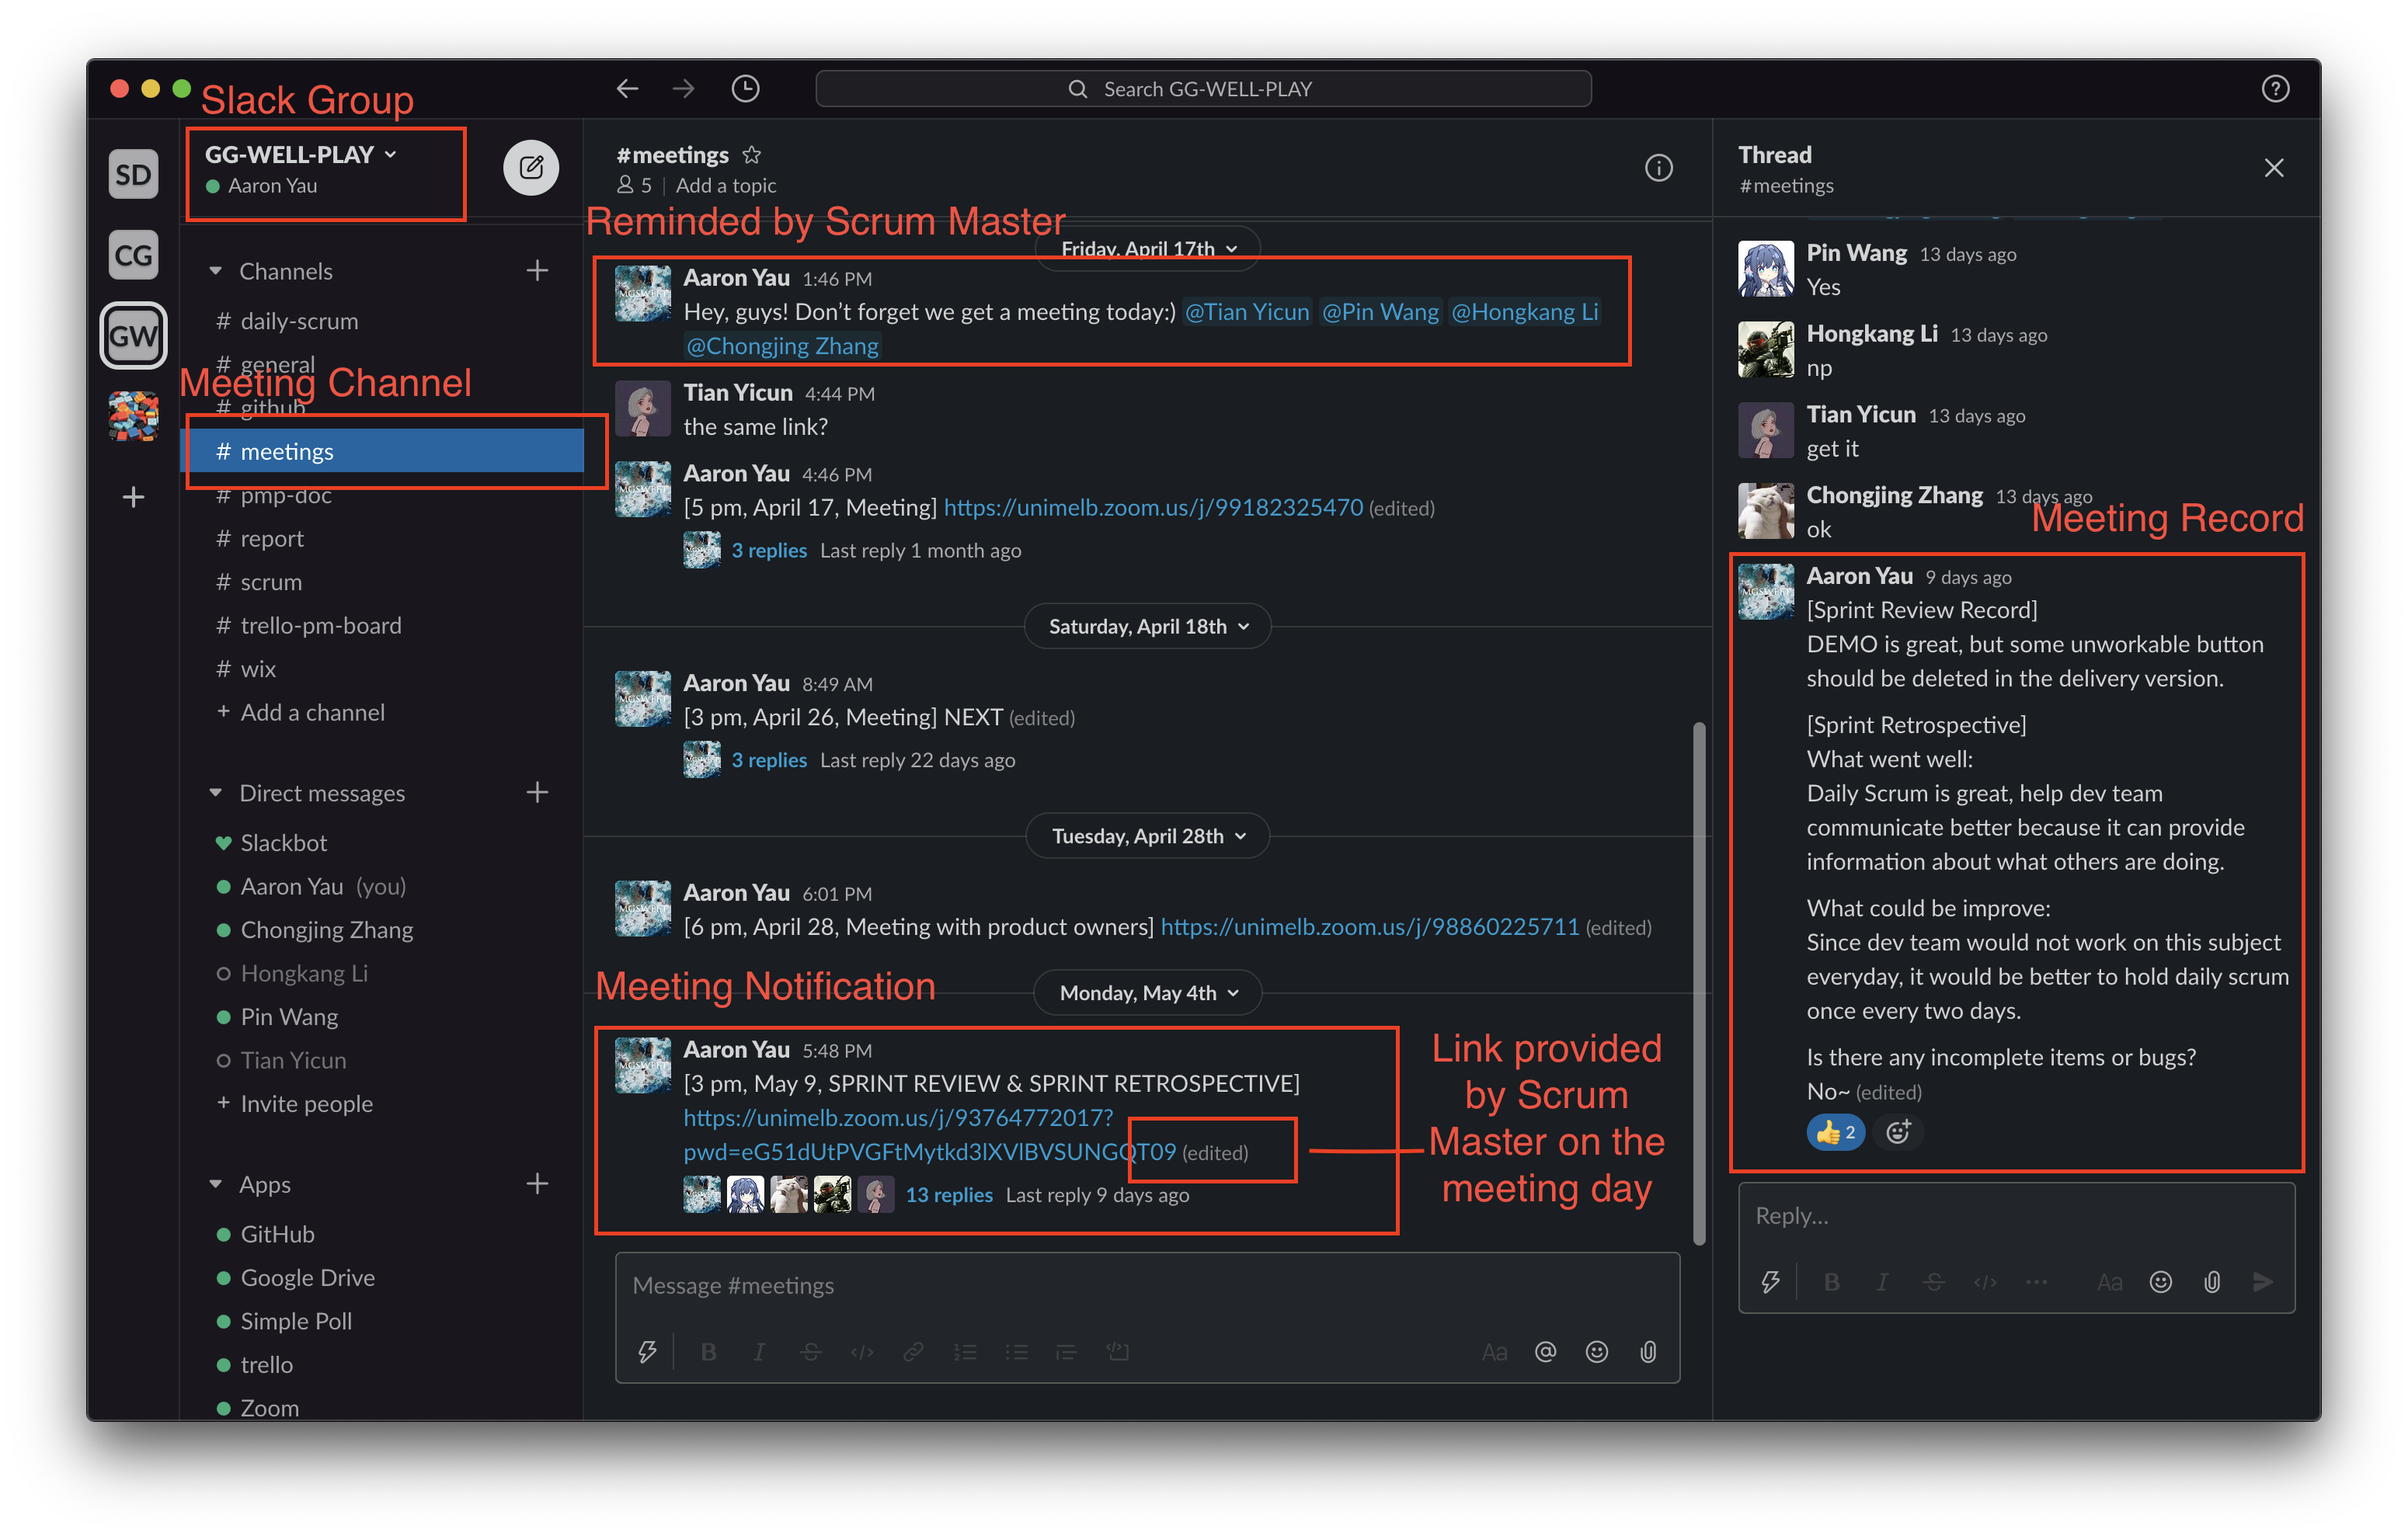
\includegraphics[width=\textwidth]{Figures/meeting.png}
\caption{Example of our Virtual Meeting Communication System}
\label{fig:meeting}
\end{figure}

Secondly, we use \textit{Trello} to help manage our Agile Board. Both the Project Backlog and the Sprint Backlog are managed on the Agile Board.

Furthermore, \textit{Github} is used to help enhance our teamwork and to manage our outcomes, such as the release of code and report.

According to the constraints of running a virtual team (Section \ref{sec:constraints}), we adjusted some of the communication processes in Scrum, and our communications matrix is shown in table \ref{tab:communicationMatrix}. 
\\

\begin{tabularx}{\linewidth}{%
  >{\raggedright\arraybackslash}p{1.5cm}%
  >{\raggedright\arraybackslash}p{2cm}%
  >{\raggedright\arraybackslash}X%
  >{\raggedright\arraybackslash}p{1.5cm}%
  >{\raggedright\arraybackslash}p{2cm}%
  >{\raggedright\arraybackslash}p{1.1cm}%
  >{\raggedright\arraybackslash}l}
  \toprule
  Processes & Stakeholder & Communication Objective & Format & Frequency & Owner & Importance
  \\
  \midrule
  Emergency Meeting
  & - Scrum Master
  \newline - Everyone in the team relative to the emergency meeting
  & To handle any unforseen emergency situation.
  & Virtual Meeting -- \textit{Zoom}; Formal Report
  & Anytime when needed
  & Scrum Master
  & High
  \\
  \midrule
  Project Planning Meeting
  & 
  - Scrum Master
  \newline - Product Owner
  \newline - Dev team
  \newline - Subject Matter Expert
  & Provide definition of the product backlog and provide a project plan for the whole project.
  & Virtual Meeting -- \textit{Zoom}; Formal Report
  & Weekly before the first sprint
  & Scrum master
  & High
  \\
  \midrule
  Sprint Planning Meeting
  & 
  - Scrum Master
  \newline - Product Owner
  & Provide Sprint Backlog, which selects high priority items from the Product Backlog that the Development Team can commit to delivering in a single Sprint.
  & Virtual Meeting -- \textit{Zoom}
  & At the beginning of each sprint:
  \newline - April, 27, 2020
  \newline - May, 11. 2020
  \newline - May, 25. 2020
  & Scrum master
  & High
  \\
  \midrule
  Daily Scrum
  & 
  - Scrum Master
  \newline - Product Owner
  \newline - Dev team
  & A short meeting used to start a day's work. Since we defined our features clearly, and every progress is shown in the Agile Board in \textit{trello}, we defined the importance of it to be medium.
  & Chat in the \textit{daily-scrum} channel of \textit{Slack}
  & Daily in the first sprint. In the second sprint, only held on:
  \newline - Monday
  \newline - Wednesday
  \newline - Friday
  & Scrum master
  & Medium
  \\
  \midrule
  Sprint Review
  & - Scrum Master
  \newline - Business Owner
  \newline - Product Owner
  \newline - Dev team
  & Show the demo of new features to Stakeholoders and get feedbacks from them.
  & Virtual Meeting -- \textit{Zoom}
  & At the end of each sprint:
  \newline - May, 8, 2020
  \newline - May, 22. 2020
  \newline - May, 30. 2020
  & Scrum master
  & Medium
  \\
  \midrule
  Sprint Retrospective
  & - Scrum Master
  - \newline - Business Owner
  - \newline - Product Owner
  - \newline - Dev team
  & An examination of what went well, what could be improved, etc. To make each Sprint more efficient and effective than the last.
  & Virtual Meeting -- \textit{Zoom}
  & At the end of each sprint
  \newline - May, 8, 2020
  \newline - May, 22. 2020
  \newline - May, 30. 2020
  & Scrum master
  & Medium
  \\
  \midrule
  Daily communication
  & - Anyone in the team
  & For exchanging information and better cooperation
  & Casual Chat on \textit{Slack} or personal \textit{Zoom} meeting.
  & Any working hours when needed
  & Anyone in the team
  & Low
  \\
  \bottomrule
  \\
  \caption{Communication Matrix}  
  \label{tab:communicationMatrix}
\end{tabularx}

\section{Risk Management}
\label{sec:riskManagement}
\subsection{Risk Impact Analysis Table}
\label{sec:riskImpactAnalysisTable}
We follow the following scoring rules to assess the impact of each risk:
\textit{(1) no impact; (2) minimal impact; (3) moderate impact; (4) severe impact; and (5) catastrophic impact;} The Risk Impact Analysis Table is shown in Table \ref{tab:riskImpactAnalysisTable}.

\begin{tabularx}{0.95\linewidth}{%
  >{\raggedright\arraybackslash}p{1cm}%
  >{\raggedright\arraybackslash}p{1.2cm}%
  >{\raggedright\arraybackslash}p{2cm}%
  ll%
  >{\raggedright\arraybackslash}X}
  \toprule
  Risk ID & Risk Type & Description & Probability & Impact & Justification\\
  \midrule
  1
  & Product
  & Design problem - The software developed by Wix has low scalability and is untransferable.
  & 60\%
  & 4
  & Although Wix can help quickly implement some basic functions, it may not be suitable for implementing the future enhancement of the project. There are many restrictions on creating a website on Wix. For example, the starter plan (\$5 per month) doesn't remove ads from the website, and there is no unlimited bandwidth or storage plan provided. You cannot build a high availability server in Wix. The site created by Wix is not transferrable.
  \\
  \midrule
  2
  & Business
  & Cancel orders maliciously or for no reason.
  & 3\%
  & 5
  & Malicious orders may cause unnecessary waste.  Some malicious buyers may intentionally create many orders and cancel them on the day of delivery. This kind of malicious actions may negatively affect the operation of the website and cause unnecessary loss. 
  \\
  \midrule
  3
  & Business
  & Email system or network system may fail.
  & 5\%
  & 2
  & If the email system or network system failed, the buyer would be unable to receive a confirming email after ordering. If clients were not able to receive feedback in time, they would not know whether their orders are confirmed or not. This situation may cause adverse effects on the user experience and cause unnecessary loss.
  \\
  \midrule
  4
  & Business
  & Service cancelation - Jess and James cannot deliver in time due to unforeseen circumstances.
  & 5\%
  & 1
  & Unforeseen circumstances like Jess and James getting sick or unnecessary travel ban may result in delivery cancelation. When they are unable to deliver, they have to provide reasons for their customer and cancel the order. Even though they may lose some money and customers may be disappointed, the impact of it would be small.
  \\
  \bottomrule
  \\
  \caption{Risk Impact Analysis Table}  
  \label{tab:riskImpactAnalysisTable}
\end{tabularx}

\subsection{Risk Register}
\begin{tabularx}{0.95\linewidth}{%
  >{\raggedright\arraybackslash}p{1cm}%
  >{\raggedright\arraybackslash}p{2cm}%
  >{\raggedright\arraybackslash}p{2cm}%
  >{\raggedright\arraybackslash}X%
  >{\raggedright\arraybackslash}p{2cm}%
  >{\raggedright\arraybackslash}p{2cm}}
  \toprule
  Risk ID & Trigger & Owner & Response & Response Strategy Type & Resources Required
  \\
  \midrule
  1
  & The new requirements proposed by Jess and James are confirmed by the development team that could not be implemented through Wix.
  & The development team
  & The development team can redevelop the whole system based on traditional web technics. Although it may take more time for the development team,  it can meet the needs of users. Also, keeping more reusable interfaces during development can help reduce the impact of this risk.
  & Mitigate or avoid 
  & The development team needs to keep more reusable interfaces during the development process.
  \\
  \midrule
  2
  & A user creates lots of orders in a short time and then cancels them without any reason. 
  & Jess and James
  & Limiting the number of times a user can cancel per week and limiting the time when the user cancels the order can help reduce the impact of this risk. For example, cancelation within 24 hours of the specified delivery time is not allowed. Also, customers would be asked to pay an advance deposit to reduce the economic loss caused by cancelation.
  & Mitigate
  & Jess and James need to spend effort to judge the reliability of the orders.
  \\
  \midrule
  3
  & Users complain that no confirmation email is sent to them.
  & Users(Jess \& James and customers)
  & If this risk occurs due to network failure, the system should be able to detect the user's network conditions and provide prompts automatically. The operation of the user to place an order is idempotent, which means that two identical operations will only operate once. If there is a problem with the function of auto-replying emails, the administrator of the maintenance system should be able to detect it in the background, the system is abnormal, and fix the bug in time.
  & Mitigate
  & The system needs to consume resources to detect the user's network environment and react to it.
  \\
  \midrule
  4
  & Jess or James is sick, or the government announced an unnecessary travel ban policy.
  & Jess and James
  & If an unnecessary travel ban policy is announced, Jess and James have to follow the rules and cancel their orders with an apology email sent to their customers. If the order cannot be delivered in time because the seller is sick or other assents, they can decide to hire another person to deliver or cancel their orders. It would be a trade-off between economic loss and user satisfaction loss.
  & Mitigate or accept
  & Hiring others for delivery would result in an economic loss, while cancelation of orders can bring negative effects to user experience.
  \\ 
  \bottomrule
  \\
  \caption{Risk Register}  
  \label{tab:riskRegister}
\end{tabularx}

\clearpage
\section{Technology}
\label{sec:technology}
The following are some technologies we researched for web development.
\begin{tabularx}{0.95\linewidth}{%l%
  >{\raggedright\arraybackslash}p{1.5cm}%
  >{\raggedright\arraybackslash}p{1.8cm}%
  >{\raggedright\arraybackslash}X%
  >{\raggedright\arraybackslash}X%
  >{\raggedright\arraybackslash}X}
  \toprule
  Name & Responsibility & Description & Pros & Cons \\
  \midrule
  Bootstrap
  & Front end framework
  & Bootstrap is a front-end framework that includes HTML and CSS based design templates and JavaScript plugins. It allows users to create responsive designs easily.
  & Easy to use and saves time; 
    Compatible with all browsers; 
    Responsive structures and styles;
  & Load time can be slow, file size can be huge; 
   All websites using Bootstrap look the same with out style customization;
  \\
  \midrule
  Foundation
  & Front end framework
  & Foundation is a front-end framework that is a collection of HTML, CSS and JS. It is a easy-to-use, powerful, and flexible framework for building web applications on any device.
  &  Fast development;  Adapt to all devices; Robust grid system;
  &  Community support is worse compare to Bootstrap; Need time to learn for beginners;
  \\
  \midrule
  Angular
  & Front end framework (JS)
  & Angular is a development platform for building web applications using TypeScript.
  & Component-based architecture allows reuse of components of UI, which is easy for writing tests; High performance; Fast development;
  & Difficult to manage components; Need time to learn for beginners; Lacks CLI documentation;
  \\
  \midrule
  React.js
  & Front end framework (JS)
  & React is a JavaScript library for building user interfaces. It can be used as the basis for developing web pages and mobile applications.
  & Components are modularized; Stable; Compatible with all browsers; Fast development;
  & Longer learning time than Angular; Lack of documentation; Less straightforward than pure JavaScript;
  \\
  \midrule
  Vue.js
  & Front end framework (JS)
  & Vue.js is an progressive, incrementally adoptable MVVM JavaScript framework for building user interfaces and single-page applications.
  & Clear documentation, simple to study; Small and fast; Components are modularized;
  & Too flexible that the codes are irregular; New framework, not very mature, has a smaller community;
  \\
  \midrule
  Java
  & Back end programming language
  & Java is a programming language that is class-based, object-oriented, and concurrent.
  & High-level language with simple syntax; Object-oriented programming allows reuse of codes; Supports multi-threading and distributed computing; Compatible for all platforms;
  & Slower than natively compiled languages; Less compact;
  \\
  \midrule
  PHP
  & Back end programming language
  & PHP is a server scripting language and a powerful tool for web development. It is fast, flexible and pragmatic that makes it easier to make dynamic and interactive web pages.
  & Compatible for all platforms; Easily embedded into HTML; High scalability; Large community;
  & Slower than other languages; Flexibility allows bad code;
  \\
  \midrule
  Python
  & Back end programming language
  & Python is an interpreted, high-level, general-purpose programming languages.
  & Easy to use and read; Multi-paradigm approach; Flexible;
  & Slower than natively compiled languages; Doesn't allow multi-threading;
  \\
  \midrule
  Django
  & Back end framework (Python)
  & Django is a Python-based high-level web framework follows MTV architectural pattern. It encourages rapid development and clean, pragmatic design.
  & Fast processing and developing; Scalable and flexible;
  & Not for smaller projects; Monolithic;
  \\
  \midrule
  Spring MVC
  & Back end framework (Java)
  & Spring MVC is a Java-based web framework that implements all the basic features of a core Spring framework like Inversion of Control and Dependency Injection.
  & Highly scalable and flexible; Use of modularity thus easy for testing; Large community;
  & Too complex, need time to learn for beginners; No clear guidelines;
  \\
  \midrule
  Express.js
  & Back end framework (Node.js)
  & Express is a minimal and flexible Node.js web application framework that provides a robust set of features for building web applications and APIs.
  & Fast development; Same language can be used to code front end; Simple; Flexible
  & Not for heavy projects;
  \\
  \midrule
  Wix
  & Web development platform
  & Wix is a popular cloud-based website builder. It provides an easy-to-use combination of powerful features that make it easy to build websites.
  & Flexible; Provides an app market; Easy to use; Massive template collection;
  & Loading is slow; Templates cannot be changed easily; Site cannot be transferred;
  \\
  \midrule
  Weebly
  & Web development platform
  & Weebly is a simple site builder with templates for great design. It allows the user to edit a website without any coding skills.
  & Massive template collection; Built-in support for e-commerce; Easy to use; Flexible;
  & Cannot add functionality not provided;
  \\
  \midrule
  WordPress
  & Web development platform
  & WordPress is a free and open source website builder. 
  & Powerful features; Scalability; Easy to use; Massive themes; A lot of free plugins;
  & Loading can be slow; Need to keep website updated; Doesn't support drag and drop;
  \\
  \bottomrule
  \\
  \caption{Available Web Development Technologies}  
  \label{tab:availableWebDevelopmentTechnologies}
\end{tabularx}
Among all technologies we researched above, we choose to use Wix content management system to build the website. Wix requires no coding skills or other usage of frameworks. It supports drag and drop to build web pages and provides a user-friendly UI to set the style of web components that integrates HTML and CSS from codes into user interfaces. And Wix also provides user-friendly UI to react to user actions with event handlers, this supports visualization of JavaScript. So far, Wix substitutes all front end languages or frameworks coding with user interfaces without any code. And Wix conceals the back end code in encapsulated apps, but also let users to implement customized logic using Node.js. Nonetheless, Wix offers a database operated by itself which also supports changes through graphical user interface. This database maintains the consistency of the usage of Wix platform, without extra database construction.

Compare to other website builders, Wix is more flexibly as it supports usage of Node.js to write customized backend code and take action when doing processes. And it already provides ready-made modules including online shop, user login, user permission management, and check out with credit card which can be used in developing the JJFresh website.

Take our project planning into consideration, we will need to implement all features of this website in 4 weeks. To complete the work on time, and not let it take too much time everyday as well, we want to be as efficient as possible, and also take use of the current existing web development tools to avoid building wheels. Nonetheless, we have the constraints that our development team members are not familiar with web development, no matter Wix or other frameworks and technologies.

By using Wix, we will save time of building and integrating the frameworks and adjusting the component properties with the help of visible user interface. And since we don't have much experience in web development, Wix's characteristic that it requires as least coding as possible is suitable us, and can help us focus on project management instead of catching up with the technology stacks. Therefore, we decided to use Wix to develop the website.

\section{Project Planning}
\label{sec:projectPlanning}
The SDLC of our project is Scrum. Since the key requirements for the initial development provided by Jess and James are fixed, a Fixed-Scope Release Planning would be used to plan our project.

\subsection{Product Backlog}
\label{sec:productBacklog}
The detail of product backlog is shown in Table \ref{tab:productBacklog}. \textit{Fabonacci sequence}\footnote{https://www.mountaingoatsoftware.com/blog/why-the-fibonacci-sequence-works-well-for-estimating} is used to provided relative estimation to both story point and value point.

The story points of different features are estimated by the development team and the Scrum master, based on the volume, risk, uncertainty and complexity of the features. We set the cost of the simplest feature (Edit admin account information) to 1 story point. And then estimate all other features' cost based on comparison with the simplest feature. 

The value points of the features are estimated by the product owners. We set the value of the least value feature (Edit admin account information) to 1 value point. And other features' values are estimated based on their relative value compared to the least value feature. 

BFTB Score is the abbreviate of the Bang-for-the-Buck\footnote{http://leftfoot.com.au/blog/struggling-with-relative-estimation-and-why-we-dont-use-time-watch-this} Score, which is a way of measuring how to get the most value in the shortest time. It is used to help assess the priority of the features. The BFTB Score is calculated by the formula below:
$$
  \text{BFTB Score} = \frac{\text{Value Point}}{\text{Store Point}}
$$

Initially, we define three milestones in our project. The first two milestones would be achieved at the end of the first sprint and at the end of the second sprint, respectively. Whether we would achieve the milestone depending on James and Jess's decision. Every milestone, we would release a runnable website to the market.
\begin{itemize}
\item The first milestone is to let the website go online without the function of purchase. The website can display all kinds of information about the products and provide the service of user registration. At the same time, the database is initially established to record the data of users and products.
\item The second milestone is to allow users to place orders to purchase products. After this milestone, sellers can view and modify user orders. Basic requirement testing has to be passed in this milestone.
\item The third milestone is to finish the future enhancement, which would not be considered in the initial development.
\end{itemize}

The features in Table \ref{tab:productBacklog} are ordered by their priority. The priorities are defined base on both the BFTB score and the development requirements. For example, even though the Database feature has a low BFTB score, because we can't record any data without it, its priority is still the highest.

Except for the three future user stories at the end of the product backlog table, all others are must-have stories because they are key requirements defined by Jess and James.
\begin{tabularx}{0.95\linewidth}{%
  l
  >{\raggedright\arraybackslash}p{3cm}%
  >{\raggedright\arraybackslash}X%
  p{1cm}p{1cm}p{1cm}
}
\toprule
Milestone & Feature & User Story & Story Point & Value Point & BFTB Score\\
\midrule
1
& Database
& As an admin, I need a database, so that I can store all the information of customers orders.
& 8
& 5
& 0.625
\\
\midrule
1
& Admin sign in and sign out
& As an admin, I want to provide my username and password, so that I can register an admin account.
& 2
& 2
& 1
\\
\midrule
1
& Manage product infomation
& As an admin, I want to manage product information, so that I can change the price or picture of my products.
& 5
& 3
& 0.6
\\
\midrule
1
& Browse product menu 
& As a customer, I want a menu that shows all the products, so that I can know what products are the website selling. 
& 8
& 5
& 0.625
\\
\midrule
1
& Customer sign up
& As customers, I want to sign up for the website, so that I can a member of the website.
& 2
& 2
& 1
\\
\midrule
1
& Customer sign in and sign out
& As customers, I should be able to sign in and sign out, so that I can manage my account and orders.
& 3
& 3
& 1
\\
\midrule
1
& Customer add and edit client information
& As customers, after login, I can add or edit my information like home address, user name, email address, and contact number.
& 2
& 3
& 1.5
\\
\midrule
2
& Add products to shopping cart
& As customers, after login, I can add or edit my information like home address, user name, email address, and contact number.
& 2
& 5
& 2.5
\\
\midrule
2
& Manage shopping cart
& As a customer, I want to manage my shopping cart, so that I can remove those I don't want or add some more products.
& 8
& 5
& 0.625
\\
\midrule
2
& Check out shopping cart
& As a customer, I want to choose the day and time for delivery, so that I can get the fruit on the right day.
& 8
& 5
& 0.625
\\
\midrule
2
& Cancel orders
& As a customer, I need to get the ability to cancel an order so that I can modify an order and then re-create.
& 2
& 2
& 1
\\
\midrule
2
& View and manage orders
& As an admin, I want the specific information of the user's order, so that I can packaging user orders.
& 8
& 5
& 0.625
\\
\midrule
2
& Register admin account
& As an admin, I need to get the ability to register for a new admin account, so that I can get more admin accounts if I need them.
& 1
& 1
& 1
\\
\midrule
2
& Edit admin account information
& As an admin, I may want to edit my admin account information, so that I can change the password.
& 1
& 1
& 1
\\
\midrule
3
& Add multiple bookings for the same slot
& As an admin, I want to add multiple bookings for the same slot in the future. So that I  can employ others to deliver boxes.
& 8
& 2
& 0.25
\\
\midrule
3
& Using AI to calculate delivery routes and times
& As an admin, I want to use AI technology to help me calculate an optimal route and time for delivery.
& 13
& 3
& 0.231
\\
\midrule
3
& Extended to allow for payment online.
& As an admin, I want to be paid online, so that I can save my time and improve the delivery efficiency.
& 13
& 3
& 0.231
\\
\bottomrule
\\
\caption{Product Backlog}  
\label{tab:productBacklog}
\end{tabularx}  

\subsection{Must-have Story Points}
Without calculating the features needed in the future, the total number of must-have story points is 60.
$$
SP_{total} = 60 \text{ (Story Point)}
$$

\subsection{Velocity Estimating (Re-estimate)}
There are two developers in our team. Since both of them are students, each of them can only spend about 1.2 to 3 hours a day on the project. They can work five days a week, so the total working hours of a week are 12 to 30 hours. We simply suppose each story point to be equivalent to one hour of working time. So the min velocity ($V_{min}$) for a two-week sprint is about 24 story points, and the max velocity ($V_{max}$) is about 60 story points. And by using the formula shown below, we can get our minimum and maximum number of sprints, which are 1 and 2.5, respectively. The velocity re-estimation burndown chart is shown in Figure \ref{fig:velocityEstimate}
$$
S_{min} = \frac{SP_{total}}{V_{max}}
\text{, } 
S_{max} = \frac{SP_{total}}{V_{min}}
$$
\begin{figure}[htp]
\centering
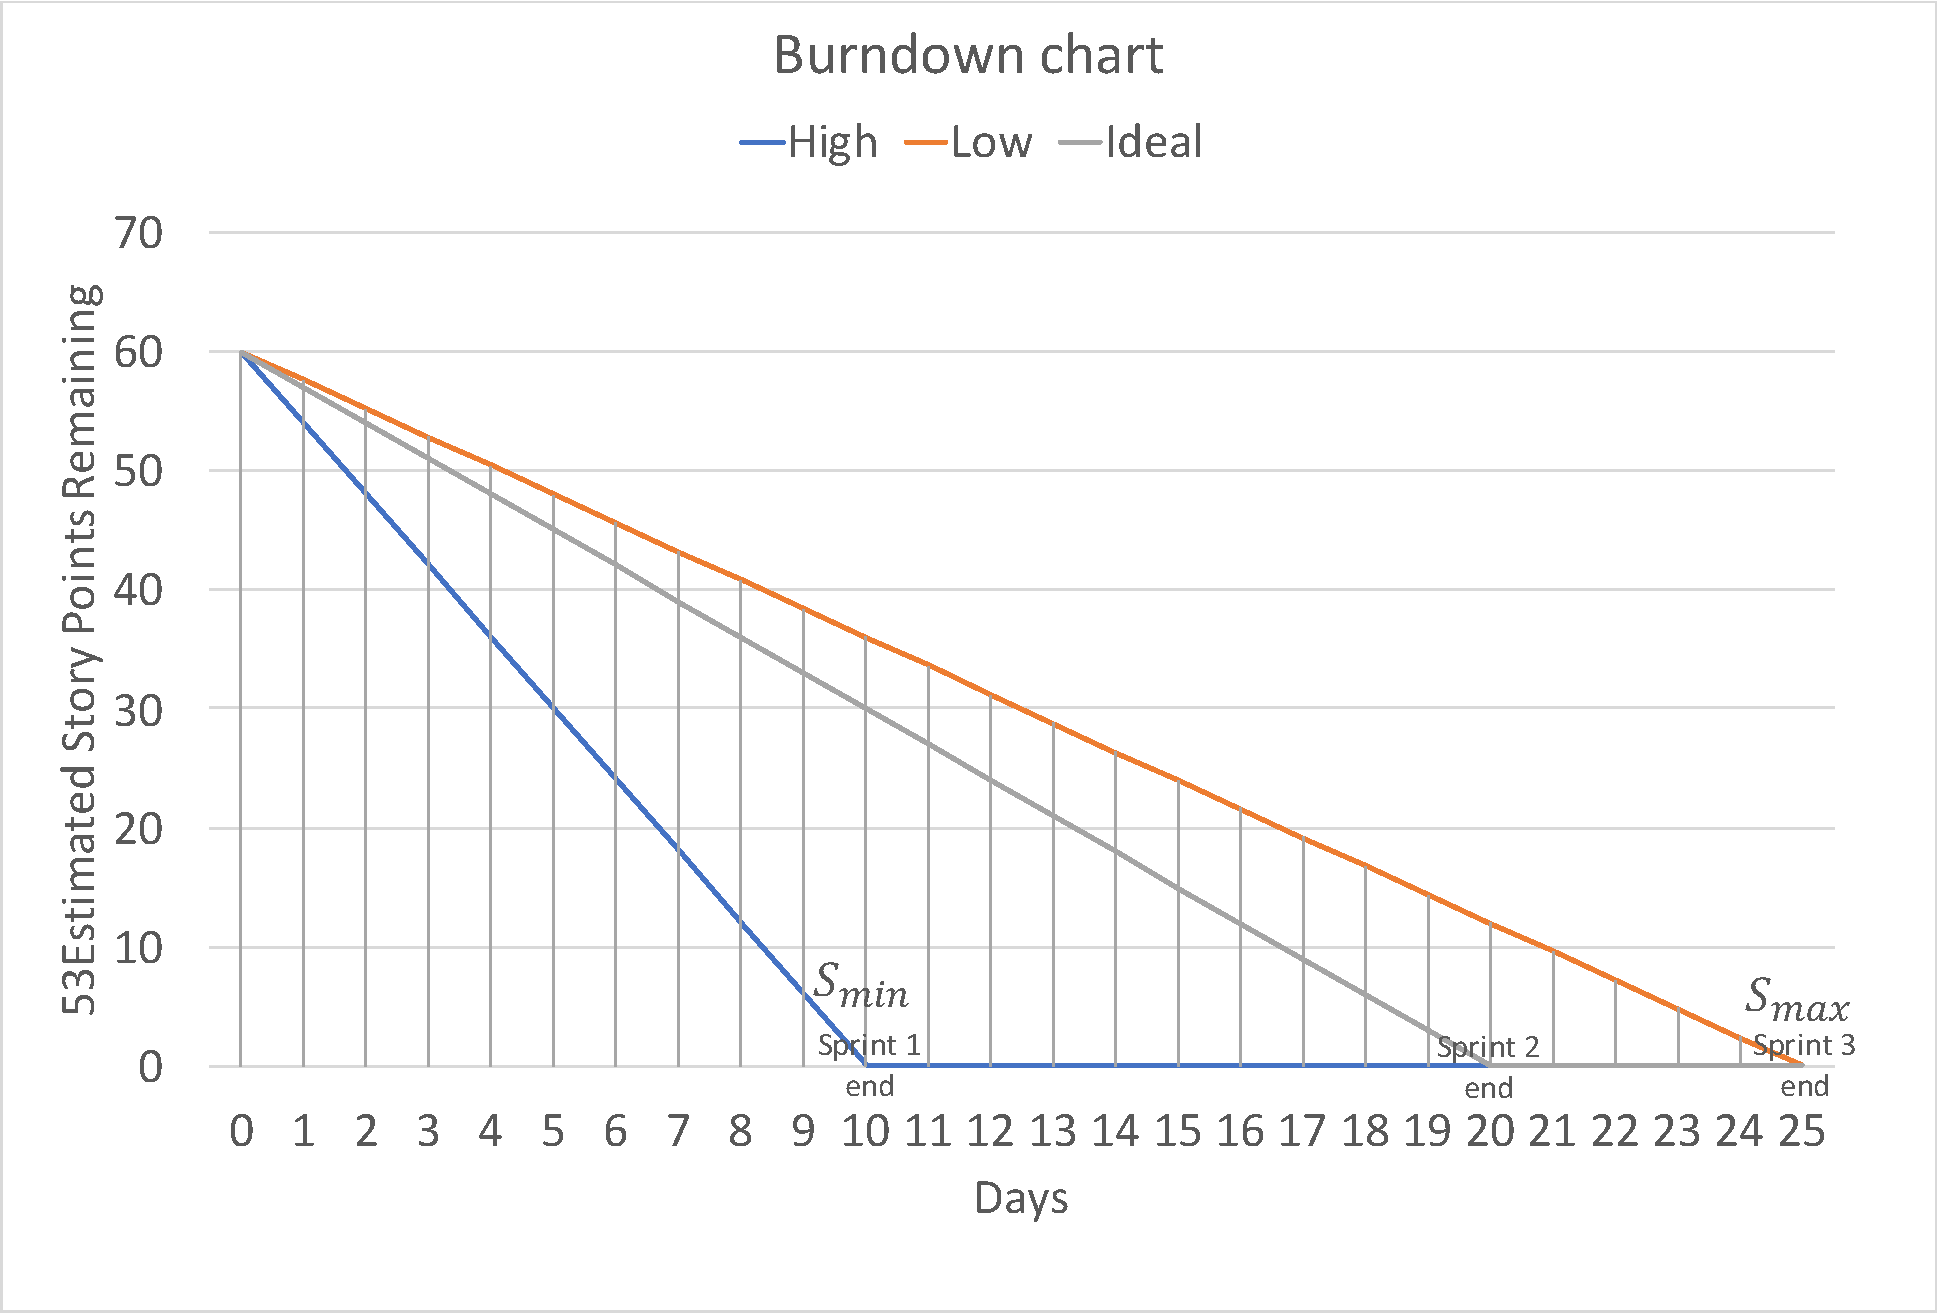
\includegraphics[width=0.9\textwidth]{Figures/velocityEstimate.pdf}
\caption{Velocity Re-estimation}
\label{fig:velocityEstimate}
\end{figure}

\clearpage
\subsection{Sprint Planning}
\subsubsection{Sprint Cycle}
\label{sec:sprintCycle}
The development phase of our project would start on \textbf{Monday, April 25}. Since the final delivery due date of the whole project is \textbf{June 1}, we decided to divide our development into three phases, each corresponding to a sprint.

The first phase is to let the website go online without the function of purchase. The website can display all kinds of information about the products and provide the service of user registration. At the same time, the database is initially established to record the data of users and products. The first sprint will last for two weeks, \textbf{from Monday, April 27 to Friday, May 8}. 

In the second phase, we need to realize the function that users place orders to purchase products, and sellers can view and modify user orders. Preliminary testing will also take place at this phase. The second sprint will last for two weeks, \textbf{from Monday, May 11 to Friday, May 22}.

The third stage is mainly based on user feedback to repair the vulnerability, carry out more tests and improve the existing functions. If some functions left over from the first two sprints are not implemented, they will also be solved in this sprint. As the project is nearing its end and there is less work left, the sprint in this phase will last only one week, \textbf{from Monday, May 25 to Friday, May 29.}

On \textbf{the first Monday of every sprint}, a Sprint Planning meeting would be held to select high priority items from the product backlog that the development team can commit to delivering in a single Sprint. The select itmes would be add to Sprint Backlog.

On \textbf{the last Friday of each sprint}, a Sprint Review meeting would be held to demonstrate the new features to Stakeholders, and a Sprint Retrospective meeting would be held to review the sprint.

A 15-minute Daily Scrum would be held \textbf{everyday} in the first sprint to start up the jobs. Everyone has to share what he/she did yesterday, what he/she plan to do, and what obstacles are slowing him/her.

\subsection{The First Sprint Plan}
As mention in Section \ref{sec:sprintCycle}, the main goal of the first sprint is to launch a webpage where customers can browse products. Considering both the BFTB Score, which is shown in Table \ref{tab:productBacklog} and the actual development needs, the Sprint Backlog of the first sprint is shown in table \ref{tab:firstSprintBacklog}. The total velocity and the delivery value of the first sprint is 30 story points and 25 value points, respectively. 
\\
\begin{tabularx}{0.95\linewidth}{%
  l%
  >{\raggedright\arraybackslash}p{2cm}%
  >{\raggedright\arraybackslash}X%
  >{\raggedright\arraybackslash}p{1cm}}
  \toprule
  Index & Feature & Tasks & Story Point\\
  \midrule
  1 
  & Database 
  & 1.Define the order model\textit{(1-hour)}; 2.Define the user information model\textit{(1-hour)}; 3.Define the admin information model\textit{(1-hour)}; 4.Create table and relation\textit{(2-hour)}; 5.Test\textit{(1-hour)}
  & 8
  \\
  \midrule
  2 
  & Browse product menu
  & 1.Provide a page for showing the list of the products\textit{(3-hour)}; 2.Show the types of the products\textit{(1-hour)}; 3.Show the price of the products\textit{(1-hour)}; 4.The price would change automatically\textit{(1-hour)}; 5.Show the pictures of products\textit{(1-hour)}.
  & 8
  \\
  \midrule
  3
  & Customer sign up
  & 1.Check whether the information of the user is valid\textit{(1-hour)}; 2.Add the user to the database and send a confirming email to the new member if valid\textit{(1-hour)}.
  & 2
  \\
  \midrule
  4
  & Customer sign in and sign out
  & 1.Sign in, check whether the user exist and whether the user's password correct\textit{(1-hour)}; 2.Sign out\textit{(1-hour)}; 3.Handle the problem of forgetting the user password (Allow password reset)\textit{(1-hour)}.
  & 3
  \\
  \midrule
  5
  & Customer add and edit client information
  & 1.Add and edit the name, email address, home address\textit{(1-hour)}; 2.Add and edit up to three multiple contact phone numbers\textit{(1-hour)}.
  & 2
  \\
  \midrule
  6
  & Manage product infomation
  & 1.Change the price of products\textit{(1-hour)}; 2.Change the pictures of products\textit{(1-hour)}; 3.Change the type of products\textit{(1-hour)}; 4.Add products\textit{(1-hour)}; 5.Delete products\textit{(1-hour)}.
  & 5
  \\
  \midrule
  7
  & Admin sign in and sign out
  & 1.Sign in\textit{(1-hour)}; 2. Sign out\textit{(1-hour)}.
  & 2
  \\
  \bottomrule
  \\
  \caption{The first Sprint Backlog (4.27 - 5.8)}  
  \label{tab:firstSprintBacklog}
\end{tabularx}

\subsection{The Second Sprint Plan}
\label{theSecondSprintPlan}
As mention in Section \ref{sec:sprintCycle}, the main goal of the second sprint is to allow users to place orders to purchase products. After this sprint, sellers can view and modify user orders. Basic requirement testing has to be passed in this sprint.

Following the feature development priority provided in Table \ref{tab:productBacklog}, the Sprint Backlog of the second sprint is shown in Table \ref{tab:secondSprintBacklog}. The total velocity and the delivery value of the first sprint is 30 story points and 24 value points, respectively. 

\begin{tabularx}{0.95\linewidth}{%
  l%
  >{\raggedright\arraybackslash}p{2cm}%
  >{\raggedright\arraybackslash}X%
  >{\raggedright\arraybackslash}p{1cm}}
  \toprule
  Index & Feature & Tasks & Story Pointt\\
  \midrule
  1
  & Add products to shopping cart
  & 1.Select size, type and amount of the products and add them to shopping cart.\textit{(2-hour)}
  & 2
  \\
  \midrule
  2
  & Manage shopping cart
  & 1.Select the items to pay\textit{(1-hour)}; 2.Change the amount of items\textit{(1-hour)}; 3.Delete items\textit{(1-hour)}; 4.View the price of the items selected\textit{(1-hour)}; 5.Provide a page to show all the items in the shopping cart\textit{(3-hour)}.
  & 8
  \\
  \midrule
  3
  & Check out shopping cart
  & 1.Choose a day and time for delivery.\textit{(1-hour)}. Only two bookings are allowed in a particular-hour.); 2.Send a confirming email to the customer\textit{(1-hour)}; 3.Show the day and time which is valid\textit{(2-hour)}; 4.Add an order to the user's order list\textit{(1-hour)}; 5.Handle synchronization problem\textit{(2-hour)}.
  & 8
  \\
  \midrule
  4
  & Cancel orders
  & 1.Cancel order\textit{(1-hour)}; 2.Send emails to both customer and admin\textit{(1-hour)}.
  & 2
  \\
  \midrule
  5
  & View and manage orders
  & 1.Confirm order\textit{(1-hour)}; 2.Order rank by date\textit{(1-hour)}; 3.Cancel order and provide reason\textit{(1-hour)}; 4.Provide a page to show order list with order information attach to it\textit{(4-hour)};
  & 8
  \\
  \midrule
  6
  & Register admin account
  & 1.Provide way for admin account registration\textit{(1-hour)}.
  & 1
  \\
  \midrule
  7
  & Edit admin account information
  & 1.Provide way for admin account information editing\textit{(1-hour)}.
  & 1
  \\
  \bottomrule
  \\
  \caption{The Second Sprint Backlog (May 11 - May 25)}  
  \label{tab:secondSprintBacklog}
\end{tabularx}  

\chapter{Project Execution, Monitoring and Control}
\label{chap:pe}
\section{Project Status: Friday Week 9}
\label{sec:ps1}
We finished all the features required in the initial development process on May 18, 2020. However, because the document has to be updated to version 1.1 before May 23, 2020, we can’t update artefacts generated by the second sprint review meeting and the second sprint retrospective to the document in this version. And we would decide whether the third sprint is needed in the comming sprint review. The online store can now be accessed on \textit{https://pinwang4.wixsite.com/website}. It is a beautiful and well designed site, with a user-friendly interface and all the features required in the initial development. A screenshot of the homepage is available in Figure \ref{fig:homepage}

We use a handy tool called \textit{Trello}\footnote{To join the Agile Board: https://trello.com/invite/b/ZqSHe7MR/9b942f7a393fb08379c206fb2064726a/spm-group-project} to manage our Agile Board. The feature cards in the Agile Board are set by the Scrum Master with tasks checklist defined inside them. Students in the development team would add themselves to a specific card and move the card to the \textit{TODO} list after the Daily Scrum standup meeting. A card is moved to \textit{DONE} list only if all the tasks in it are finished and pass tests. The total finish story points can be quickly check in the upper left corner of the \textit{DONE} list. By checking the card in the \textit{DONE} list, the Scrum Master can keep track of everyone’s contribution. A screenshot of the Agile Board system is shown in Figure 4.4.

The burndown chart is updated by the Scrum Master after every daily standup. By comparing the actual jagged line with the ideal schedule straight line, the Scrum Master can easily evaluate whether the development team is working efficiently, whether the sprint backlog can be finished on time and whether the progress of the project is hindered. Also, the burndown chart is used to re-estimate the velocity of the development team. 

In the first sprint, we held daily scrum standup meeting every workday. But since in the first sprint retrospective, our development team said that they might not work for this subject every day and the Daily Scrum Meeting is held too often. So we change the process to be held only on Monday, Wednesday and Friday. The daily scrum meetings are thought to be very useful since it not only can help our development team to improve their work efficiency but also let other knows what they are working on and what should be solved on a specific date. As mention in Section \ref{sec:constraints}, our team is facing some time difference problem. Daily Scrum were conducted via chat. We do it in the daily-scrum channel in \textit{Slack}. An example of how our daily scrum standup meeting system work is shown in Figure \ref{fig:dailyScrum} in Appendix B. The meeting record is shown in Table \ref{tab:dailyScrumStandupMeetingRecord} in Appendix B.

At the end of the first sprint, a sprint review is held to give a demo on the product to determine what are finished and what are not. The demo is excellent, and together we find out that some unworkable buttons should be deleted in the delivery version. After the sprint review, a sprint retrospective was held to help improve the team's efficiency. All the members in the development team thought the Daily Scrum is great. However, it is held too often since they have to learn other subjects. So, we decide to hold daily scrum standup only on Monday, Wednesday and Friday in the second sprint. The Record of the first pprint review and sprint retrospective can be found in \textit{https://www.youtube.com/watch?v=4slzV0LbUSY}.

\subsection{Process Related Artefacts}  
The Meeting Minutes can be found in Appendix A and the Daily Scrum Standup Meeting Record can be found in Appendix B. 

\textbf{Burndown Chart for the Whole Project}

\begin{figure}[htp]
\centering
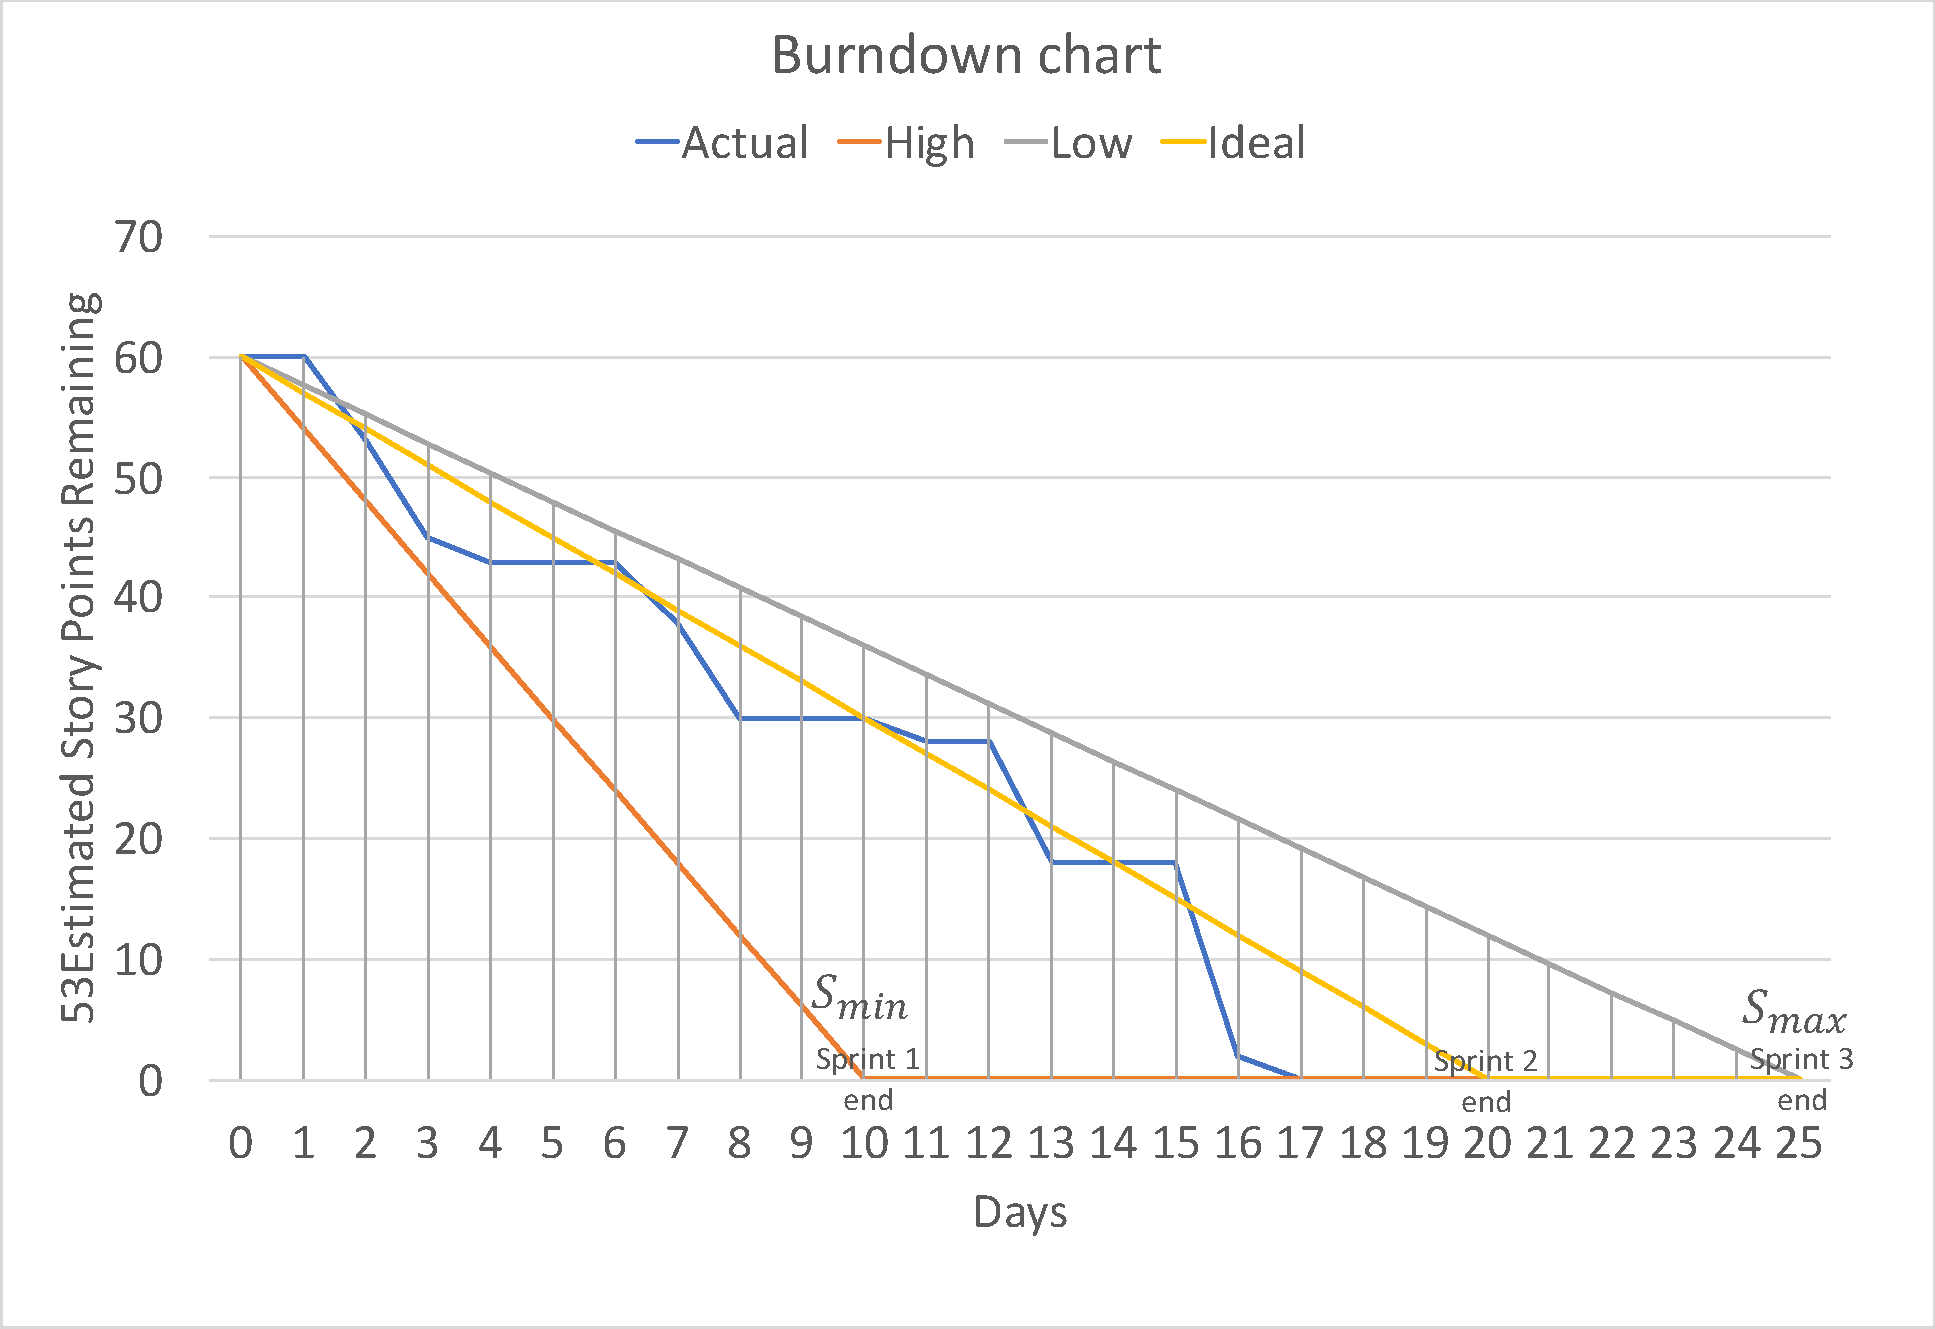
\includegraphics[width=\textwidth]{Figures/totalBurndown.pdf}
\caption{Burndown Chart of the Whole Project}
\label{fig:totalBurndown}
\end{figure}

\clearpage
\textbf{Burndown Chart for the First Sprint (April, 27 - May, 8)}
\begin{figure}[htp]
\centering
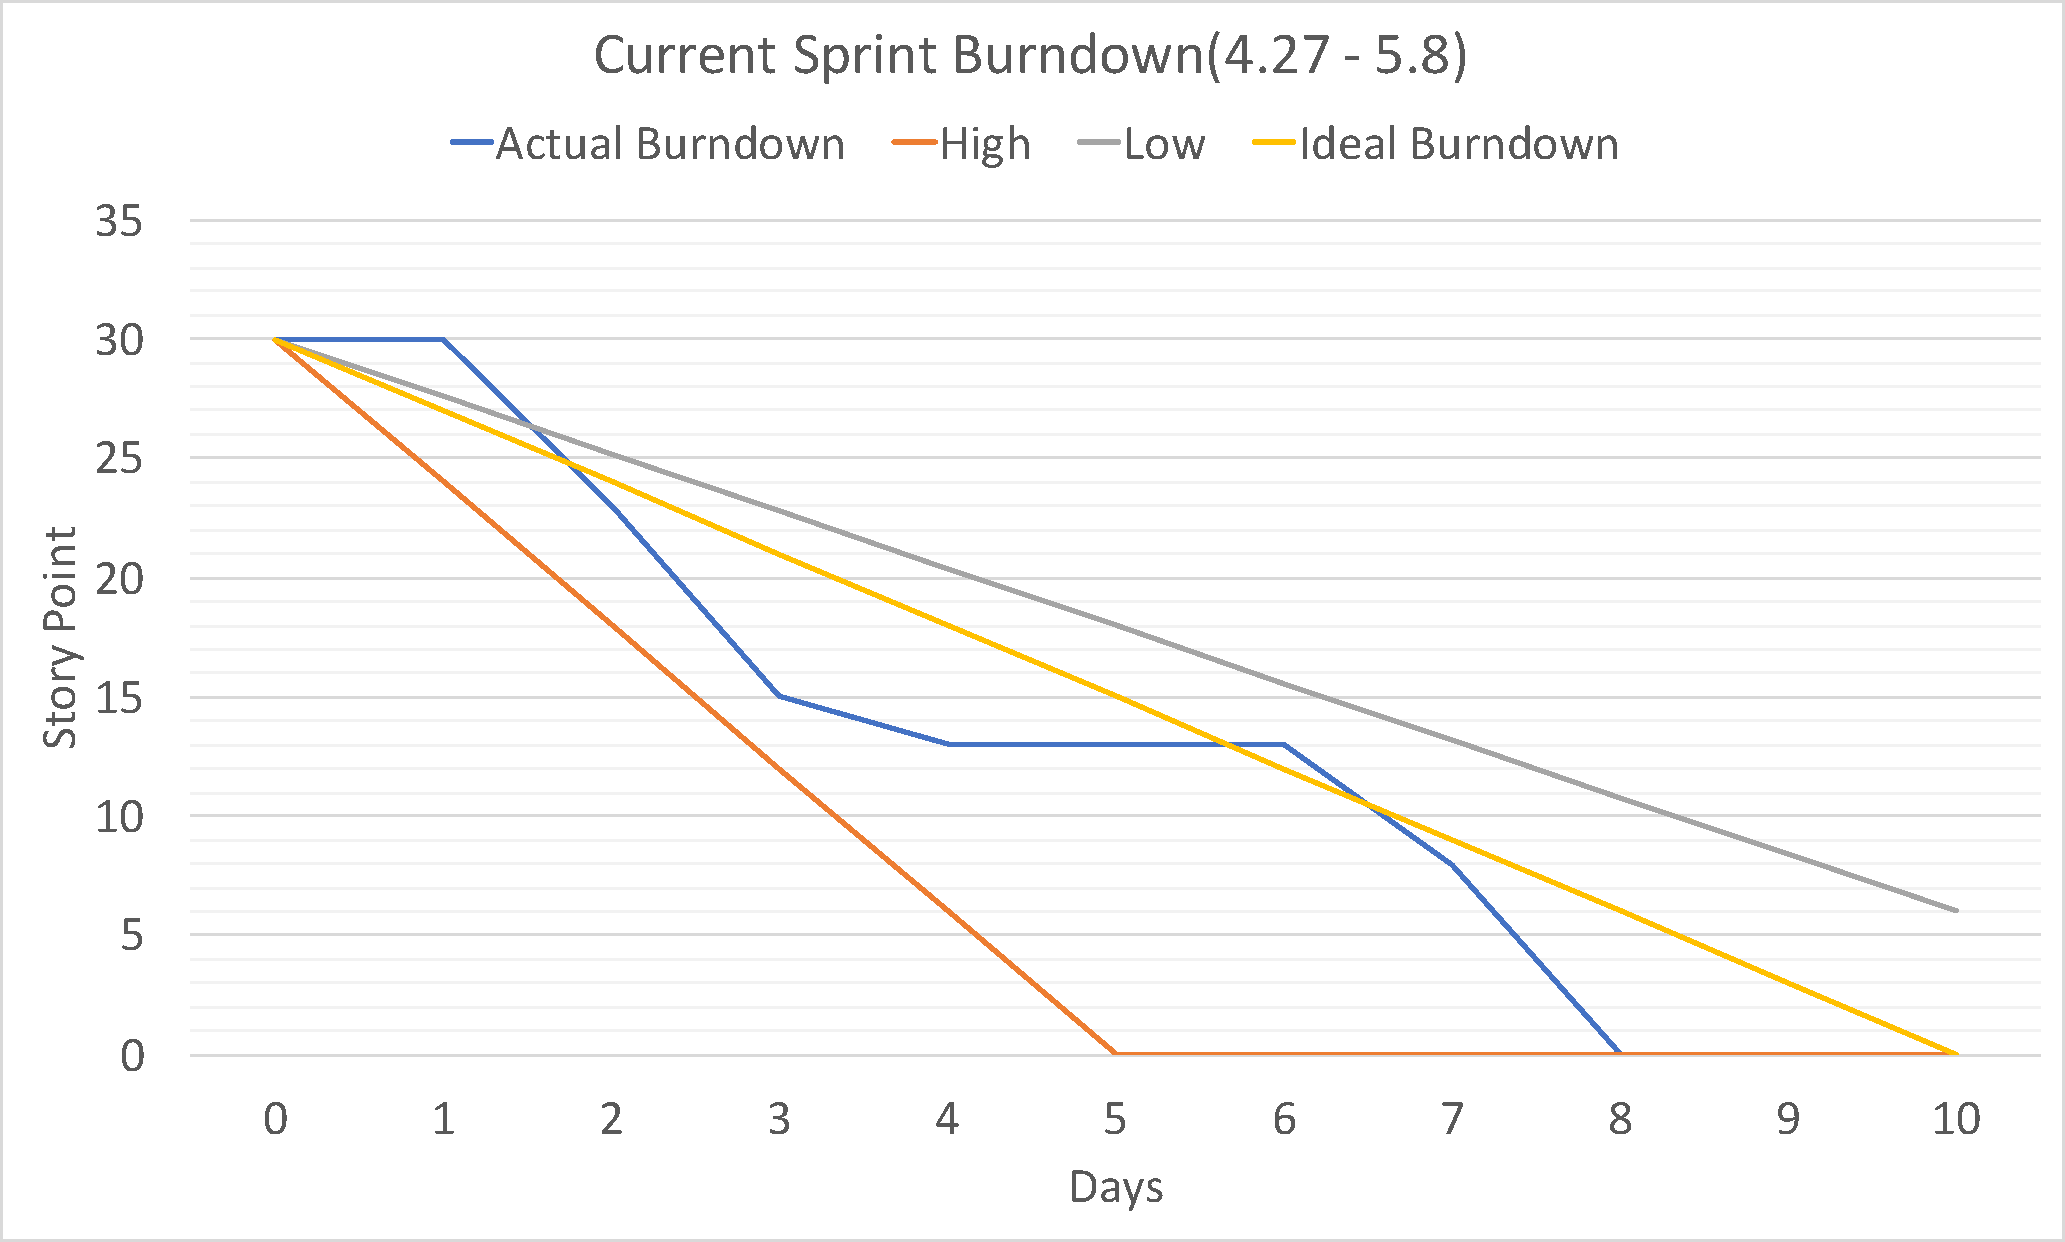
\includegraphics[width=0.65\textwidth]{Figures/sprint1Burndown.pdf}
\caption{Burndown Chart of the First Sprint}
\label{fig:sprint1Burndown}
\end{figure}
\\
\textbf{Burndown Chart for the Second Sprint (May, 11 - May, 22)}
\begin{figure}[htp]
\centering
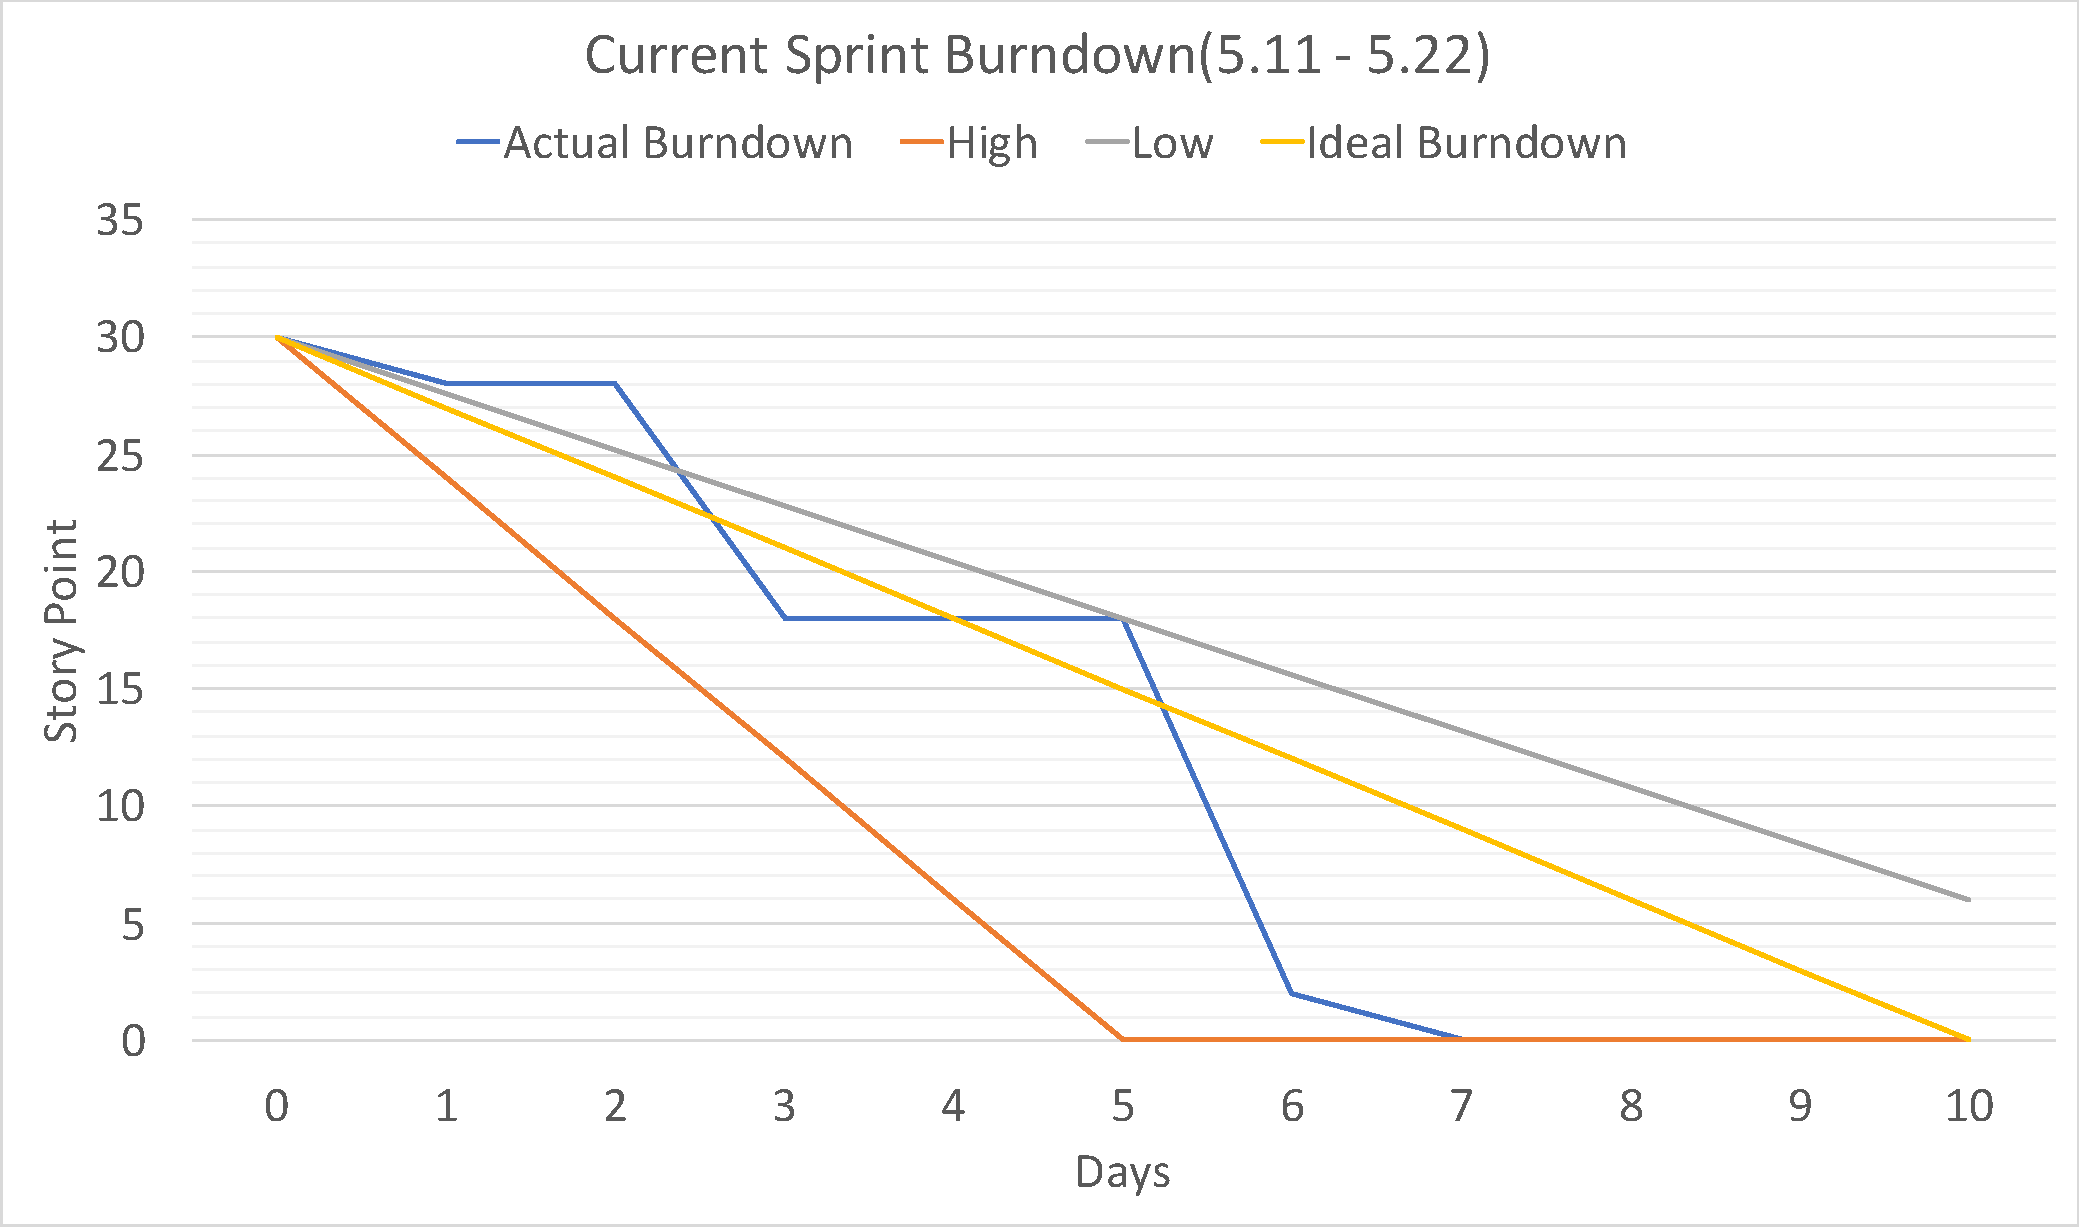
\includegraphics[width=0.65\textwidth]{Figures/sprint2Burndown.pdf}
\caption{Burndown Chart of the Second Sprint}
\label{fig:sprint2Burndown}
\end{figure}

\clearpage
\textbf{Agile Board}
\\
A handy tool called \textit{Trello} is used to manage our Agile Board. As present, all basic features have been realized. The Agile Board system is shown in Figure \ref{fig:agileBoard}:

\begin{figure}[htp]
\centering
\includegraphics[width=\textwidth]{Figures/agileBoard.png}
\caption{Agile Board}
\label{fig:agileBoard}
\end{figure}

%%%%%%%%%%%%%%%%%%%%%% Agenda %%%%%%%%%%%%%%%%%%%%%%%%%%%%%%%%
\clearpage
\textbf{Agenda}
\begin{tabularx}{0.95\linewidth}{%
  >{\raggedright\arraybackslash}p{0.15\linewidth}%
  >{\raggedright\arraybackslash}p{0.18\linewidth}%
  >{\raggedright\arraybackslash}p{0.12\linewidth}%
  >{\raggedright\arraybackslash}p{0.5\linewidth}
  }
  \toprule
  Date & Attendees & Format & Topic
  \\
  \midrule
  10 pm, April 12, 2020
  & Yicun Tian,\newline Hongkang Li,\newline Pin Wang,\newline Chongjing Zhang,\newline Zhangfeng Qiu
  & Virtual Meeting – Zoom
  & 
  1. Team creation and bonding.\newline
  2. Tasks Assignment.
  \\
  %%%%%%%%%%%%%%%%%%%%%%%%%%%%%%%%%%%%%%%%%%%%%%%%%%%
  \\
  \midrule
  5 pm, April 15, 2020
  & Yicun Tian,\newline Pin Wang,\newline Zhangfeng Qiu
  & Virtual Meeting – Zoom
  & 
  1. Initial project manage planing document job assignment.
  \\
  %%%%%%%%%%%%%%%%%%%%%%%%%%%%%%%%%%%%%%%%%%%%%%%%%%%
  \midrule
  5 pm, April 17, 2020
  & Yicun Tian,\newline Hongkang Li,\newline Pin Wang,\newline Chongjing Zhang,\newline Zhangfeng Qiu
  & Virtual Meeting – Zoom
  & 
  1. Requirement Breakdown.\newline
  2. User Story definition.\newline
  3. Product backlog definition.\newline
  4. User point and value point estimation.\newline
  5. Feature tasks break down.
  \\
  %%%%%%%%%%%%%%%%%%%%%%%%%%%%%%%%%%%%%%%%%%%%%%%%%%%
  \midrule
  3 pm, April 26, 2020
  & Yicun Tian,\newline Hongkang Li,\newline Pin Wang,\newline Chongjing Zhang,\newline Zhangfeng Qiu
  & Virtual Meeting – Zoom
  & 
  1. Discuss risks of the project.\newline
  2. Discuss stake holders of the project.\newline
  3. Decide the process we would go through in our first Sprint.\newline
  4. First Sprint Planning.
  \\
  %%%%%%%%%%%%%%%%%%%%%%%%%%%%%%%%%%%%%%%%%%%%%%%%%%%
  \midrule
  6 pm, April 28, 2020
  & Yicun Tian,\newline Zhangfeng Qiu
  & Virtual Meeting – Zoom
  & 
  1. Meeting with Subject Matter Experte -- Rajesh Chittor
  \\
  %%%%%%%%%%%%%%%%%%%%%%%%%%%%%%%%%%%%%%%%%%%%%%%%%%%
  \midrule
  3 pm, May 9, 2020
  & Yicun Tian,\newline Hongkang Li,\newline Pin Wang,\newline Chongjing Zhang,\newline Zhangfeng Qiu
  & Virtual Meeting – Zoom
  & 
  1. SPRINT REVIEW \newline 
  2. SPRINT RETROSPECTIVE
  \\
  %%%%%%%%%%%%%%%%%%%%%%%%%%%%%%%%%%%%%%%%%%%%%%%%%%%
  \midrule
  15-minute every workday (April, 27 - May, 8)
  & Yicun Tian,\newline Hongkang Li,\newline Pin Wang,\newline Chongjing Zhang,\newline Zhangfeng Qiu
  & Casual Chat on Slack
  & 
  The first sprint Daily Scrum Standup:
  \begin{enumerate}
    \item What the development team did yesterday.
    \item What the development team plan to do today.
    \item Block on the way.
  \end{enumerate}
  \\
  %%%%%%%%%%%%%%%%%%%%%%%%%%%%%%%%%%%%%%%%%%%%%%%%%%%
  \midrule
  15-minute, on Monday, Wednesday, Friday (May, 11 - May, 22)
  & Yicun Tian,\newline Hongkang Li,\newline Pin Wang,\newline Chongjing Zhang,\newline Zhangfeng Qiu
  & Casual Chat on Slack
  & 
  The second sprint Daily Scrum Standup
  \begin{enumerate}
    \item What the development team did in the last two day.
    \item What the development team plan to do today and tomorrow.
    \item Block on the way.
  \end{enumerate}
  \\
  \bottomrule
  \\
  \caption{Agenda}  
  \label{tab:agenda}
\end{tabularx}
%%%%%%%%%%%%%%%%%%%%%%%%%%%%%%%%%%%%%%%%%%%%%%%%%%%%%%

\textbf{The First Sprint Review \& Sprint Retrospective Record (May, 8, 2020)}
\\
The record of these two meetings can be found on \textit{https://www.youtube.com/watch?v=4slzV0LbUSY}.

In the sprint review, the development team give a presentation to show all the features finished in the first sprint. The Scrum Master and the Product Owners provide reviews for the product. We held the meeting in zoom. From the demo, we find out that there are some unworkable buttons which should be deleted in the delivery version. And after a little change based on the reviews, we release our first product to the market.

In the sprint retrospective, we discuss what went well in the first sprint. All the member in the development team thinks Daily Scrum is great. It helps the development team communicate better because it can provide information about what others are doing. When it comes to the "what could be improved" part, we decide to hold daily scrum standup only on Monday, Wednesday and Friday. This is because the development team would not work on this subject every day.

\subsection{Product Related Artefacts}
\textbf{The status of the product}
\\
We have finished all the features required in the initial development process. The online store website can be accessed now on \textit{https://pinwang4.wixsite.com/website}. A screenshot of the homepage is shown in Figure \ref{fig:homepage}. The online store website is beautiful and well designed, with a user-friendly interface and all the features required in the initial development. The product design can be found in Appendix C. The use cases and user stories of the product is shown in Table \ref{tab:productBacklog} in Section \ref{sec:productBacklog}, which would not be shown again here. The detail of the features completed in each sprint can be checked in Section \ref{sec:sprintCycle}. Also the completed features detail can be check in our Agile Board in \textit{Trello}, which is shown in Figure \ref{fig:doneFeature}. For a quick look, a completed feature lists (detailed tasks breakdown would not be included here) is provided below:
\\
\begin{itemize}
  \item Milestone 1 -- let the website go online without the function of purchase. The website can display all kinds of information about the products and provide the service of user registration. At the same time, the database is initially established to record the data of users and products.
  \begin{enumerate}
    \item Datebase
    \item Browse product menu
    \item Customer sign up
    \item Customer sign in and sign out
    \item Customer add and edit client information
    \item Admin manage product infomation
    \item Admin sign in and sign out
  \end{enumerate}
  \item Milestone 2 -- Allow users to place orders to purchase products. After this milestone, sellers can view and modify user orders. Basic requirement testing has to be passed in this milestone.
  \begin{enumerate}
    \item Customer add products to shopping cart
    \item Customer manage shopping cart
    \item Customer check out shopping cart
    \item Customer cancel orders
    \item Admin view and manage orders
    \item Register admin account
    \item Edit admin account information
  \end{enumerate}
\end{itemize}

\begin{figure}[htp]
\centering
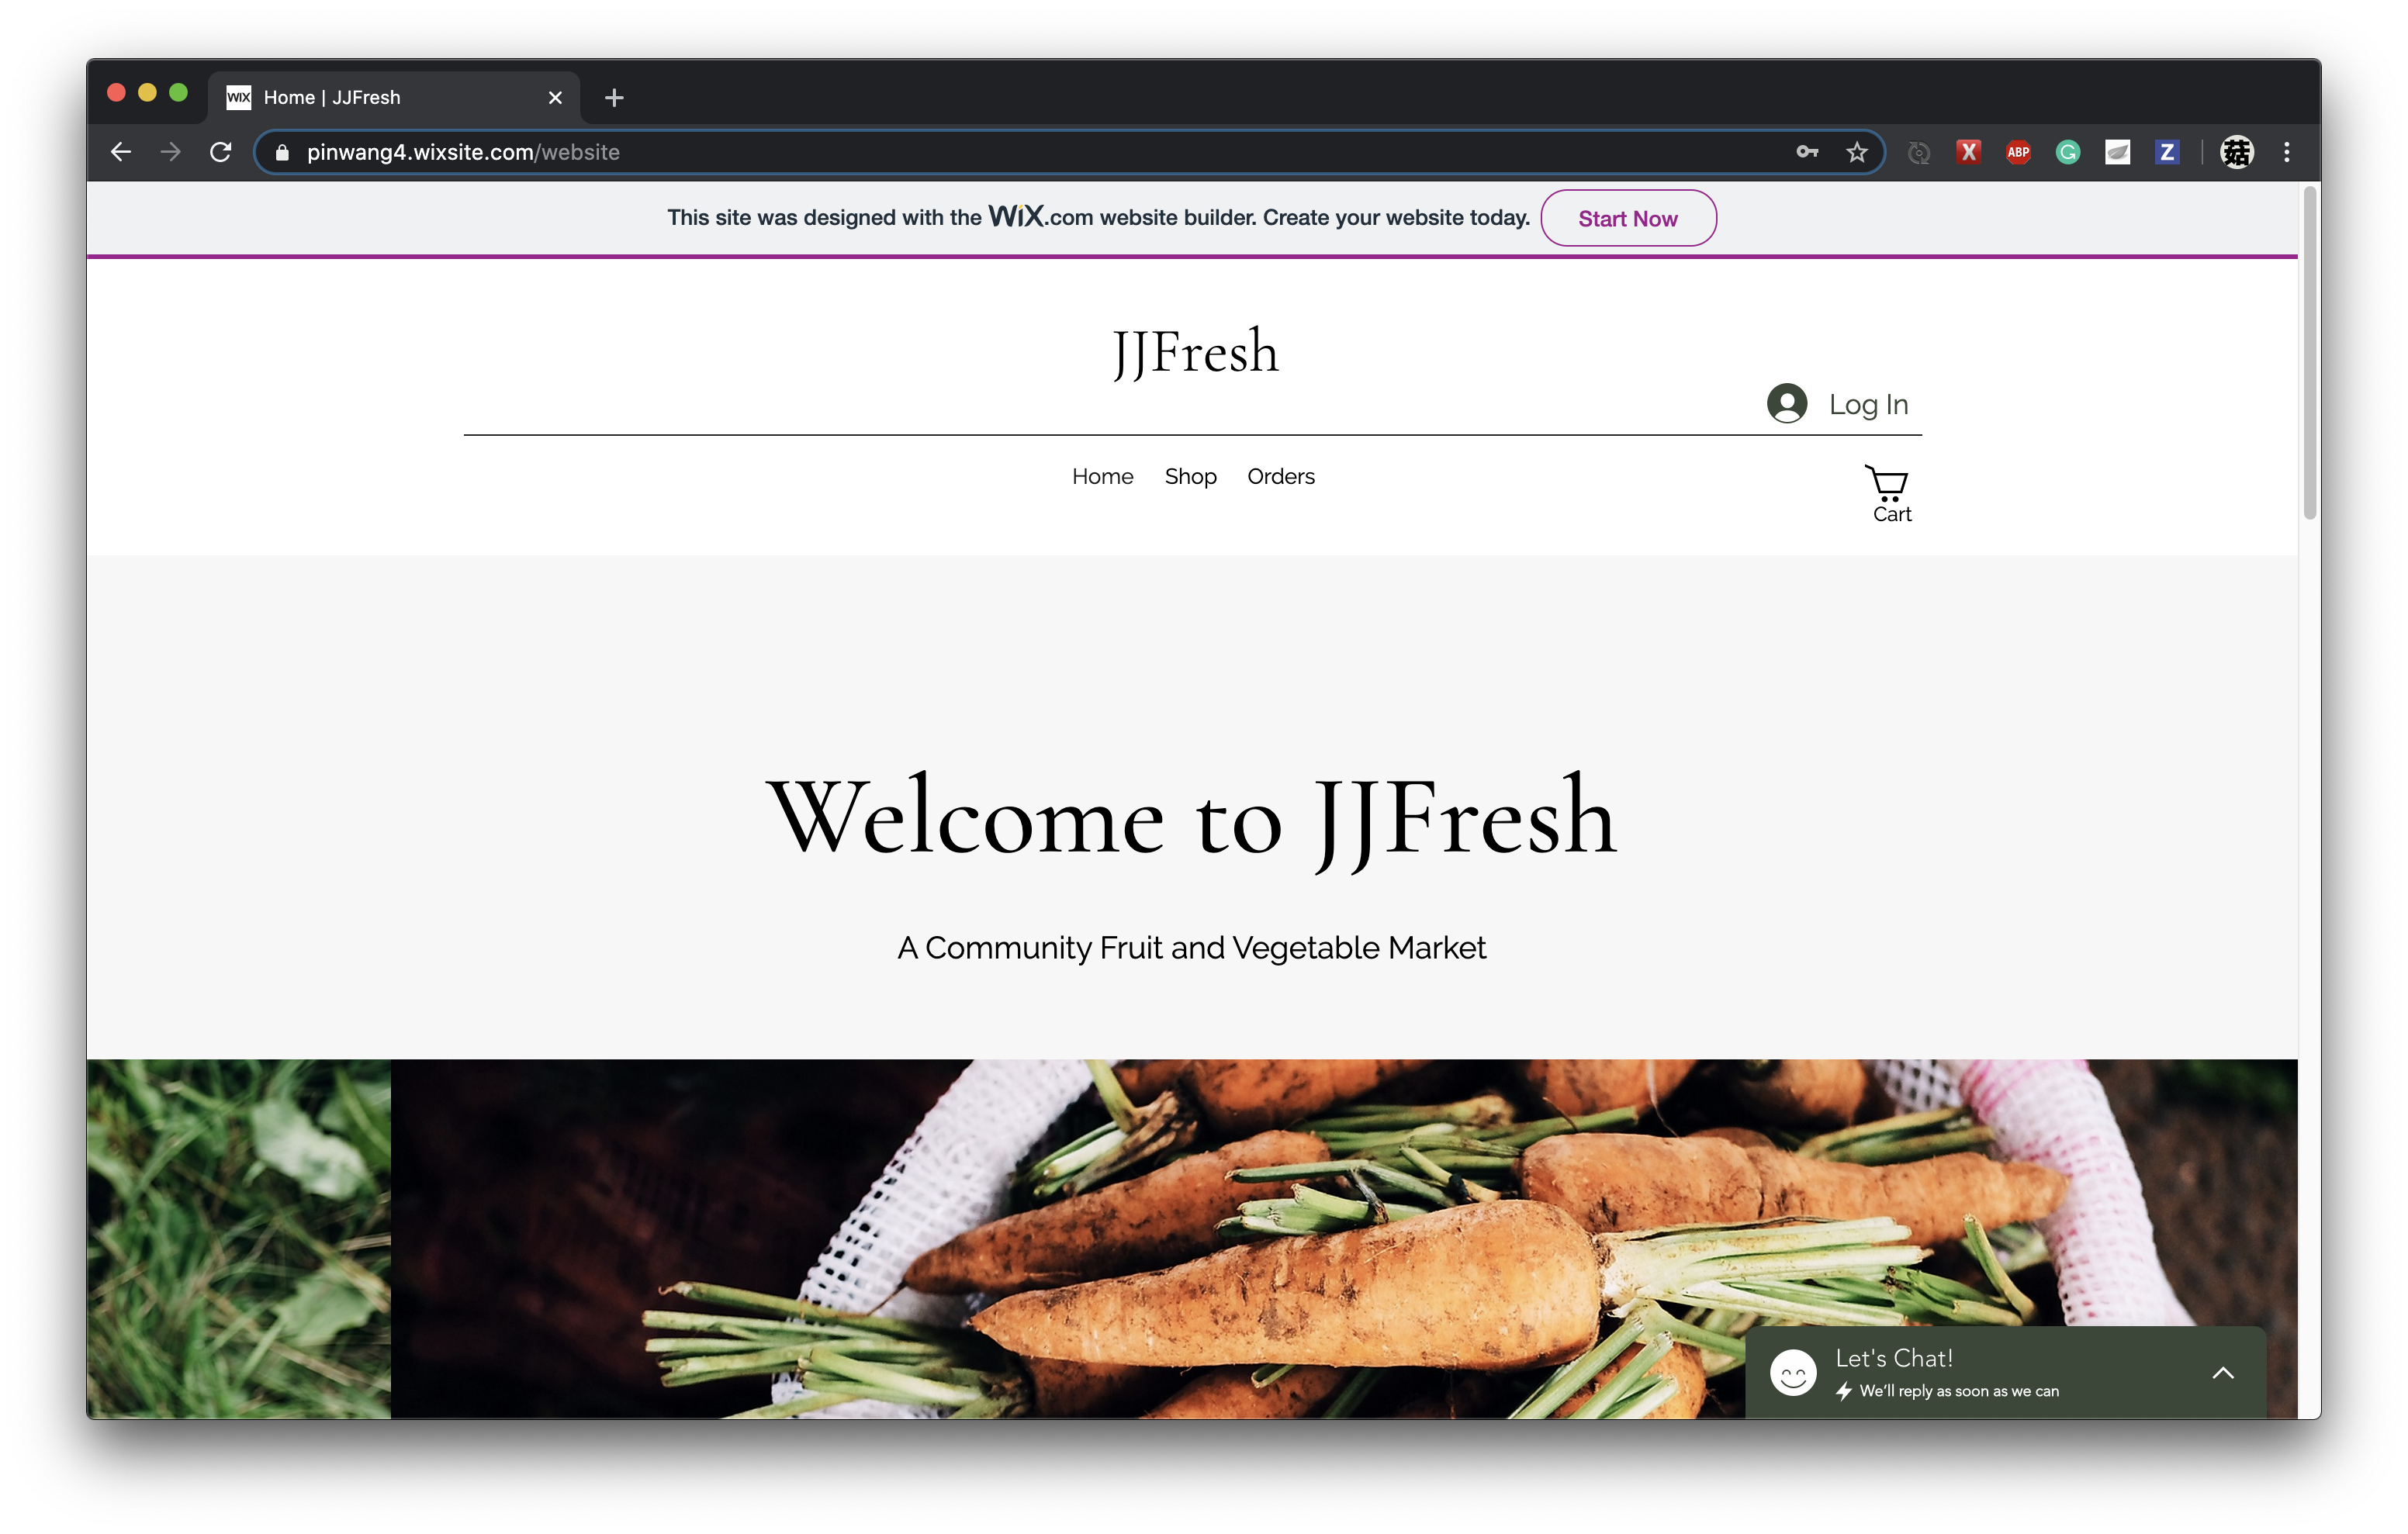
\includegraphics[width=\textwidth]{Figures/homepage.png}
\caption{Homepage of the online store}
\label{fig:homepage}
\end{figure}

\begin{figure}[htp]
\centering
\includegraphics[width=\textwidth]{Figures/doneFeature.png}
\caption{Done list in the Agile board}
\label{fig:doneFeature}
\end{figure}

\clearpage
\subsection{Risk Monitoring and Control}
After the product owner simulated the use of this system, risk 3 occurred.

Team member Tian Yicun simulates Jess and James for order processing and merchandising, and team member Li Hongkang simulates multiple users for shopping. This risk was detected after users frequently placed orders and canceled orders for no reason.

Our team used pre-defined solutions to alleviate the risk to a certain extent. The specific operations are as follows. When the problem was discovered by Tian Yicun, Jess and James, she believed that the development team should add some functions as pre-defined. For example, when the same user frequently cancels orders withour reason, the number of orders he can cancel should be limited to one week. The development team currently sets the number of cancelled orders to 3. On the other hand, if the user orders a large number of vegetables Fruit, assuming that the total value exceeds 50 AUD, she should limit the time he can order, for instance, within 24 hours after placing the order, it can be cancelled.

After using the system with the above two functions added in the second simulation, they found that the risk occurrence rate was reduced, and the loss was within an estimated range. Therefore, the risk is reasonably controlled.

In addition, after discussion, we discovered a new risk, the specific definition and control are as follows:

\begin{tabularx}{0.95\linewidth}{%
  l%
  >{\raggedright\arraybackslash}p{1cm}%
  >{\raggedright\arraybackslash}p{3cm}%
  >{\raggedright\arraybackslash}p{2cm}%
  >{\raggedright\arraybackslash}p{1cm}%
  >{\raggedright\arraybackslash}p{5cm}}%
  \toprule
  Risk ID & Risk Type & Description & Probability & Impact & Justification\\
  \midrule
  5
  & Business
  & Problems with suppliers, resulting in short supply of goods.
  & 40
  & 3
  & Because of the current impact of coronaviruses, the transportation and collection of vegetables and fruits are a serious problem. If the transportation time is too long, it will cause a shortage of supply. Besides many vegetables and fruits are susceptible to damage or rot due to bumps. If they do not pay attention to protection during transportation, the goods received by Jess and James may have quality problems,which will cause them to fail to complete the order on time and cause a certain economic loss.
  \\
  \bottomrule
  \\
  \label{Risk Monitor 1}
\end{tabularx}


\begin{table}
\begin{tabularx}{0.95\linewidth}{%
  l%
  >{\raggedright\arraybackslash}p{2cm}%
  >{\raggedright\arraybackslash}p{2cm}%
  >{\raggedright\arraybackslash}p{6cm}%
  >{\raggedright\arraybackslash}p{2cm}%
  >{\raggedright\arraybackslash}p{3cm}}%
  \toprule
  Risk ID & Trigger & Owner & Response & Response Strategy Type & Resources Required\\
  \midrule
  5
  & Suppliers are short of goods or have quality problems
  & Jess and James
  & Jess and James should find at least two suppliers. If one of them has problems, they can buy more from the other, so as to ensure the sufficient quantity of goods. In addition, they need to plan the purchase time reasonably so as not to be affected by the long transportation time.
  & Mitigate
  & Jess and James need to pay more attention to the situation of coronavirus and plan to purchase at least one week.
  \\
  \bottomrule
  \\
  \label{Risk Monitor 2}
\end{tabularx}
\end{table}



% \section{Project Status: Friday week 10}
% \subsection{Process Related Artefacts}
% \subsection{Product Related Artefacts}
% \subsection{Risk Monitoring and Control}
% \section{Project Status: Friday week 10}
% \subsection{Process Related Artefacts}
% \subsection{Product Related Artefacts}
% \subsection{Risk Monitoring and Control}

\chapter*{Appendix A: Team GGWELLPLAY Meeting Minutes}
\addcontentsline{toc}{chapter}{Appendix A: Team GGWELLPLAY Meeting Minutes}
%%%%%%%%%%%%%%%%%%%%%%%%%%%%%%%%%%%%%%%%%%%%%%%%%%%%%%%%%%%%
\section*{Meeting 1}
\subsection*{Opening}
The regular meeting of the GGWELLPLAY was opened at 10 pm on April 12, 2020 in \textit{Zoom}.

\subsection*{Present}
Yicun Tian, Hongkang Li, Pin Wang, Chongjing Zhang, Zhangfeng Qiu

\subsection*{Absent}
None

\subsection*{Approval of agenda}
The agenda was unanimously approved as distributed.

\subsection*{Approval of minutes}
The minutes of the previous meeting were unanimously approved as distributed.

\begin{tabularx}{0.95\linewidth}{%
  >{\raggedright\arraybackslash}p{0.1\linewidth}
  lll%
  >{\raggedright\arraybackslash}X
  }
  \toprule
  Task & Estimated Time & Actual Time & Completed & Comment \\
  \midrule
  Team creation and bonding.
  & 30min 
  & 35min
  & Yes
  & The role of each person was defined
  \\
  \midrule
  Tasks Assignment.
  & 60min 
  & 100min
  & Yes
  & Takes longer time. Chongjing and Hongkang would be in the dev team and find out the technology/framework we would use.(Take a look at whether we can finish the job on Wix.com);We decided to use SCRUM as the SDLC of the project. Yicun, Pin, Aaron would figure what should we do during a SCRUM process and provide a draft for the PMP version 1.0. 
  \\
  \bottomrule
\end{tabularx}

\subsection*{Next meeting}
The next general meeting will be at 5 pm on April 15, 2020 in \textit{Zoom}.

\subsection*{Minutes submitted by:} 
Yicun Tian

\subsection*{Approved by:} 
Zhaofeng Qiu

%%%%%%%%%%%%%%%%%%%%%%%%%%%%%%%%%%%%%%%%%%%%%%%%%%%%%%%%%%%%
\clearpage
\section*{Meeting 2}
\subsection*{Opening}
The regular meeting of the GGWELLPLAY was opened at 5 pm, on April 15, 2020 in \textit{Zoom}.

\subsection*{Present}
Yicun Tian, Pin Wang, Zhangfeng Qiu

\subsection*{Absent}
None

\subsection*{Approval of agenda}
The agenda was unanimously approved as distributed.

\subsection*{Approval of minutes}
The minutes of the previous meeting were unanimously approved as distributed.

\begin{tabularx}{0.95\linewidth}{%
  >{\raggedright\arraybackslash}p{0.1\linewidth}
  lll%
  >{\raggedright\arraybackslash}X
  }
  \toprule
  Task & Estimated Time & Actual Time & Completed & Comment \\
  \midrule
  Initial project manage planing document job assignment.
  & 60min 
  & 55min
  & Yes
  & Ping Wang and Yicun would write a draft for section 5 and section 6, respectively;  Aaron would write section 4; Ping Wang would provide some user story for the dev team; Aaron would be responsible to the SCRUM process; We would write LaTeX together on Github;
  \\
  \bottomrule
\end{tabularx}

\subsection*{Next meeting}
The next general meeting will be at 5 pm on April 17, 2020 in \textit{Zoom}.

\subsection*{Minutes submitted by:} 
Yicun Tian

\subsection*{Approved by:} 
Zhaofeng Qiu

%%%%%%%%%%%%%%%%%%%%%%%%%%%%%%%%%%%%%%%%%%%%%%%%%%%%%%%%%%%%
\clearpage
\section*{Meeting 3}
\subsection*{Opening}
The regular meeting of the GGWELLPLAY was opened at 5 pm on April 17, 2020 in \textit{Zoom}.

\subsection*{Present}
Yicun Tian, Hongkang Li, Pin Wang, Chongjing Zhang, Zhangfeng Qiu

\subsection*{Absent}
None

\subsection*{Approval of agenda}
The agenda was unanimously approved as distributed.

\subsection*{Approval of minutes}
The minutes of the previous meeting were unanimously approved as distributed.

\begin{tabularx}{0.95\linewidth}{%
  >{\raggedright\arraybackslash}p{0.2\linewidth}
  lll%
  >{\raggedright\arraybackslash}X
  }
  \toprule
  Task & Estimated Time & Actual Time & Completed & Comment \\
  \midrule
  Requirement Breakdown.
  & 30min 
  & 35min
  & Yes
  & The requirement is clear in the document.
  \\
  \midrule
  User Story definition, Product backlog definition, User point and value point estimation and Feature tasks break down.
  & 120min 
  & 150min
  & Yes
  & We finish all the user stories in the Product Backlog and estimate the priority and time cost of them
  \\
  \bottomrule
\end{tabularx}

\subsection*{Next meeting}
The next general meeting will be at 3 pm, on April 26, 2020 in \textit{Zoom}.

\subsection*{Minutes submitted by:} 
Yicun Tian

\subsection*{Approved by:} 
Zhaofeng Qiu

%%%%%%%%%%%%%%%%%%%%%%%%%%%%%%%%%%%%%%%%%%%%%%%%%%%%%%%%%%%%
\clearpage
\section*{Meeting 4}
\subsection*{Opening}
The regular meeting of the GGWELLPLAY was opened at 3 pm on April 26, 2020 in \textit{Zoom}.

\subsection*{Present}
Yicun Tian, Hongkang Li, Pin Wang, Chongjing Zhang, Zhangfeng Qiu

\subsection*{Absent}
None

\subsection*{Approval of agenda}
The agenda was unanimously approved as distributed.

\subsection*{Approval of minutes}
The minutes of the previous meeting were unanimously approved as distributed.

\begin{tabularx}{0.95\linewidth}{%
  >{\raggedright\arraybackslash}p{0.2\linewidth}
  lll%
  >{\raggedright\arraybackslash}X
  }
  \toprule
  Task & Estimated Time & Actual Time & Completed & Comment \\
  \midrule
  First Sprint Planning.
  & 90min 
  & 80min
  & Yes
  & Decide when to start the first sprint; Discuss section five and six of the Project Management Plan together.
  \\
  \midrule
  Discuss risks of the project, Discuss stake holders of the project, Decide the process we would go through in our first Sprint.
  & 60min 
  & 100min
  & Yes
  & All the thing need to be discuss were done.
  \\
  \bottomrule
\end{tabularx}

\subsection*{Next meeting}
The next general meeting will be at 6 pm on April 28, 2020 in \textit{Zoom}.

\subsection*{Minutes submitted by:} 
Yicun Tian

\subsection*{Approved by:} 
Zhaofeng Qiu

%%%%%%%%%%%%%%%%%%%%%%%%%%%%%%%%%%%%%%%%%%%%%%%%%%%%%%%%%%%%
\clearpage
\section*{Meeting 5}
\subsection*{Opening}
The regular meeting of the GGWELLPLAY was opened at 6 pm on April 28, 2020 in \textit{Zoom}.

\subsection*{Present}
Yicun Tian, Zhangfeng Qiu

\subsection*{Absent}
Rajesh Chittor

\subsection*{Approval of agenda}
The agenda was unanimously approved as distributed.

\subsection*{Approval of minutes}
The minutes of the previous meeting were unanimously approved as distributed.

\begin{tabularx}{0.95\linewidth}{%
  >{\raggedright\arraybackslash}p{0.1\linewidth}
  lll%
  >{\raggedright\arraybackslash}X
  }
  \toprule
  Task & Estimated Time & Actual Time & Completed & Comment \\
  \midrule
  Meeting with Subject Matter Experte – Rajesh Chittor
  & 30min 
  & 5min
  & No
  & Rajesh Chittor is absent, we have to find out the answer ourselves.
  \\
  \bottomrule
\end{tabularx}

\subsection*{Next meeting}
The next general meeting will be at 3 pm on May 9, 2020 in \textit{Zoom}.

\subsection*{Minutes submitted by:} 
Yicun Tian

\subsection*{Approved by:} 
Zhaofeng Qiu

%%%%%%%%%%%%%%%%%%%%%%%%%%%%%%%%%%%%%%%%%%%%%%%%%%%%%%%%%%%%
\clearpage
\section*{SPRINT REVIEW \& SPRINT RETROSPECTIVE
}
\subsection*{Opening}
The regular meeting of the GGWELLPLAY was opened at 3 pm on May 9, 2020 in \textit{Zoom}.

\subsection*{Present}
Yicun Tian, Zhangfeng Qiu

\subsection*{Absent}
Rajesh Chittor

\subsection*{Approval of agenda}
The agenda was unanimously approved as distributed.

\subsection*{Approval of minutes}
The minutes of the previous meeting were unanimously approved as distributed.

\begin{tabularx}{0.95\linewidth}{%
  >{\raggedright\arraybackslash}p{0.1\linewidth}
  lll%
  >{\raggedright\arraybackslash}X
  }
  \toprule
  Task & Estimated Time & Actual Time & Completed & Comment \\
  \midrule
  SPRINT REVIEW
  & 30min 
  & 15min
  & Yes
  & demo is great, but some unworkable button should be deleted in the delivery version.
  \\
  \midrule
  SPRINT REVIEW
  & 30min 
  & 18min
  & Yes
  & What went well: Daily Scrum is great, help dev team communicate better because it can provide information about what others are doing. What could be improve: Since dev team would not work on this subject everyday, it would be better to hold daily scrum once every two days.
  \\
  \bottomrule
\end{tabularx}

\subsection*{Next meeting}
The next general meeting will be at 6 pm on May 29, 2020 in \textit{Zoom}.

\subsection*{Minutes submitted by:} 
Yicun Tian

\subsection*{Approved by:} 
Zhaofeng Qiu


%%%%%%%%%%%%%%%%%%%%%%%%%%%%%%%%%%%%%%%%%%%%%%%%%%%%%%%%%
\chapter*{Appendix B: Daily Scrum Standup Meeting Record}
\addcontentsline{toc}{chapter}{Appendix B: Daily Scrum Standup Meeting Record}
\begin{figure}[htp]
\centering
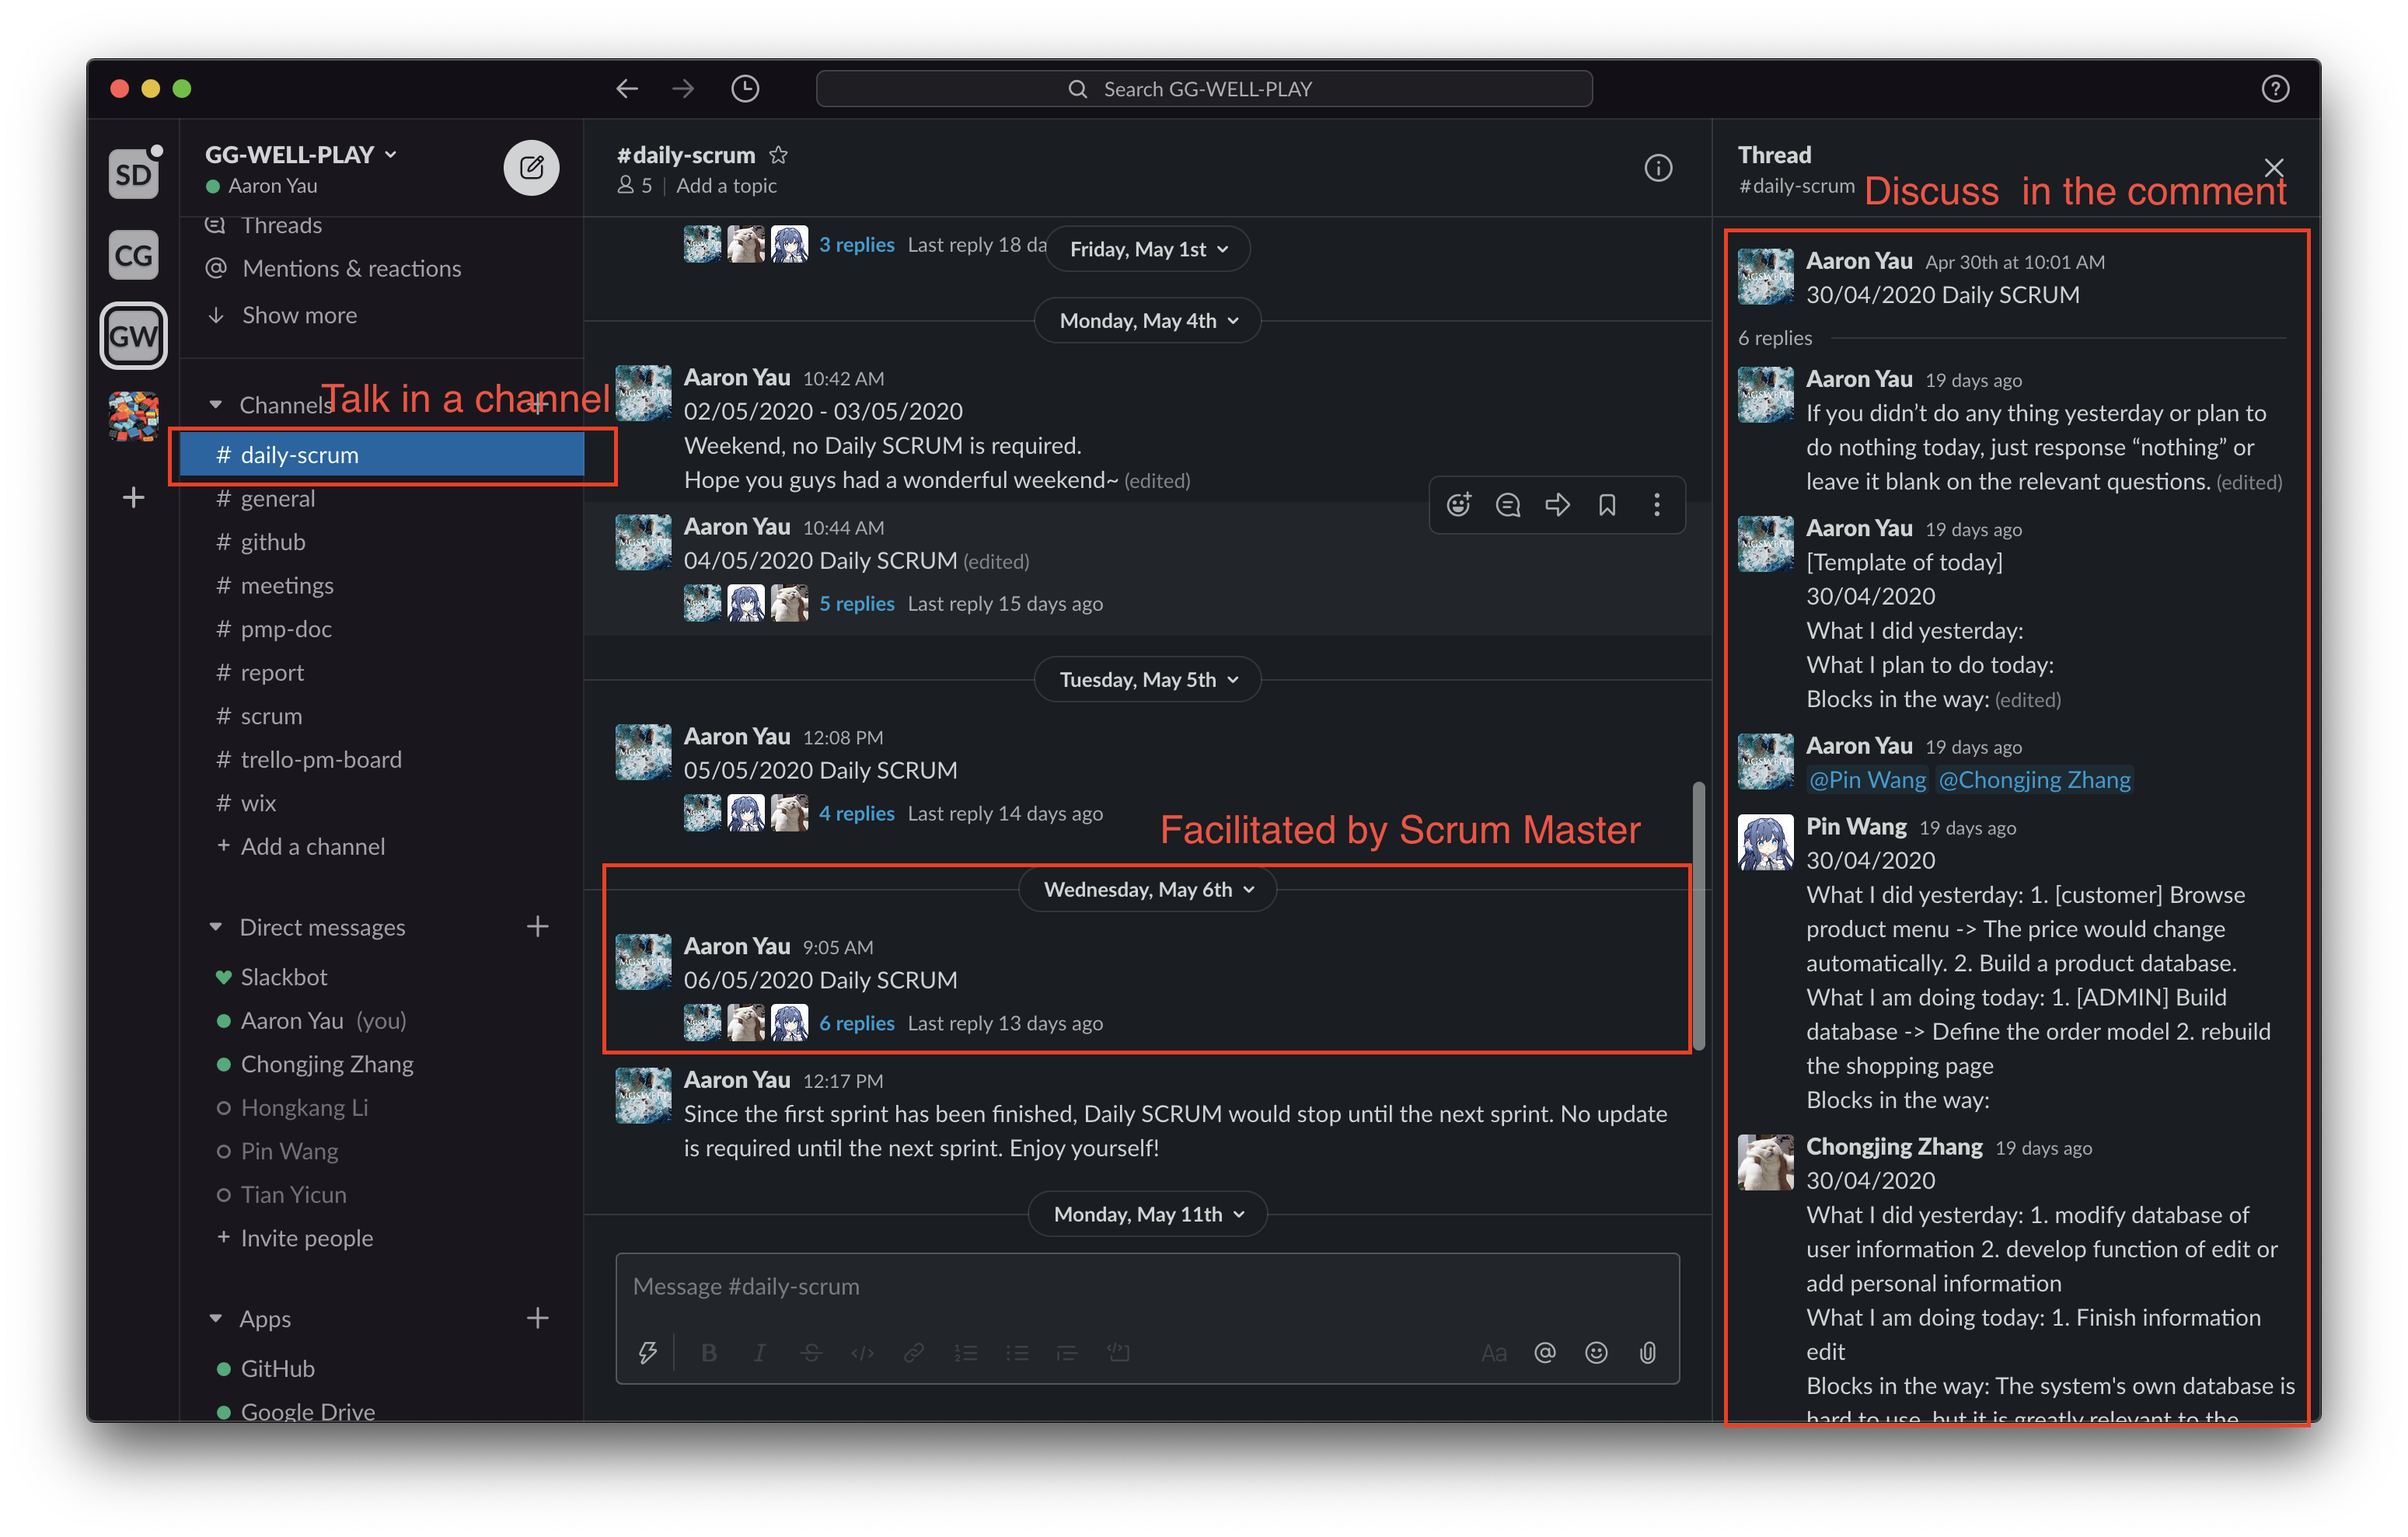
\includegraphics[width=\textwidth]{Figures/dailyScrum.png}
\caption{Daily Scrum Standup Meeting System Example}
\label{fig:dailyScrum}
\end{figure}

\clearpage
\begin{tabularx}{0.95\linewidth}{%
  >{\raggedright\arraybackslash}p{0.2\linewidth}%
  >{\raggedright\arraybackslash}p{0.65\linewidth}}%
  \toprule
  Date & Daily Scrum Standup Meeting Record\\
  \midrule
  April, 27, 2020
  & 
  Zhaofeng Qiu:
  \begin{itemize}
    \item Now, since this is the first day of our first sprint. Only "What I plan to do today" is required.
  \end{itemize}
  Pin Wang:
  \begin{itemize}
    \item What I plan to do today: 
    \begin{enumerate}
      \item Implement feature: [customer] Browse product menu -> Provide a page for showing the list of the products
    \end{enumerate}
  \end{itemize}
  Chongjing Zhang:
  \begin{itemize}
    \item What I plan to do today: 
    \begin{enumerate}
      \item Implement feature: [customer] Sign in -> Provide a page for sign-in
    \end{enumerate}
  \end{itemize}
  %%%%%%%%%%%%%%%%%%%%%%%%%%%%%%%%%%%%%%%%%%%%%%%%%%%%%%%%%%%%%%%%%%%%
  \\
  \midrule
  April, 28, 2020
  & 
  Zhaofeng Qiu:
  \begin{itemize}
    \item Please move the card you are doing to “in progress”.
    \item Send the thing you have to cover in the meeting in format.
  \end{itemize}
  Pin Wang:
  \begin{itemize}
    \item What I did yesterday: 
    \begin{enumerate}
      \item Implement feature: [customer] Browse product menu -> Provide a page for showing the list of the products
    \end{enumerate}
    \item What I plan to do today: 
    \begin{enumerate}
      \item Implement feature: [customer] Browse product menu -> Can see the picture of the products. Can see the price of the products. Can see the types of the products.
    \end{enumerate}
    \item Blocks in the way: 
    \begin{enumerate}
      \item Wix doesn't support its built in check out function unless joining its premium plan. A check out/place order page might need to be implemented manually. 
    \end{enumerate}
  \end{itemize}
  Chongjing Zhang:
  \begin{itemize}
    \item What I did yesterday: 
    \begin{enumerate}
      \item Implement feature: Implement feature:[customer] Sign in -> Provide a page for sign-in
    \end{enumerate}
    \item What I plan to do today:
      \begin{enumerate}
        \item Implement feature: [customer] Sign in and sign out 
        \item Implement feature: [Admin]Sign in and sign out 
        \item Implement feature: [Customer] Sign up  
        \item Create related database
      \end{enumerate}
    \item Blocks in the way: Nothing.
  \end{itemize}
  %%%%%%%%%%%%%%%%%%%%%%%%%%%%%%%%%%%%%%%%%%%%%%%%%%%%%%%%%%%%%%%%%%%%
  \\
  \midrule
  April, 29, 2020
  & 
  Zhaofeng Qiu:
  \begin{itemize}
    \item @Pin Wang @Chongjing Zhang You guys have to figure out the solution of the Wix problem.
  \end{itemize}
  Pin Wang:
  \begin{itemize}
    \item What I did yesterday: 
    \begin{enumerate}
      \item Implement feature: [customer] Browse product menu -> Can see the picture of the products. Can see the price of the products. Can see the types of the products.
    \end{enumerate}
    \item What I plan to do today: 
    \begin{enumerate}
      \item Implement feature: [customer] Browse product menu -> The price would change automatically. 
      \item Implement feature: Build a product database.
    \end{enumerate}
    \item Blocks in the way: 
    \begin{enumerate}
      \item Wix's built in shop doesn't support customize, need to create shopping page, product details page, and place order page manually.
    \end{enumerate}
  \end{itemize}
  Chongjing Zhang:
  \begin{itemize}
    \item What I did yesterday: 
    \begin{enumerate}
      \item Implement feature: [customer] Sign in and sign out 
      \item Implement feature: [Admin]Sign in and sign out 
      \item Implement feature: [Customer] Sign up  
      \item Create related database
    \end{enumerate}
    \item What I plan to do today: 
    \begin{enumerate}
      \item Implement feature: modify database of user information 
      \item Implement feature: develop function of edit or add personal information
    \end{enumerate}
    \item Blocks in the way: 
    \begin{enumerate}
      \item Some function can't change in Wix model, so maybe it needs to modify or even redo.
    \end{enumerate}
  \end{itemize}
  \\
  %%%%%%%%%%%%%%%%%%%%%%%%%%%%%%%%%%%%%%%%%%%%%%%%%%%%%%%%%%%%%%%%%%%%
  \\
  \midrule
  April, 30, 2020
  & 
  Zhaofeng Qiu:
  \begin{itemize}
    \item @Pin Wang @Chongjing Zhang If you didn’t do any thing yesterday or plan to do nothing today, just response “nothing” or leave it blank on the relevant questions. 
    \item I will tell Yicun about the problem of database.
  \end{itemize}
  Pin Wang:
  \begin{itemize}
    \item What I did yesterday: 
    \begin{enumerate}
      \item Implement feature: [customer] Browse product menu -> The price would change automatically.  
      \item Build a product database.
    \end{enumerate}
    \item What I plan to do today: 
    \begin{enumerate}
      \item Implement feature: [ADMIN] Build database -> Define the order model
      \item rebuild the shopping page
    \end{enumerate}
    \item Blocks in the way: 
    \begin{enumerate}
      \item Nothing.
    \end{enumerate}
  \end{itemize}
  Chongjing Zhang:
  \begin{itemize}
    \item What I did yesterday: 
    \begin{enumerate}
      \item Modify database of user information  
      \item Develop function of edit or add personal information
    \end{enumerate}
    \item What I plan to do today: 
    \begin{enumerate}
      \item Finish information edit.
    \end{enumerate}
    \item Blocks in the way: 
    \begin{enumerate}
      \item The system's own database is hard to use, but it is greatly relevant to the entire model. I'm trying to find some methods to code in the backend to acquire data in db.
    \end{enumerate}
  \end{itemize}
  \\
  %%%%%%%%%%%%%%%%%%%%%%%%%%%%%%%%%%%%%%%%%%%%%%%%%%%%%%%%%%%%%%%%%%%%
  \\
  \midrule
  May, 01, 2020
  & 
  Zhaofeng Qiu:
  \begin{itemize}
    \item Daily SCRUM time! 
    \item Why you don't want to do any thing today? @Chongjing Zhang
  \end{itemize}
  Pin Wang:
  \begin{itemize}
    \item What I did yesterday: 
    \begin{enumerate}
      \item Implement feature: [ADMIN] Build database -> Define the order model
    \end{enumerate}
    \item What I plan to do today: 
    \begin{enumerate}
      \item rebuild the shopping page
    \end{enumerate}
    \item Blocks in the way: 
    \begin{enumerate}
      \item Nothing.
    \end{enumerate}
  \end{itemize}
  Chongjing Zhang:
  \begin{itemize}
    \item Reply to Scrum Master:
    \begin{enumerate}
      \item Because my part is based on Pin Wang's part, which isn't finished.
    \end{enumerate}
    \item What I did yesterday: 
    \begin{enumerate}
      \item Finish information edit 
      \item Improve database functions and code in backend
    \end{enumerate}
    \item What I plan to do today:
      \begin{enumerate}
        \item Nothing.
      \end{enumerate}
    \item Blocks in the way: 
      \begin{enumerate}
        \item My part is based on Pin Wang's part, which isn't finished.
      \end{enumerate}
  \end{itemize}
  \\
  %%%%%%%%%%%%%%%%%%%%%%%%%%%%%%%%%%%%%%%%%%%%%%%%%%%%%%%%%%%%%%%%%%%%
  \\
  \midrule
  May, 02, 2020 - May, 03, 2020
  & Weekend, no Daily Scrum
  %%%%%%%%%%%%%%%%%%%%%%%%%%%%%%%%%%%%%%%%%%%%%%%%%%%%%%%%%%%%%%%%%%%%
  \\
  \midrule
  May, 04, 2020
  & 
  Zhaofeng Qiu:
  \begin{itemize}
    \item Hope you guys had a wonderful weekend.
  \end{itemize}
  Pin Wang:
  \begin{itemize}
    \item What I did last Friday: 
    \begin{enumerate}
      \item Rebuild the shopping page and product details page 
    \end{enumerate}
    \item What I plan to do today: 
    \begin{enumerate}
      \item Implement feature: [Admin] Manage product infomation-> 1. Add product 2. Delete product
    \end{enumerate}
    \item Blocks in the way: 
    \begin{enumerate}
      \item 
    \end{enumerate}
  \end{itemize}
  Chongjing Zhang:
  \begin{itemize}
    \item What I did last Friday: 
    \begin{enumerate}
      \item Nothing.
    \end{enumerate}
    \item What I plan to do today:
      \begin{enumerate}
        \item Modify database 
        \item Fix problem of connecting system own's database and created database
      \end{enumerate}
    \item Blocks in the way: 
      \begin{enumerate}
        \item Nothing.
      \end{enumerate}
  \end{itemize}
  \\
  %%%%%%%%%%%%%%%%%%%%%%%%%%%%%%%%%%%%%%%%%%%%%%%%%%%%%%%%%%%%%%%%%%%%
  \\
  \midrule
  May, 05, 2020
  & 
  Zhaofeng Qiu:
  \begin{itemize}
    \item @Pin Wang @Chongjing Zhang 
  \end{itemize}
  Pin Wang:
  \begin{itemize}
    \item What I did yesterday: 
    \begin{enumerate}
      \item Implement feature: [Admin] Manage product infomation-> 1. Add product 2. Delete product
    \end{enumerate}
    \item What I plan to do today: 
    \begin{enumerate}
      \item Implement feature: [Admin] Manage product infomation-> 1. Change the price of products 2. Change the pictures of products 3. Change the type of products
    \end{enumerate}
    \item Blocks in the way: 
    \begin{enumerate}
      \item 
    \end{enumerate}
  \end{itemize}
  Chongjing Zhang:
  \begin{itemize}
    \item What I did yesterday: 
    \begin{enumerate}
      \item Modify database 
      \item Fix problem of connecting system own's database and created database
    \end{enumerate}
    \item What I plan to do today:
      \begin{enumerate}
        \item Nothing.
      \end{enumerate}
    \item Blocks in the way: 
      \begin{enumerate}
        \item Nothing.
      \end{enumerate}
  \end{itemize}
  \\
  %%%%%%%%%%%%%%%%%%%%%%%%%%%%%%%%%%%%%%%%%%%%%%%%%%%%%%%%%%%%%%%%%%%%
  \\
  \midrule
  May, 06, 2020
  & 
  Zhaofeng Qiu:
  \begin{itemize}
    \item @Pin Wang @Chongjing Zhang Is everything going well? It seems that the database feature has been in “in Progress” for many days. If there is any problem, tell me in “Blocks in the way”.
  \end{itemize}
  Pin Wang:
  \begin{itemize}
    \item What I did yesterday: 
    \begin{enumerate}
      \item [Admin] Manage product infomation-> 1. Change the price of products 2. Change the pictures of products 3. Change the type of products.
    \end{enumerate}
    \item What I plan to do today: 
    \begin{enumerate}
      \item Test functions of website, make sure everything go well
    \end{enumerate}
    \item Blocks in the way: 
    \begin{enumerate}
      \item Nothing.
    \end{enumerate}
  \end{itemize}
  Chongjing Zhang:
  \begin{itemize}
    \item Reply to Scrum Master:
    \begin{enumerate}
      \item Sorry, we've finished yet, just forget to move it to done.
    \end{enumerate}
    \item What I did yesterday: 
    \begin{enumerate}
      \item Implement feature: 
    \end{enumerate}
    \item What I plan to do today:
      \begin{enumerate}
        \item Test functions of website, make sure everything go well
      \end{enumerate}
    \item Blocks in the way: 
      \begin{enumerate}
        \item Nothing.
      \end{enumerate}
  \end{itemize}
  \\
  %%%%%%%%%%%%%%%%%%%%%%%%%%%%%%%%%%%%%%%%%%%%%%%%%%%%%%%%%%%%%%%%%%%%
  \\
  \midrule
  May, 07, 2020 - May, 10, 2020
  & Zhaofeng Qiu:
  \begin{itemize}
    \item Since the features in the first sprint has been finished, Daily SCRUM would stop until the next sprint. No update is required until the next sprint. Enjoy yourself!
  \end{itemize}
  %%%%%%%%%%%%%%%%%%%%%%%%%%%%%%%%%%%%%%%%%%%%%%%%%%%%%%%%%%%%%%%%%%%%
  \\
  \midrule
  May, 11, 2020
  &
  Zhaofeng Qiu:
  \begin{itemize}
    \item  Daily SCRUM @Pin Wang @Chongjing Zhan. From now on, the Daily Scrum would only be held on Monday, Wednesday and Friday.
  \end{itemize}

  Pin Wang:
  \begin{itemize}
    \item What I plan to do today \& tomorrow: 
    \begin{enumerate}
      \item Build cart database.  
      \item Implement feature: [customer] Add products to shopping cart. 3. [customer] Check out shopping cart -> (1) Show the day and time which is valid (2) Choose a day and time for delivery.
    \end{enumerate}
    \item Blocks in the way: 
    \begin{enumerate}
      \item Nothing.
    \end{enumerate}
  \end{itemize}

  Chongjing Zhang:
  \begin{itemize}
    \item What I plan to do today \& tomorrow:
    \begin{enumerate}
      \item Build cart and order database. 
      \item Link cart database with user information and develop functions of add and delete items in the cart. 
      \item Implement functions of select items to pay. 
      \item Implement functions of change items size or/and quantity in cart. 
      \item Implement functions of viewing total prices in cart. 
      \item Implement functions of showing all items.
    \end{enumerate}
    \item Blocks in the way: 
    \begin{enumerate}
      \item Unfamiliar with wix query method - "then", spend much time in debugging.
    \end{enumerate}
  \end{itemize}
  %%%%%%%%%%%%%%%%%%%%%%%%%%%%%%%%%%%%%%%%%%%%%%%%%%%%%%%%%%%%%%%%%%%%
  \\
  \midrule
  May, 12, 2020
  & No Daily Scrum on Tuesday in the second sprint. Canceled based on dicision in the first sprint retrospective.
  %%%%%%%%%%%%%%%%%%%%%%%%%%%%%%%%%%%%%%%%%%%%%%%%%%%%%%%%%%%%%%%%%%%%
  \\
  \midrule
  May, 13, 2020
  & 
  Zhaofeng Qiu:
  \begin{itemize}
    \item @Pin Wang @Chongjing Zhan
  \end{itemize}
  Pin Wang:
  \begin{itemize}
    \item What I did in the last two days: 
    \begin{enumerate}
      \item Build cart database. 
      \item Inplement feature: [customer] Add products to shopping cart. 
      \item Inplement feature: [customer] Check out shopping cart -> (1) Show the day and time which is valid (2) Choose a day and time for delivery.
    \end{enumerate}
    \item What I plan to do today \& tomorrow: 
    \begin{enumerate}
      \item Inplement feature: [customer] Check out shopping cart -> (1) Handle synchronization problem (2) Get a confirming email. (3) Add an order to the user's order list.
    \end{enumerate}
    \item Blocks in the way: 
    \begin{enumerate}
      \item Nothing.
    \end{enumerate}
  \end{itemize}
  Chongjing Zhang:
  \begin{itemize}
    \item What I did in the last two days: 
    \begin{enumerate}
      \item Build cart and order database. 
      \item Link cart database with user information and develop functions of add and delete items in the cart. 
      \item Implement functions of select items to pay. 
      \item Implement functions of change items size or/and quantity in cart. 
      \item Implement functions of viewing total prices in cart. 
      \item Implement functions of showing all items.  
    \end{enumerate}
    \item What I plan to do today \& tomorrow:
      \begin{enumerate}
        \item Implement feature: 
      \end{enumerate}
    \item Blocks in the way: 
      \begin{enumerate}
        \item We want to nest a repeater inside a repeater, but it seems impossible to implement in wix, so we need to find out other methods to solve this problem.
      \end{enumerate}
  \end{itemize}
  %%%%%%%%%%%%%%%%%%%%%%%%%%%%%%%%%%%%%%%%%%%%%%%%%%%%%%%%%%%%%%%%%%%%
  \\
  \midrule
  May, 14, 2020
  & No Daily Scrum on Tuesday in the second sprint. Canceled based on dicision in the first sprint retrospective.
  %%%%%%%%%%%%%%%%%%%%%%%%%%%%%%%%%%%%%%%%%%%%%%%%%%%%%%%%%%%%%%%%%%%%
  \\
  \midrule
  May, 15, 2020 
  & 
  Zhaofeng Qiu:
  \begin{itemize}
    \item @Pin Wang @Chongjing Zhan Daily SCRUM
    \item It seems the risk of Wix happend.
  \end{itemize}
  Pin Wang:
  \begin{itemize}
    \item What I did in the last two days: 
    \begin{enumerate}
      \item Implement feature: [customer] Check out shopping cart -> (1) Handle synchronization problem (3) Add an order to the user's order list. Partialy done (2): send a confirmation email
    \end{enumerate}
    \item What I plan to do today: 
    \begin{enumerate}
      \item Finish send confirmation email. 
      \item Implement feature: [Customer] Cancel orders
    \end{enumerate}
    \item Blocks in the way: 
    \begin{enumerate}
      \item The email template offered by Wix isn't very helpful for showing all order details. Need to find a alternative way to complete this function.
    \end{enumerate}
  \end{itemize}
  Chongjing Zhang:
  \begin{itemize}
    \item What I did in the last two days: 
    \begin{enumerate}
      \item Rebuild userinfo database 
      \item Rebuild user address page 
      \item Add confirmation to delete in cart page. 
      \item Sum money to items only selected. 
      \item Modify some UI and design in interfaces. 
      \item Edit order database. 
      \item Design order page 
    \end{enumerate}
    \item What I plan to do today \& tomorrow:
      \begin{enumerate}
        \item Implement feature: [Customer]Design order page 2. Connect this page to database so that all orders could be shown correctly 3. [Admin] Design order management page
      \end{enumerate}
    \item Blocks in the way: 
      \begin{enumerate}
        \item Wix doesn't support nest a repeater inside a repeater, so need to find a way to make a beautiful page
      \end{enumerate}
  \end{itemize}
  %%%%%%%%%%%%%%%%%%%%%%%%%%%%%%%%%%%%%%%%%%%%%%%%%%%%%%%%%%%%%%%%%%%%
  \\
  \midrule
  May, 16, 2020 -  May, 17, 2020
  & Weekend, no Daily Scrum
  %%%%%%%%%%%%%%%%%%%%%%%%%%%%%%%%%%%%%%%%%%%%%%%%%%%%%%%%%%%%%%%%%%%%
  \\
  \midrule
  May, 18, 2020
  & 
  Zhaofeng Qiu:
  \begin{itemize}
    \item @Pin Wang @Chongjing Zhan Daily SCRUM
  \end{itemize}
  Pin Wang:
  \begin{itemize}
    \item What I did in the last two days: 
    \begin{enumerate}
      \item Implement feature: [customer] Check out shopping cart -> send a confirmation eamil 
    \end{enumerate}
    \item What I plan to do today: 
    \begin{enumerate}
      \item Implement feature: [customer] view and cancel order
    \end{enumerate}
    \item Blocks in the way: 
    \begin{enumerate}
      \item Nothing.
    \end{enumerate}
  \end{itemize}
  Chongjing Zhang:
  \begin{itemize}
    \item What I did in the last two days: 
    \begin{enumerate}
      \item Design UI of order page.
    \end{enumerate}
    \item What I plan to do today \& tomorrow:
      \begin{enumerate}
        \item Implement feature: [admin]finish order management page, improve some functions and finish all rest of work.
      \end{enumerate}
    \item Blocks in the way: 
      \begin{enumerate}
        \item Nothing.
      \end{enumerate}
  \end{itemize}
  \\
  %%%%%%%%%%%%%%%%%%%%%%%%%%%%%%%%%%%%%%%%%%%%%%%%%%%%%%%%%%%%%%%%%%%%
  \\
  \midrule
  May, 19, 2020
  & No Daily Scrum on Tuesday in the second sprint. Canceled based on dicision in the first sprint retrospective.
  %%%%%%%%%%%%%%%%%%%%%%%%%%%%%%%%%%%%%%%%%%%%%%%%%%%%%%%%%%%%%%%%%%%%
  \\
  \midrule
  May, 20, 2020
  & 
  Zhaofeng Qiu:
  \begin{itemize}
    \item @Pin Wang @Chongjing Zhan Daily SCRUM
    \item It seems that all the features in the second sprint have been finish! Good Jobs!
  \end{itemize}
  Pin Wang:
  \begin{itemize}
    \item What I did in the last two days: 
    \begin{enumerate}
      \item Implement feature: [customer] view and cancel order 
    \end{enumerate}
  \end{itemize}
  Chongjing Zhang:
  \begin{itemize}
    \item What I did in the last two days: 
    \begin{enumerate}
      \item Implement feature: [admin] finish order management page, improve some functions and finish all rest of work.
    \end{enumerate}
  \end{itemize}
  \\
  \bottomrule
  \\
  \caption{Daily Scrum Standup Meeting Record}  
  \label{tab:dailyScrumStandupMeetingRecord}
\end{tabularx}  

\chapter*{Appendix C: Product Design}
\addcontentsline{toc}{chapter}{Appendix C: Product Design}

\textbf{Product Menu}
\begin{figure}[htp]
\centering
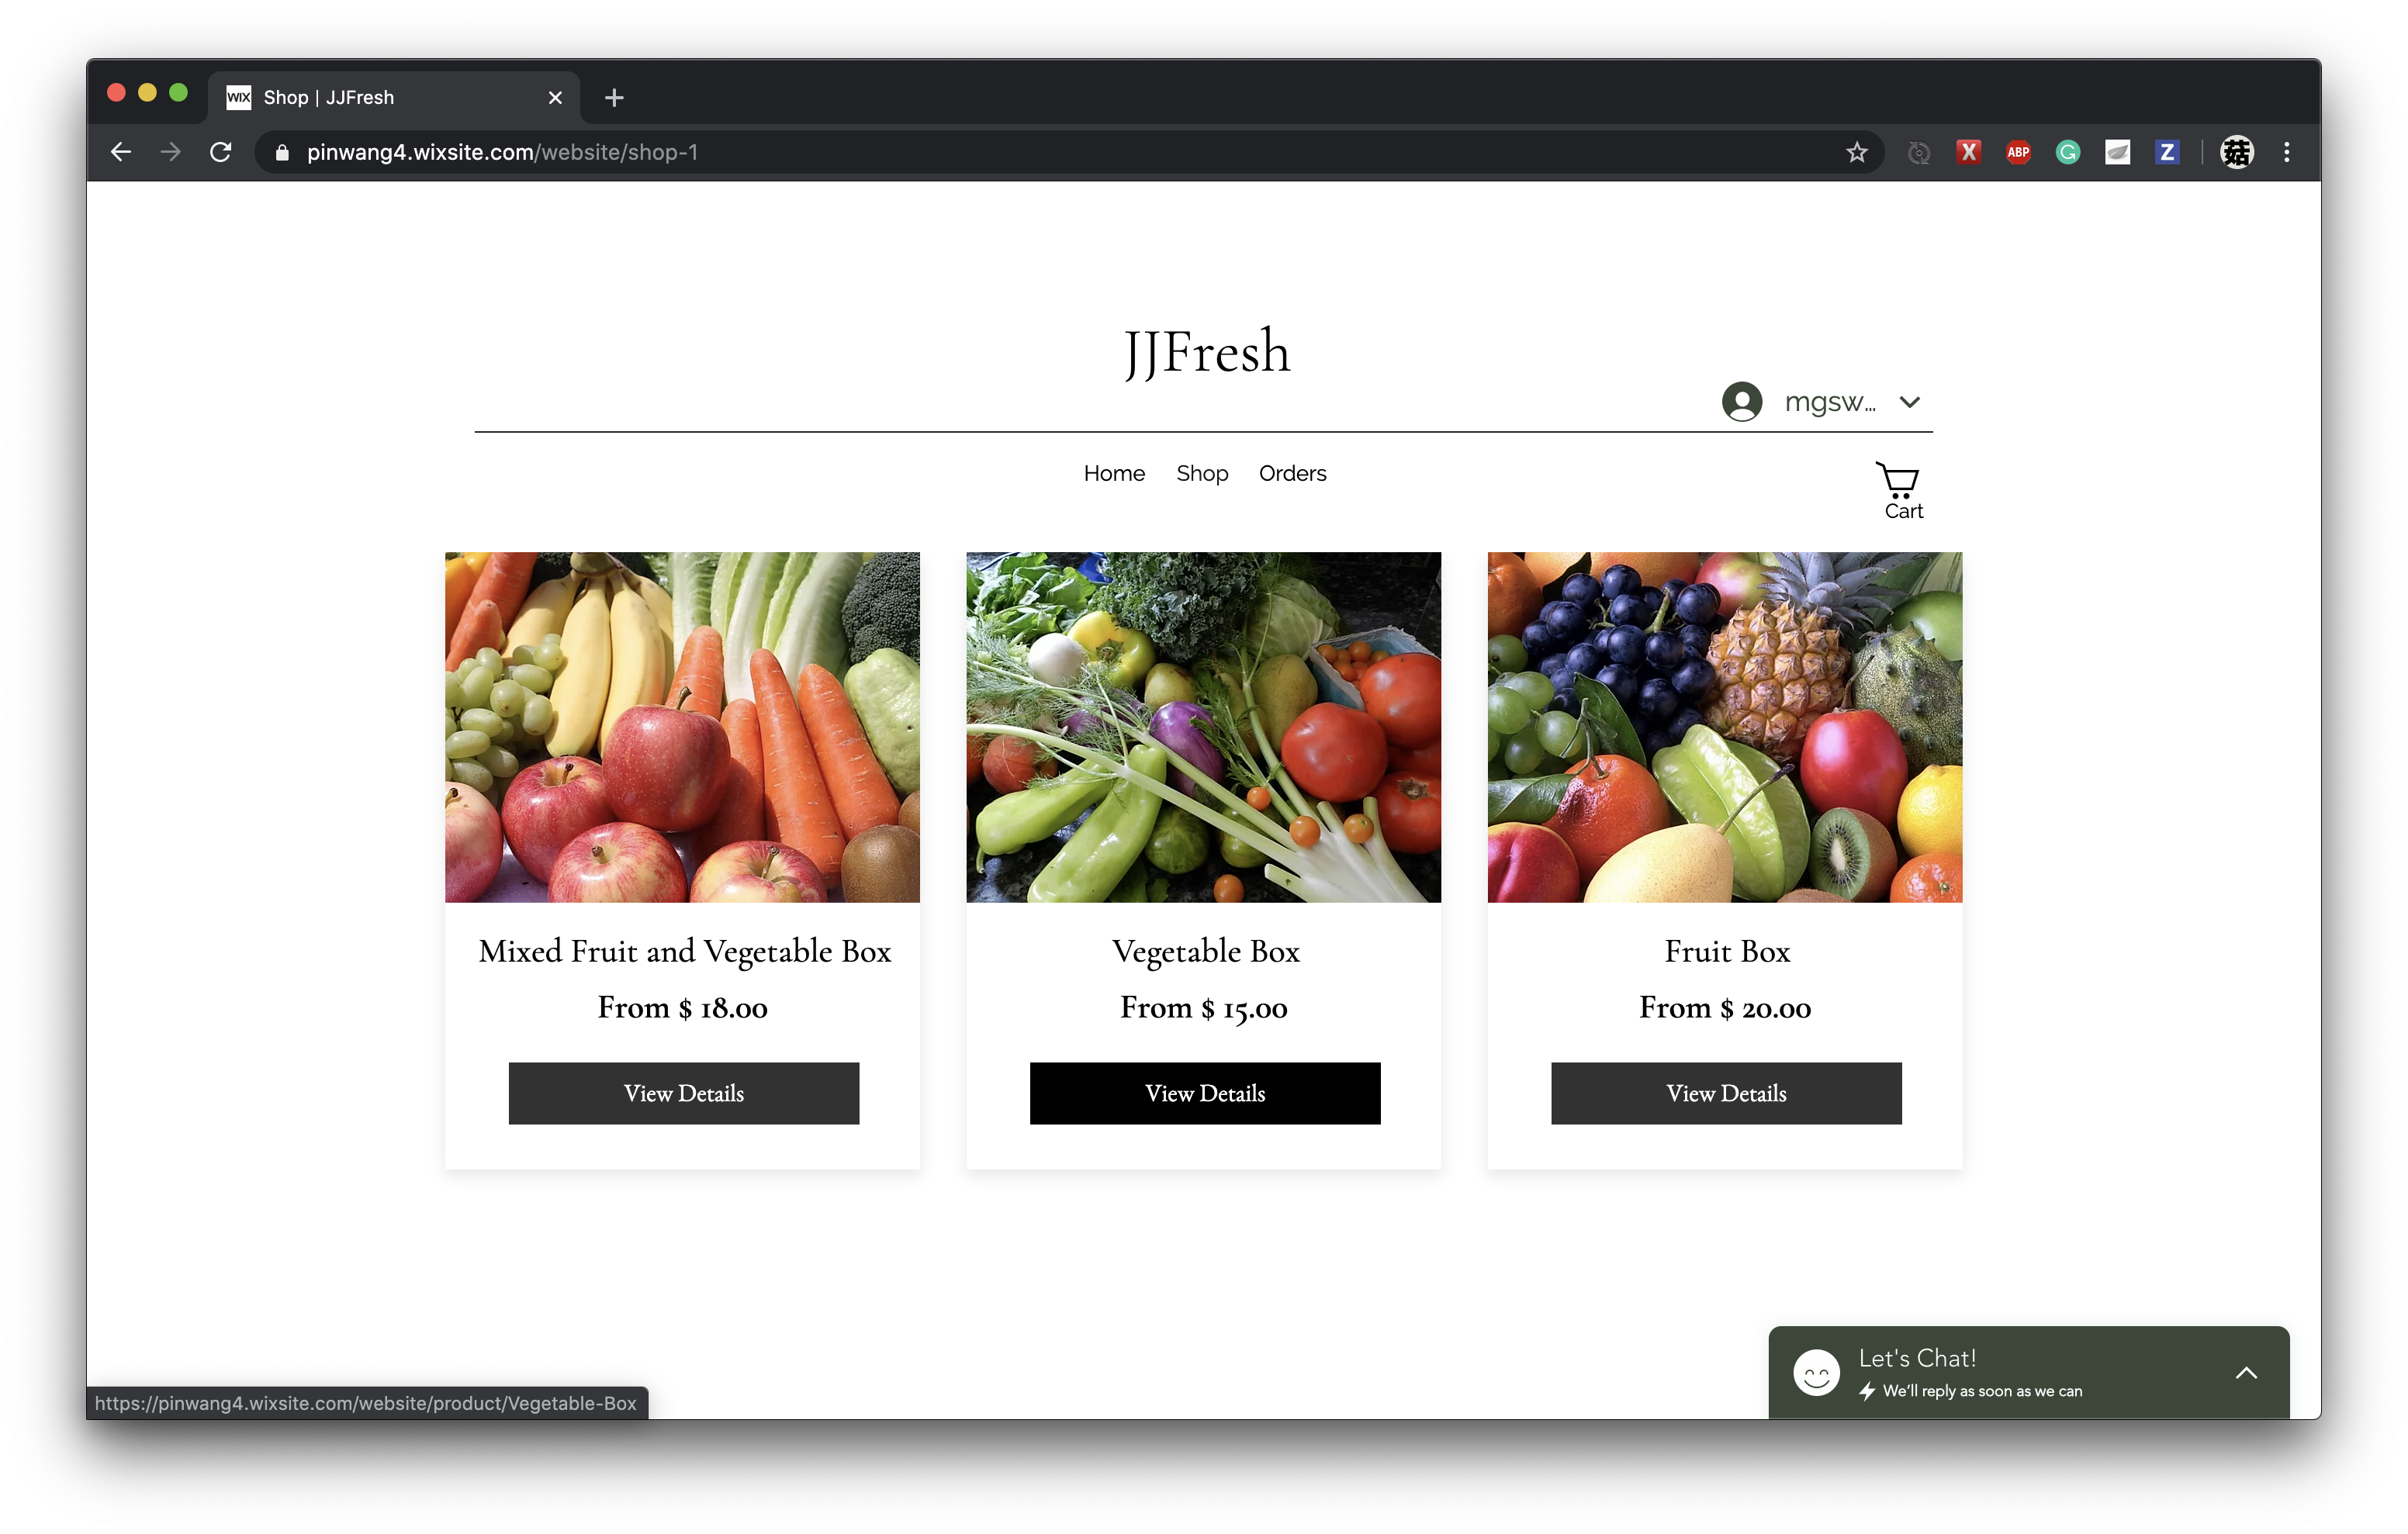
\includegraphics[width=\textwidth]{Figures/productMenu.png}
\caption{Screenshot of Product Menu }
\label{fig:productMenu}
\end{figure}

\clearpage
\textbf{To add product}
\begin{figure}[htp]
\centering
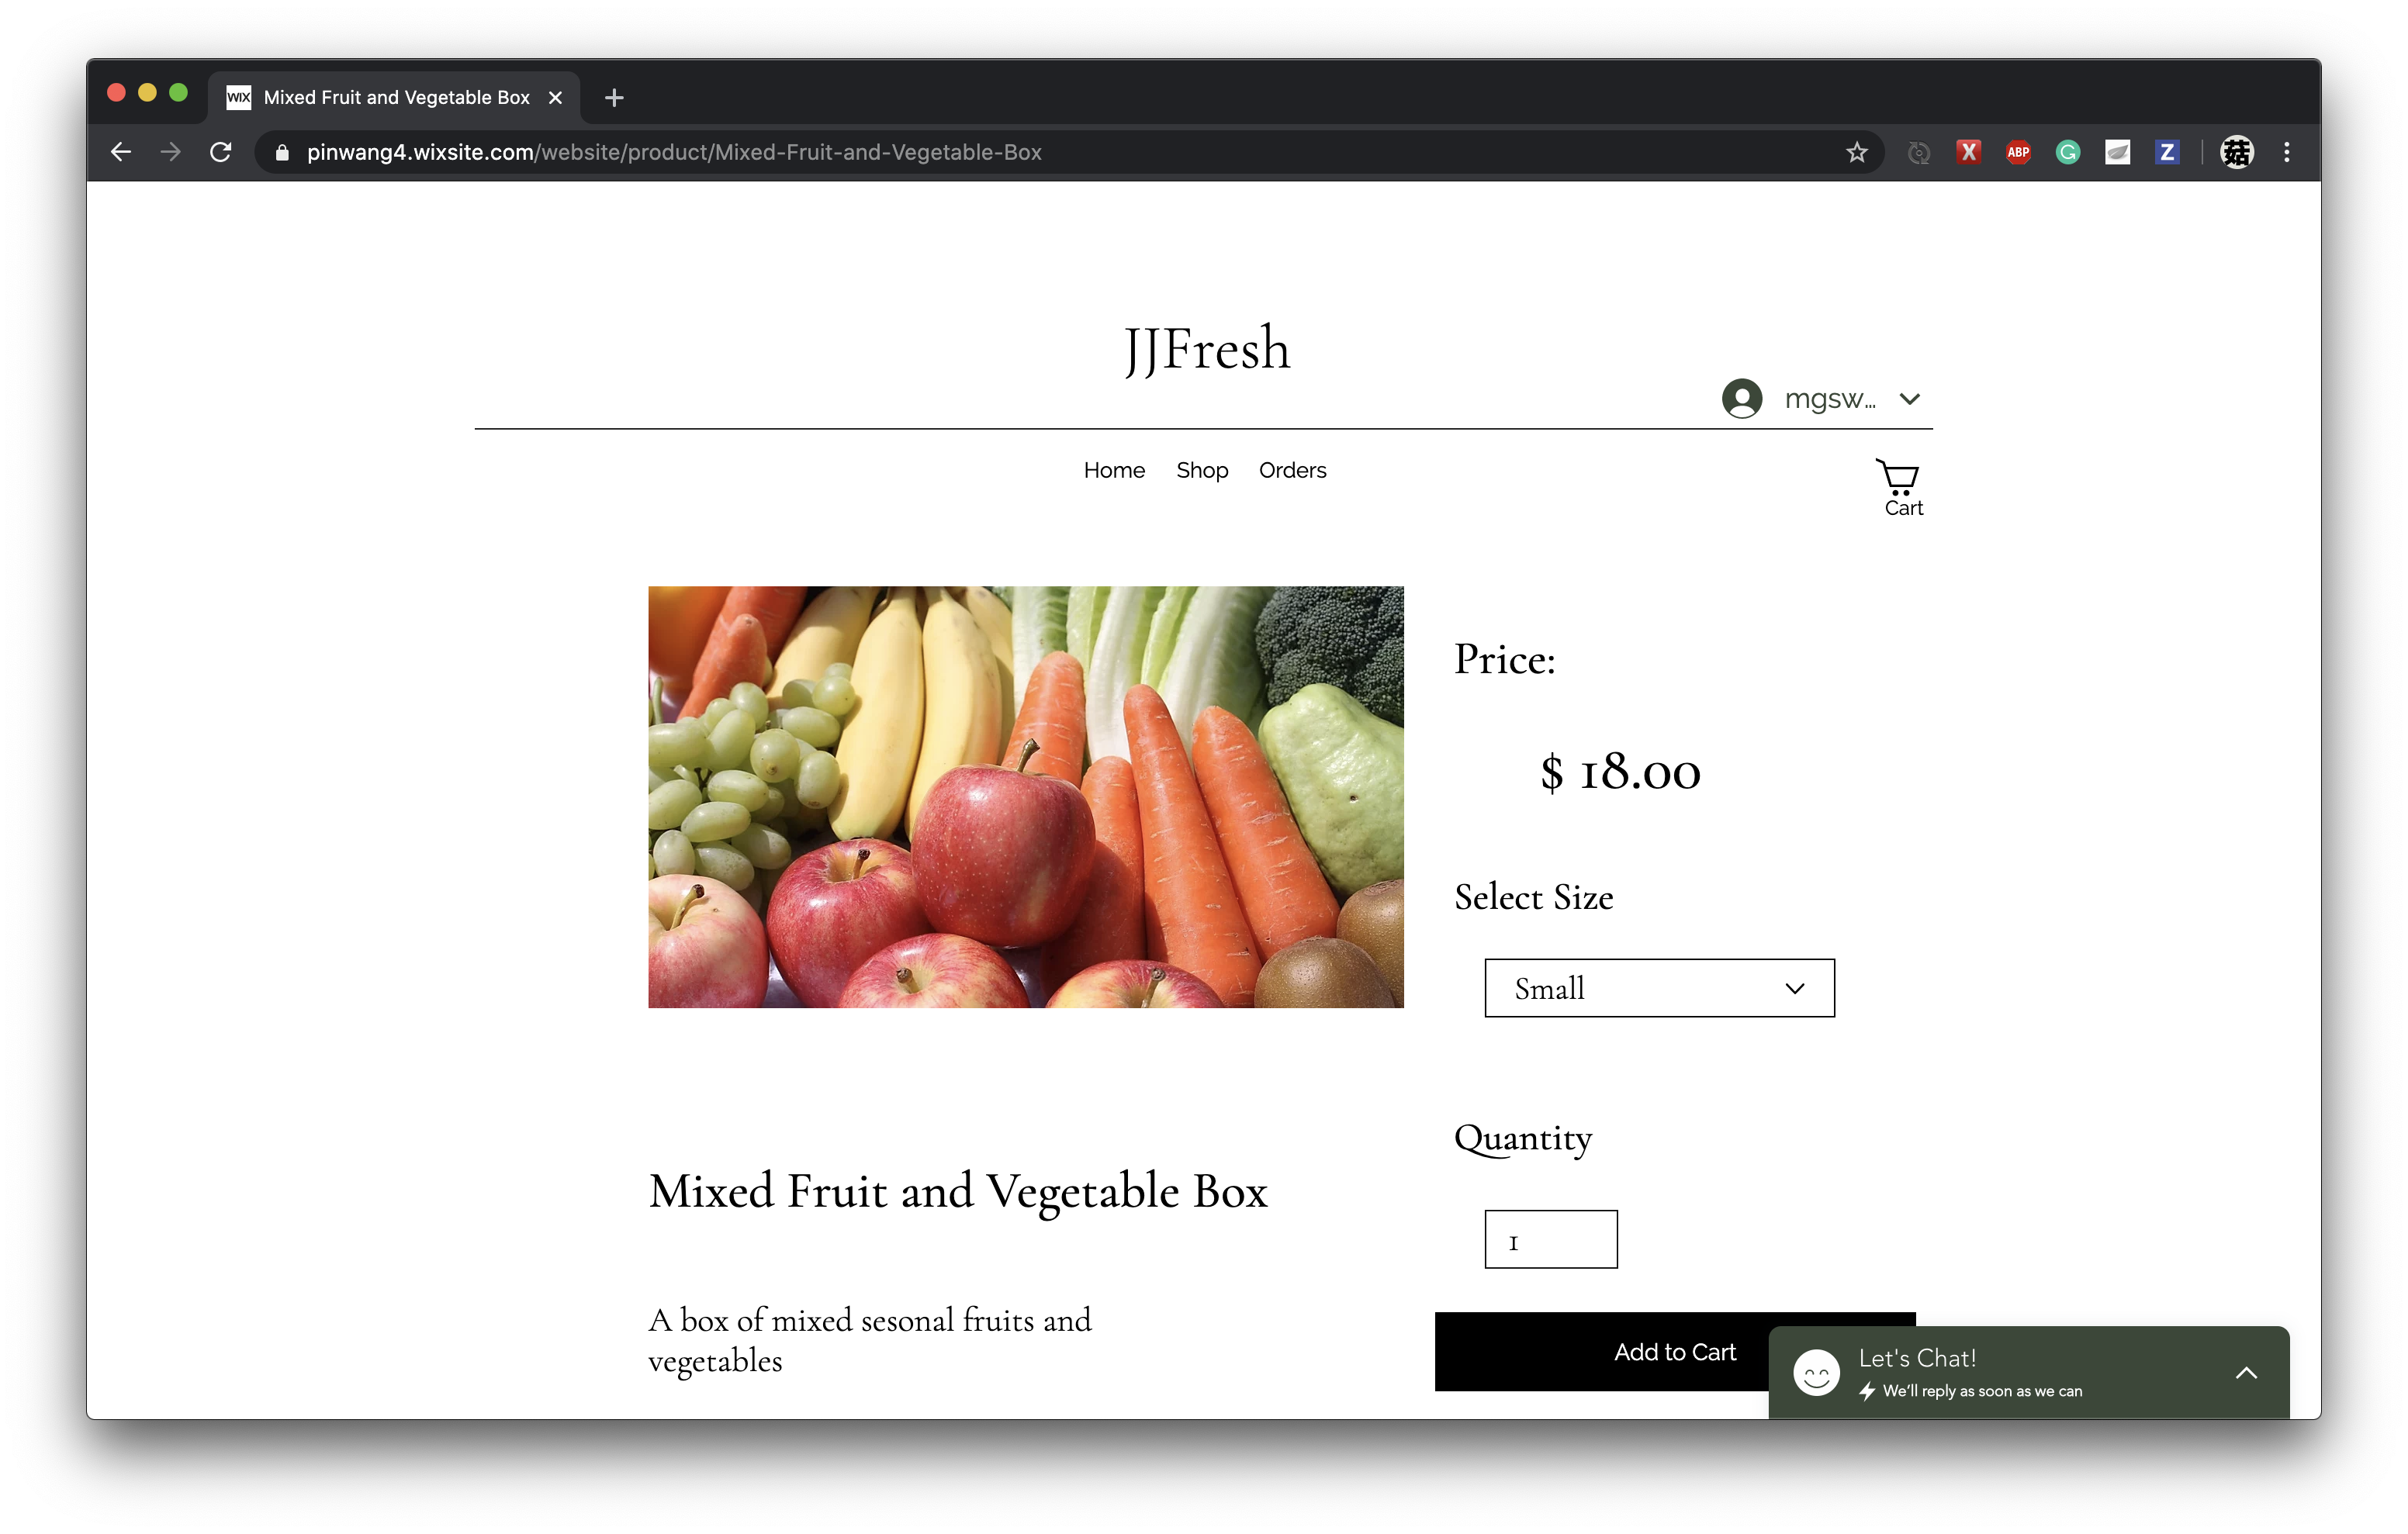
\includegraphics[width=\textwidth]{Figures/addProduct.png}
\caption{Screenshot of adding product}
\label{fig:addProduct}
\end{figure}

\clearpage
\textbf{Shoping cart}
\begin{figure}[htp]
\centering
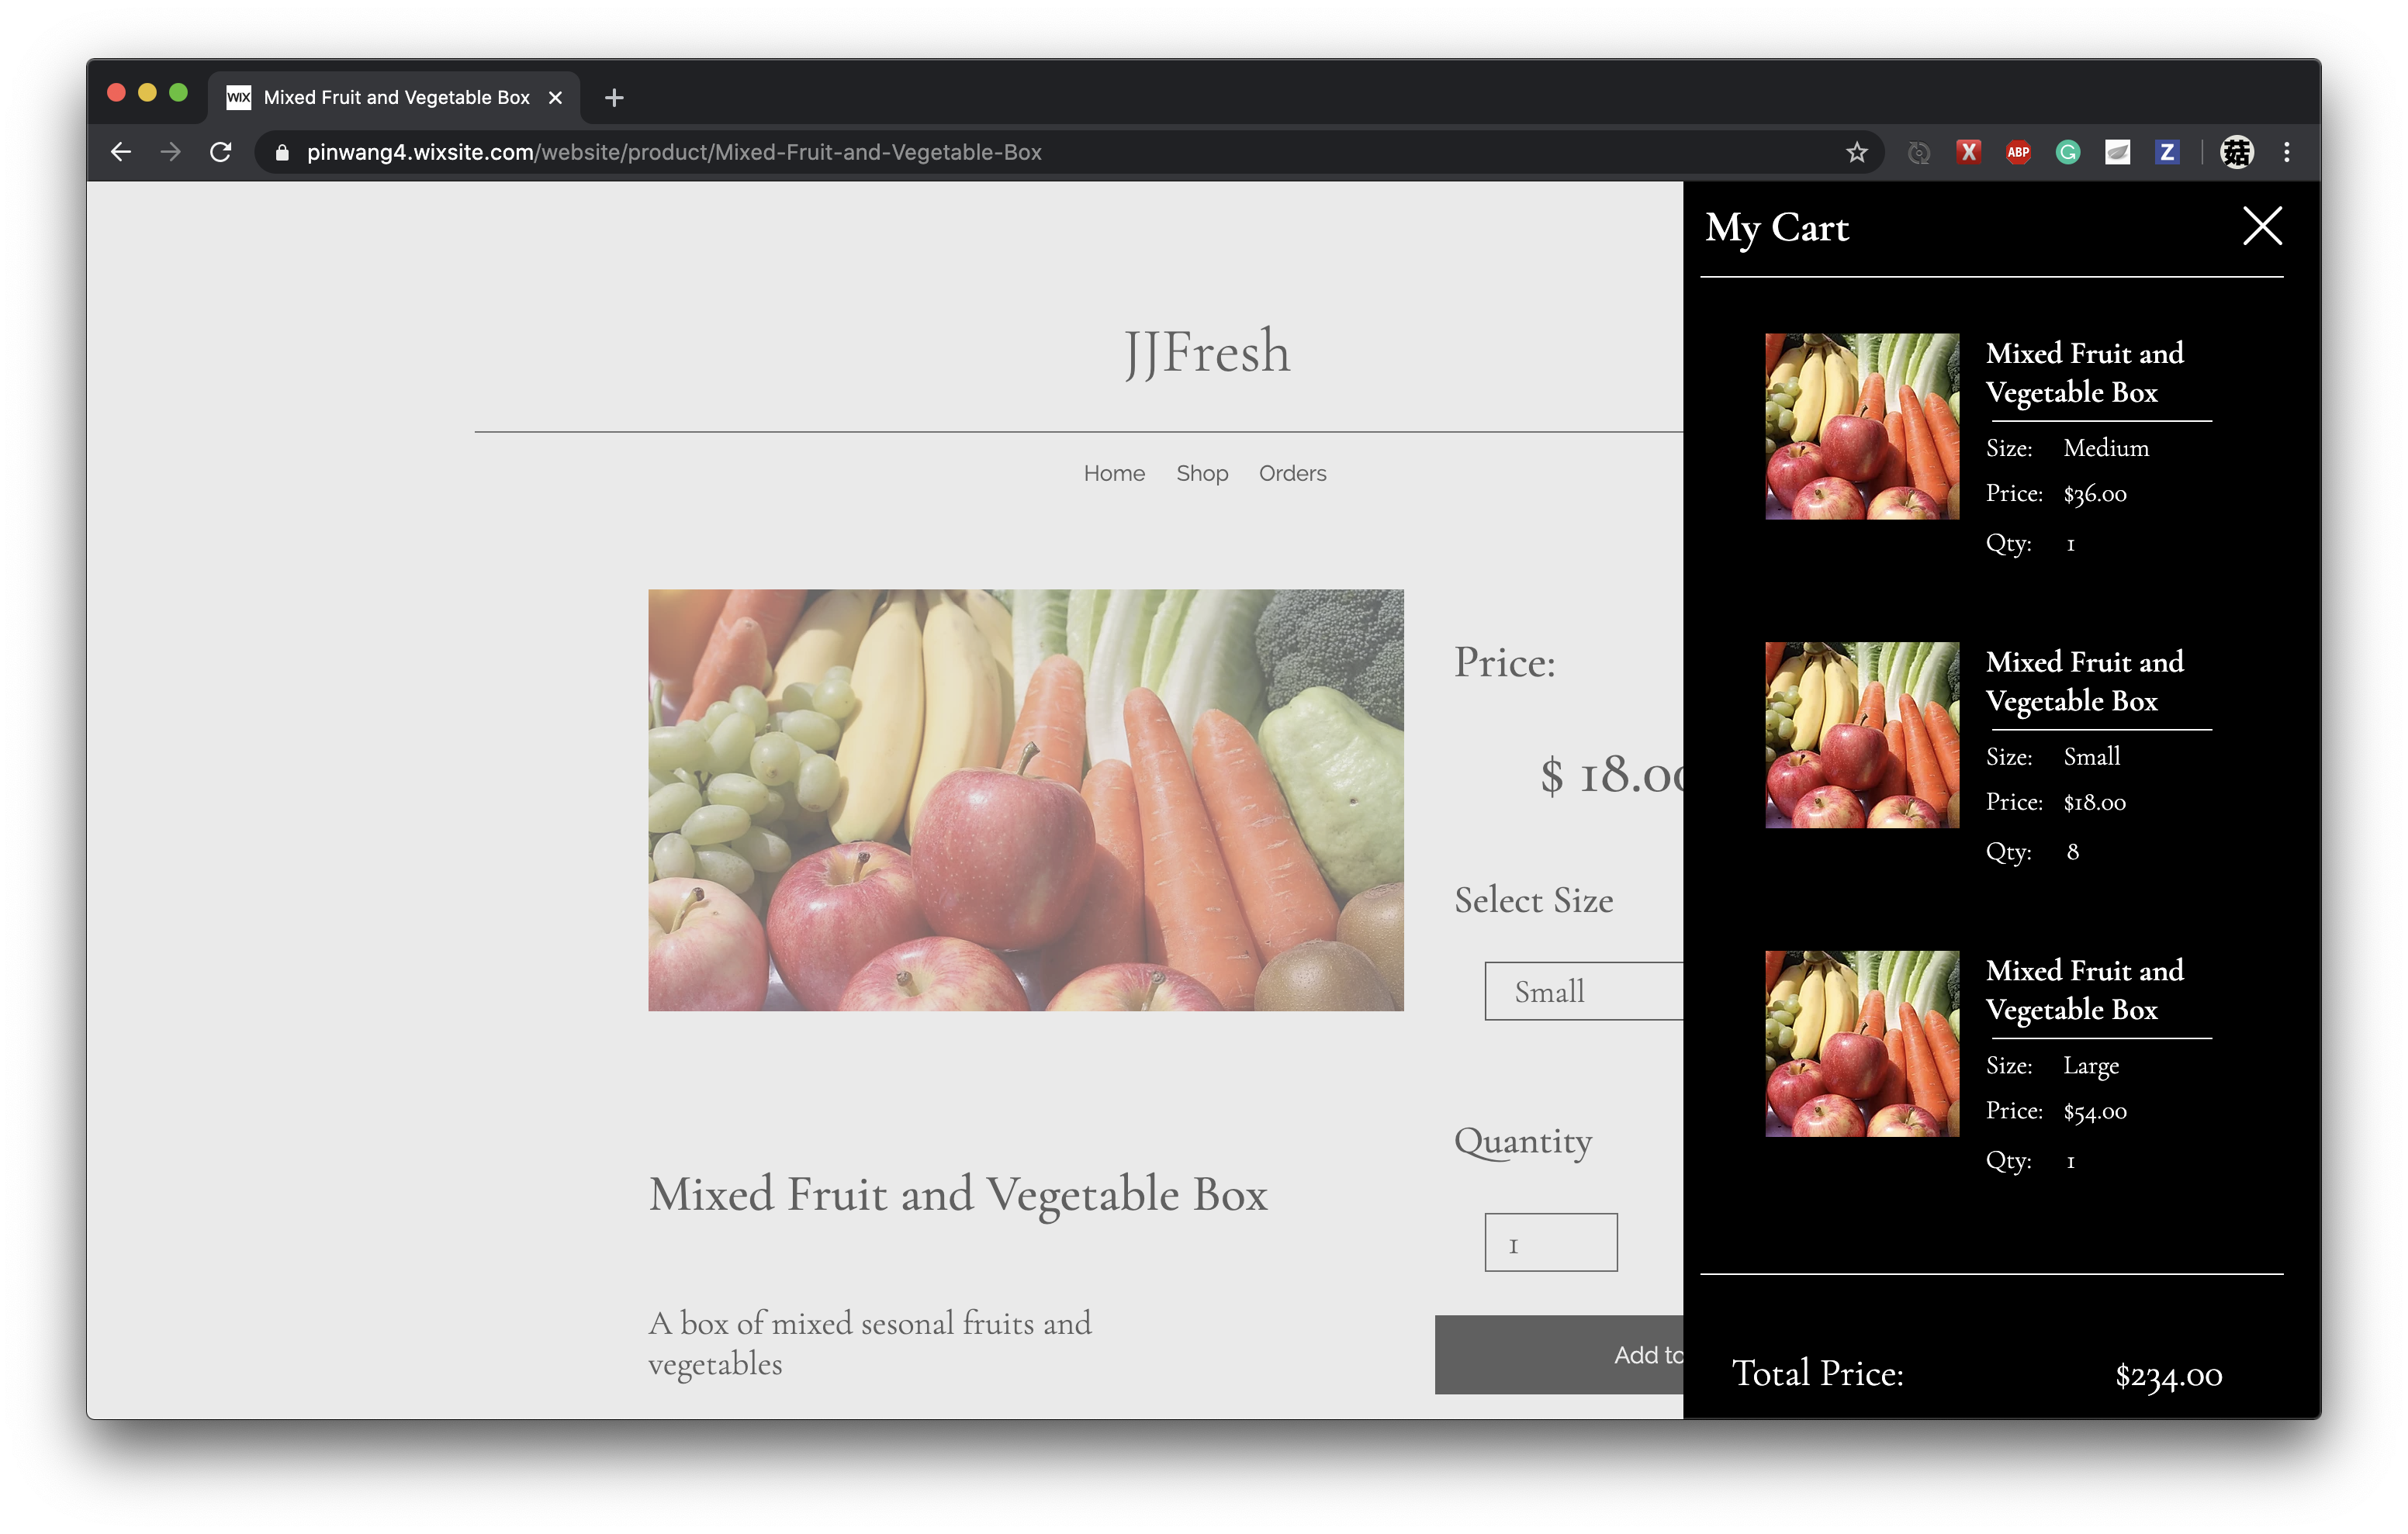
\includegraphics[width=\textwidth]{Figures/shoppingCart.png}
\caption{Screenshot of Shopping Cart}
\label{fig:shoppingCart}
\end{figure}

\clearpage
\textbf{Check out page}
\begin{figure}[htp]
\centering
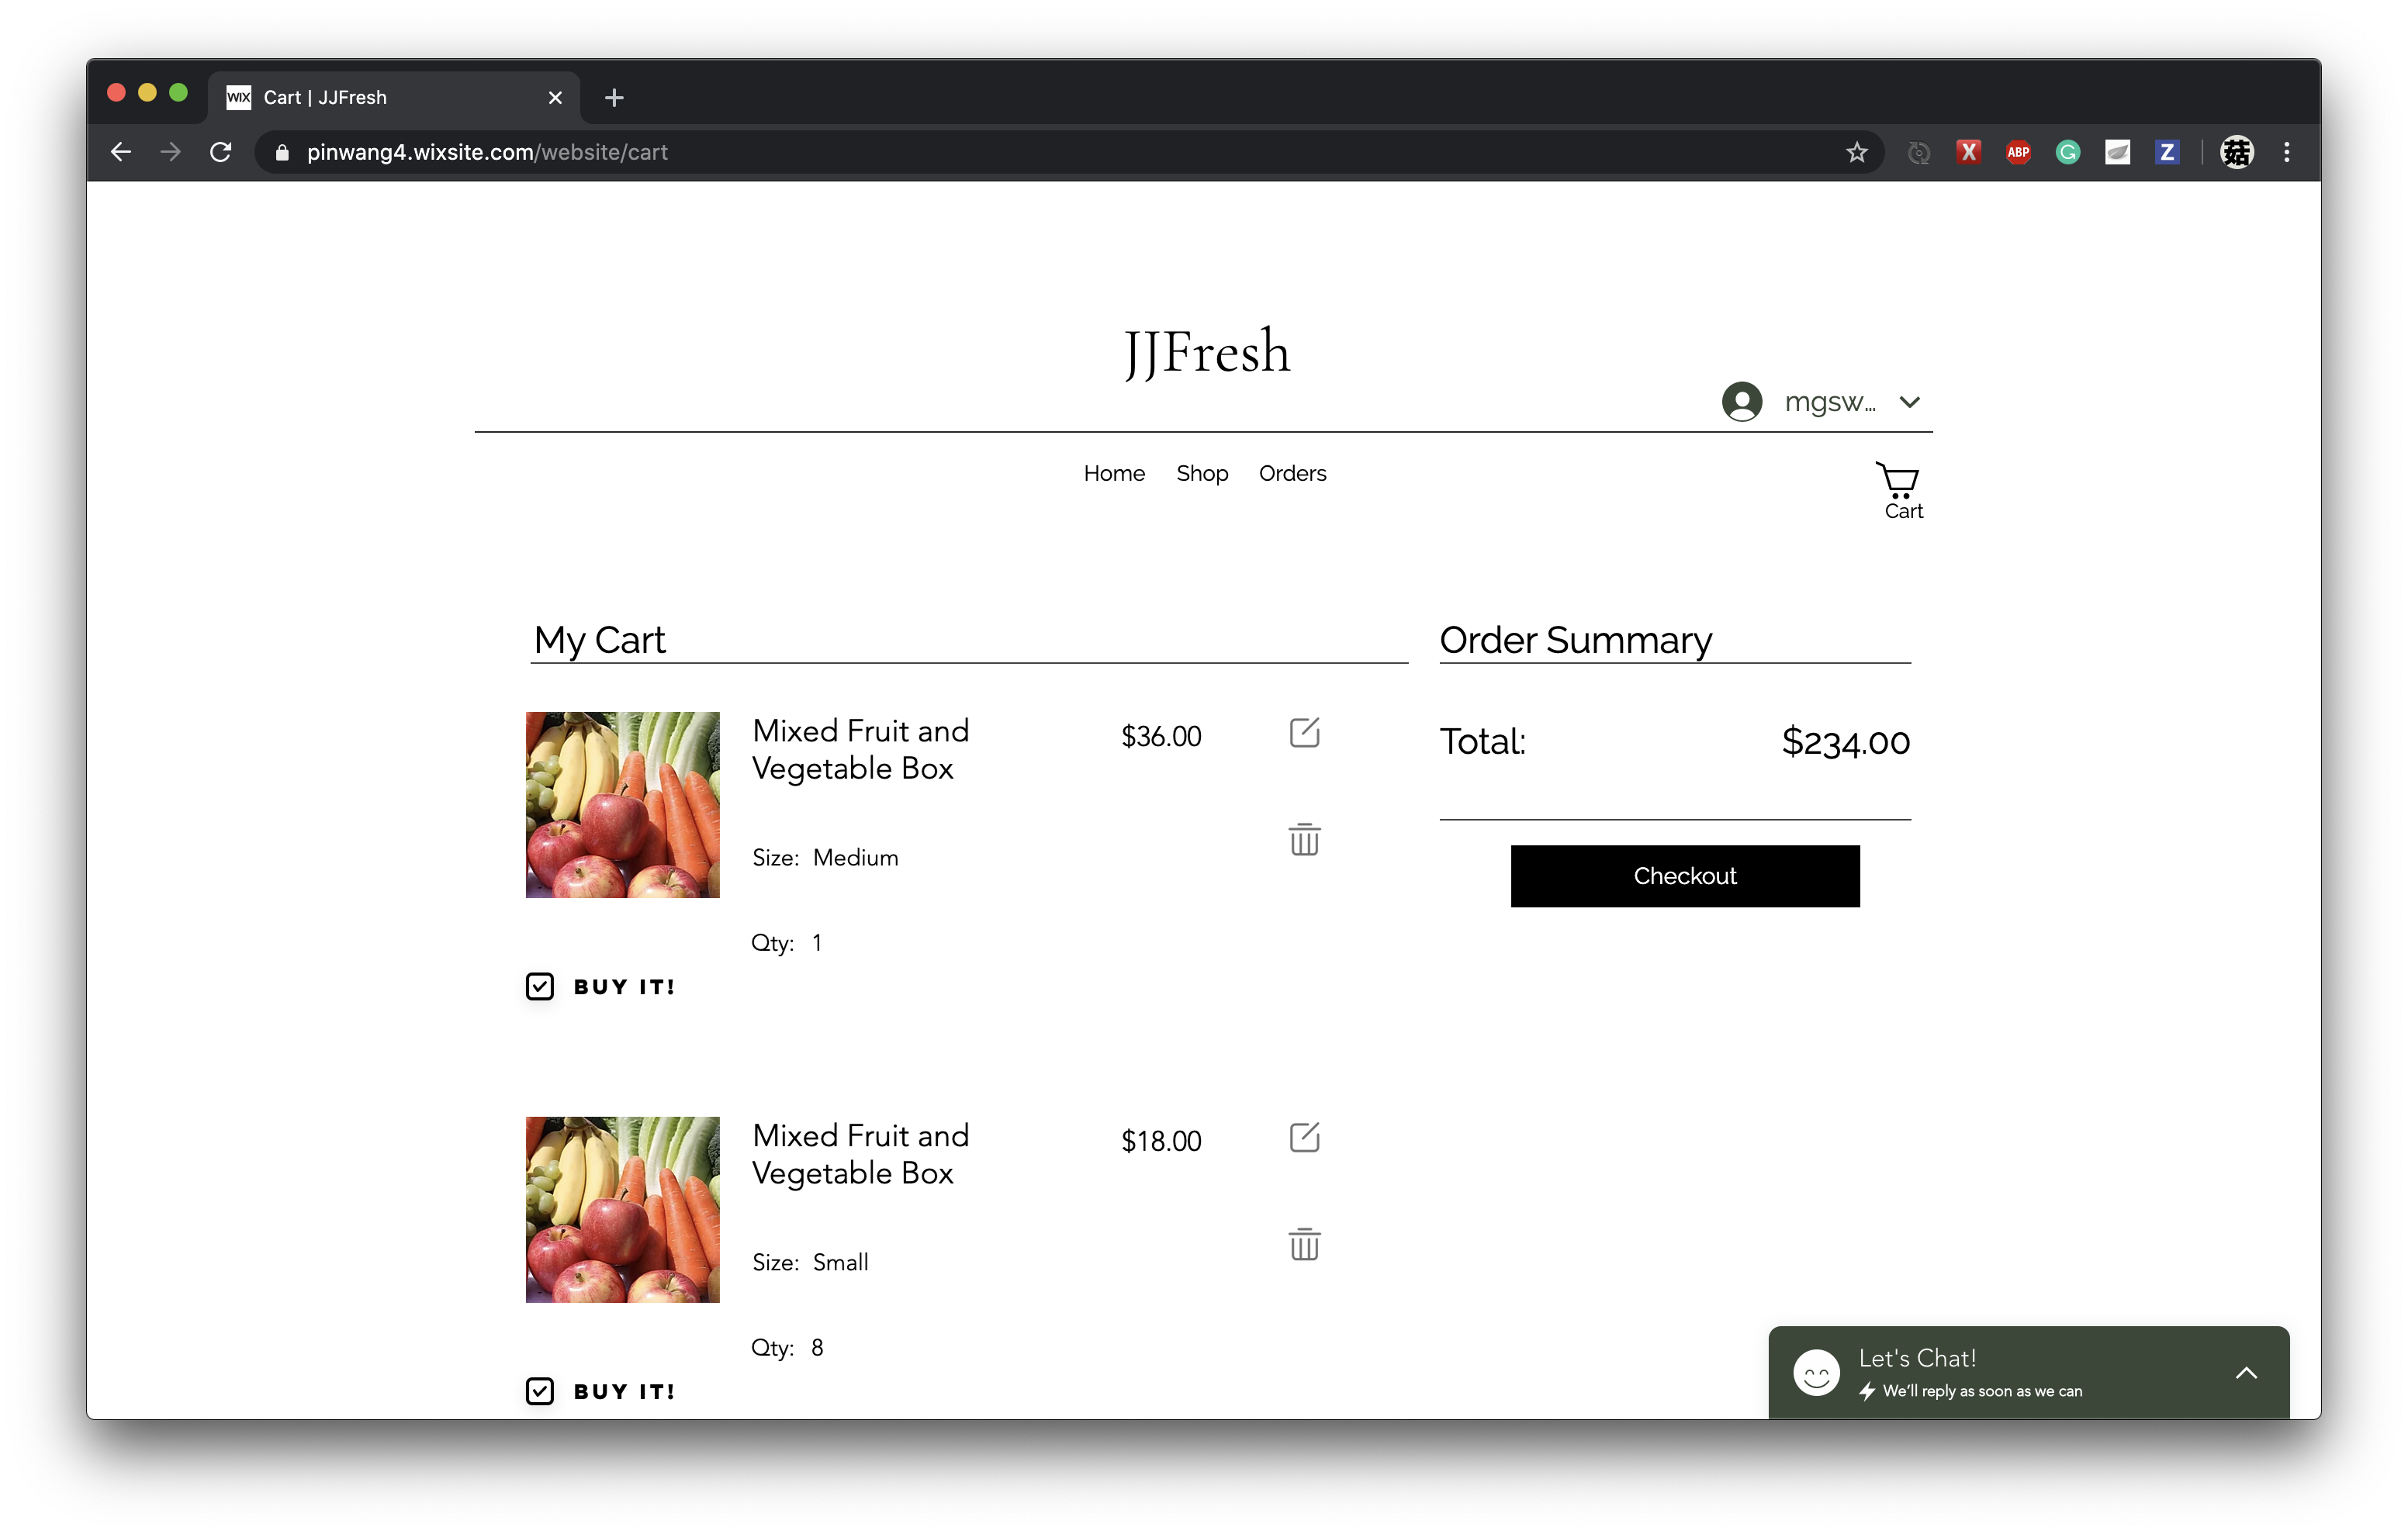
\includegraphics[width=\textwidth]{Figures/checkoutPage.png}
\caption{Screenshot of Checkout page}
\label{fig:checkoutPage}
\end{figure}

\clearpage
\textbf{Delivery Date Selete page}
\begin{figure}[htp]
\centering
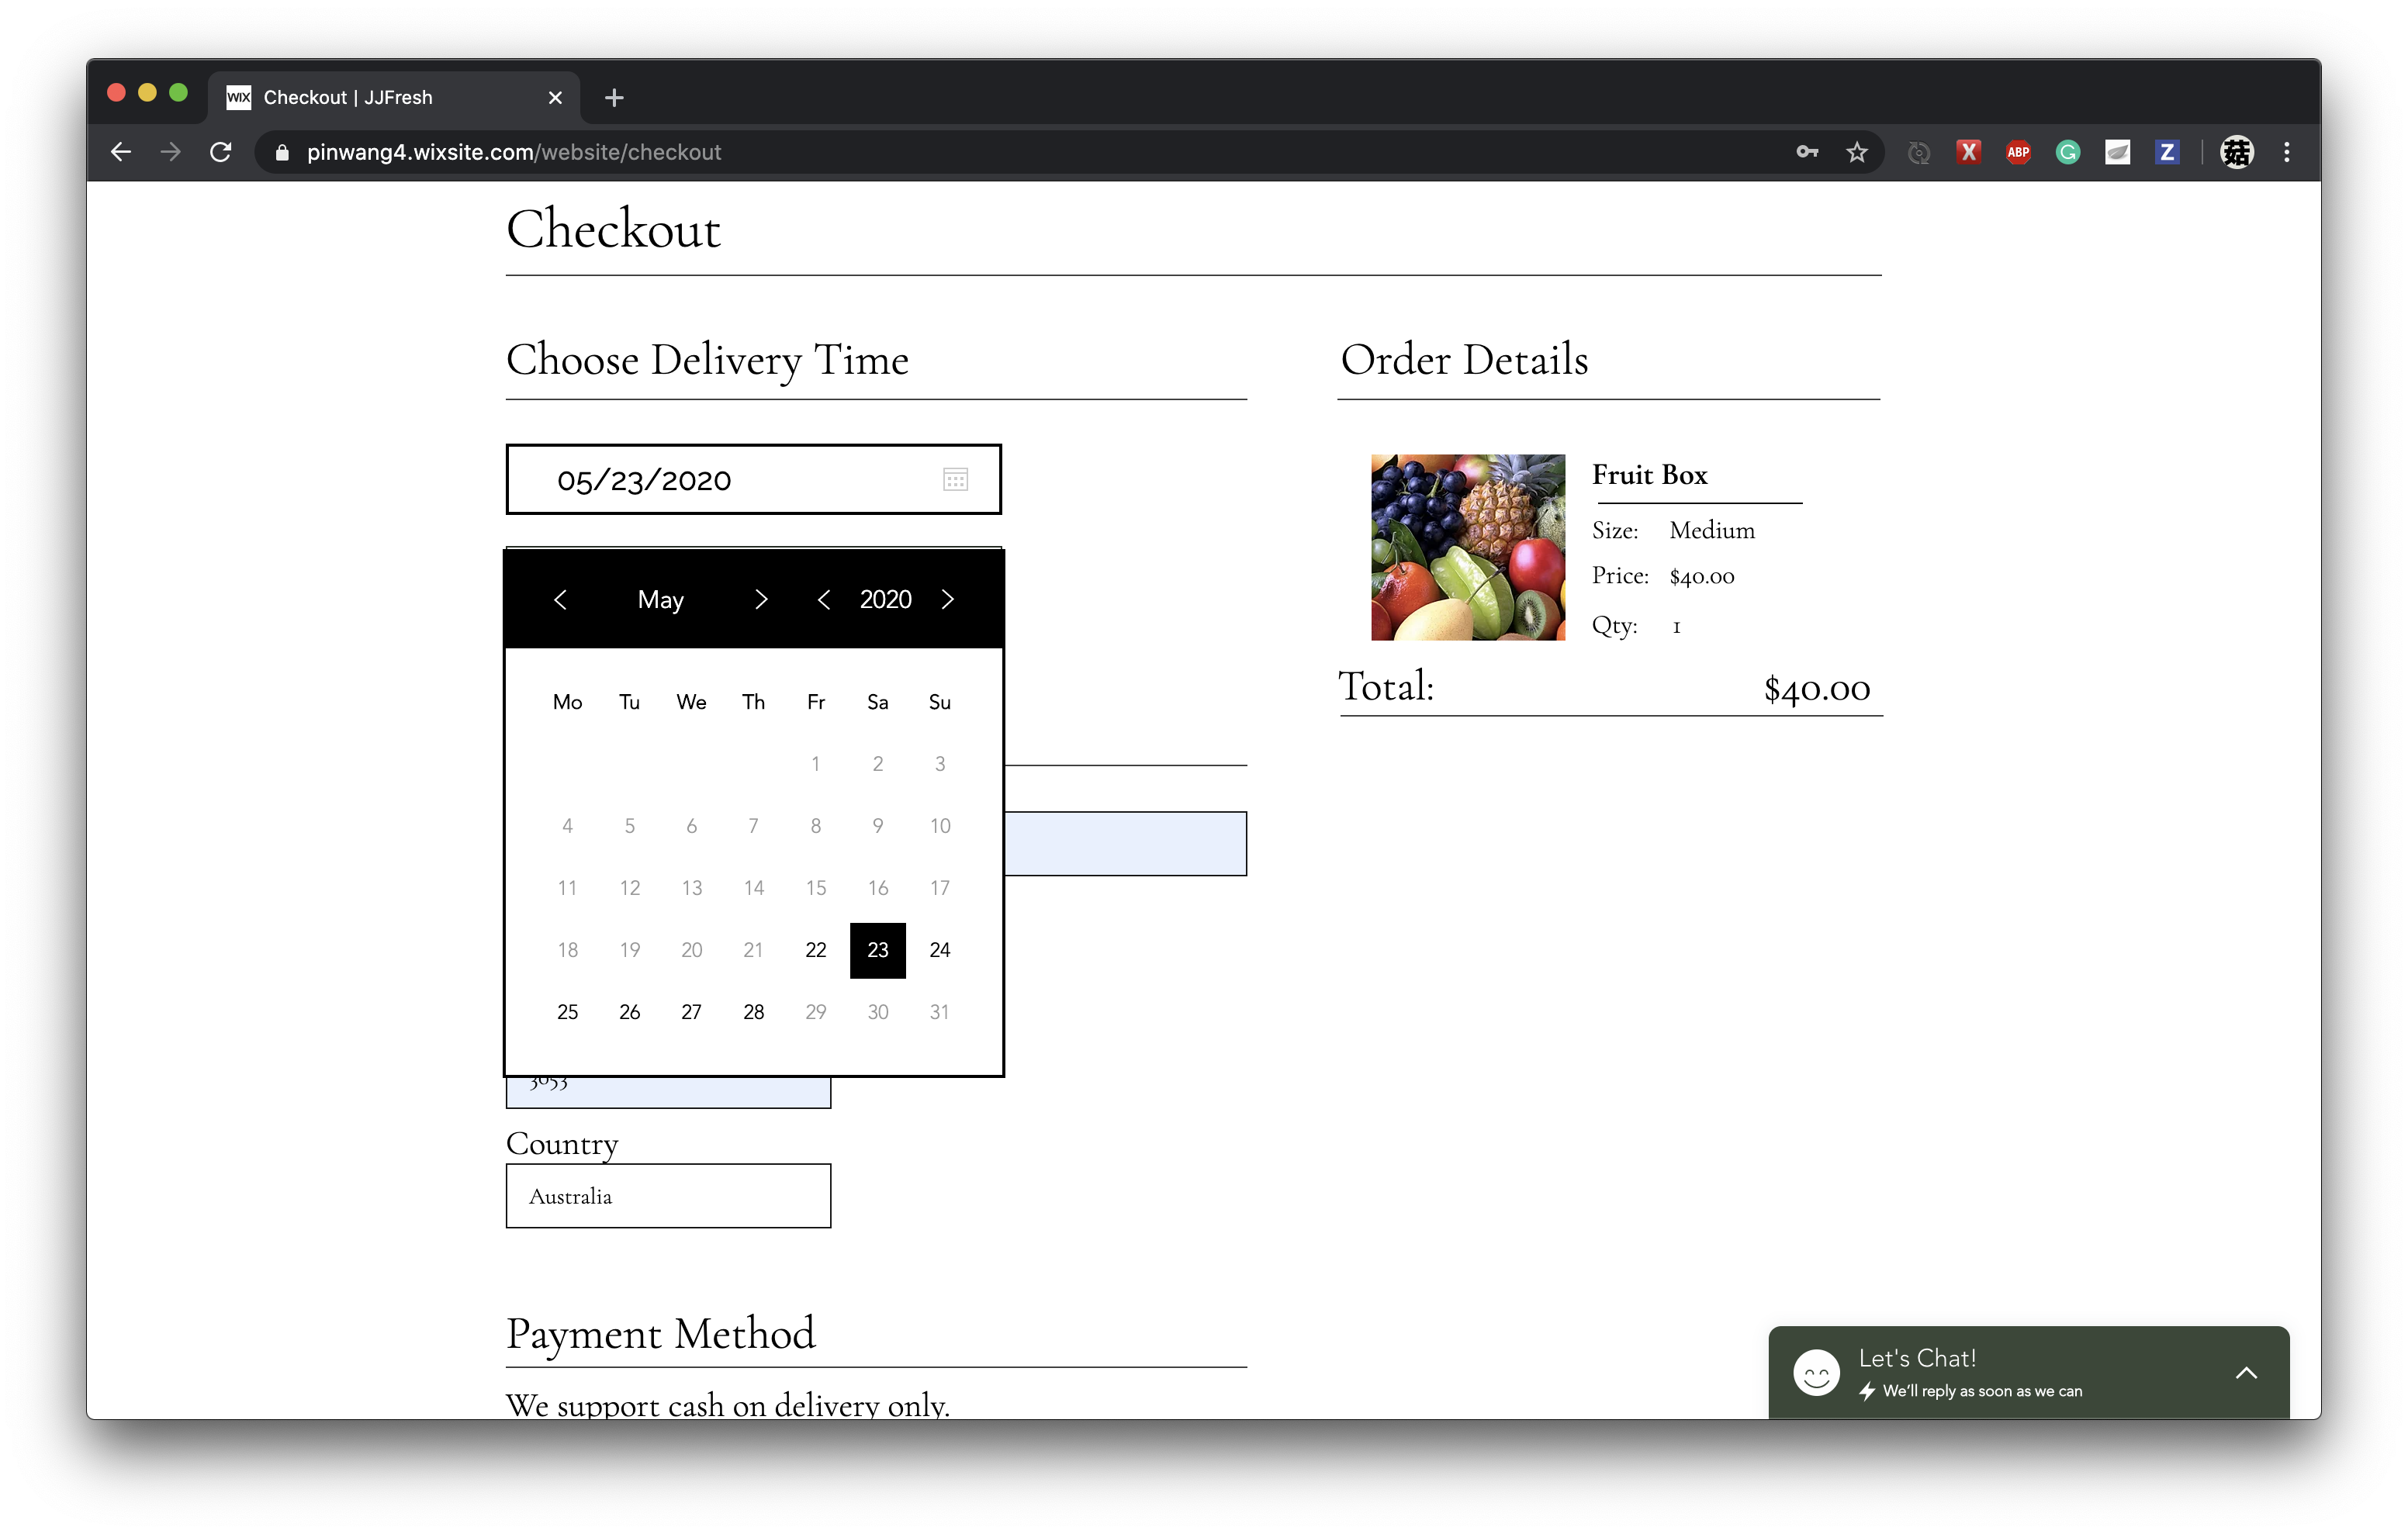
\includegraphics[width=\textwidth]{Figures/dateSelect.png}
\caption{Screenshot of Delivery Date Select}
\label{fig:dateSelect}
\end{figure}

\clearpage
\textbf{Customers can cancel their orders}
\begin{figure}[htp]
\centering
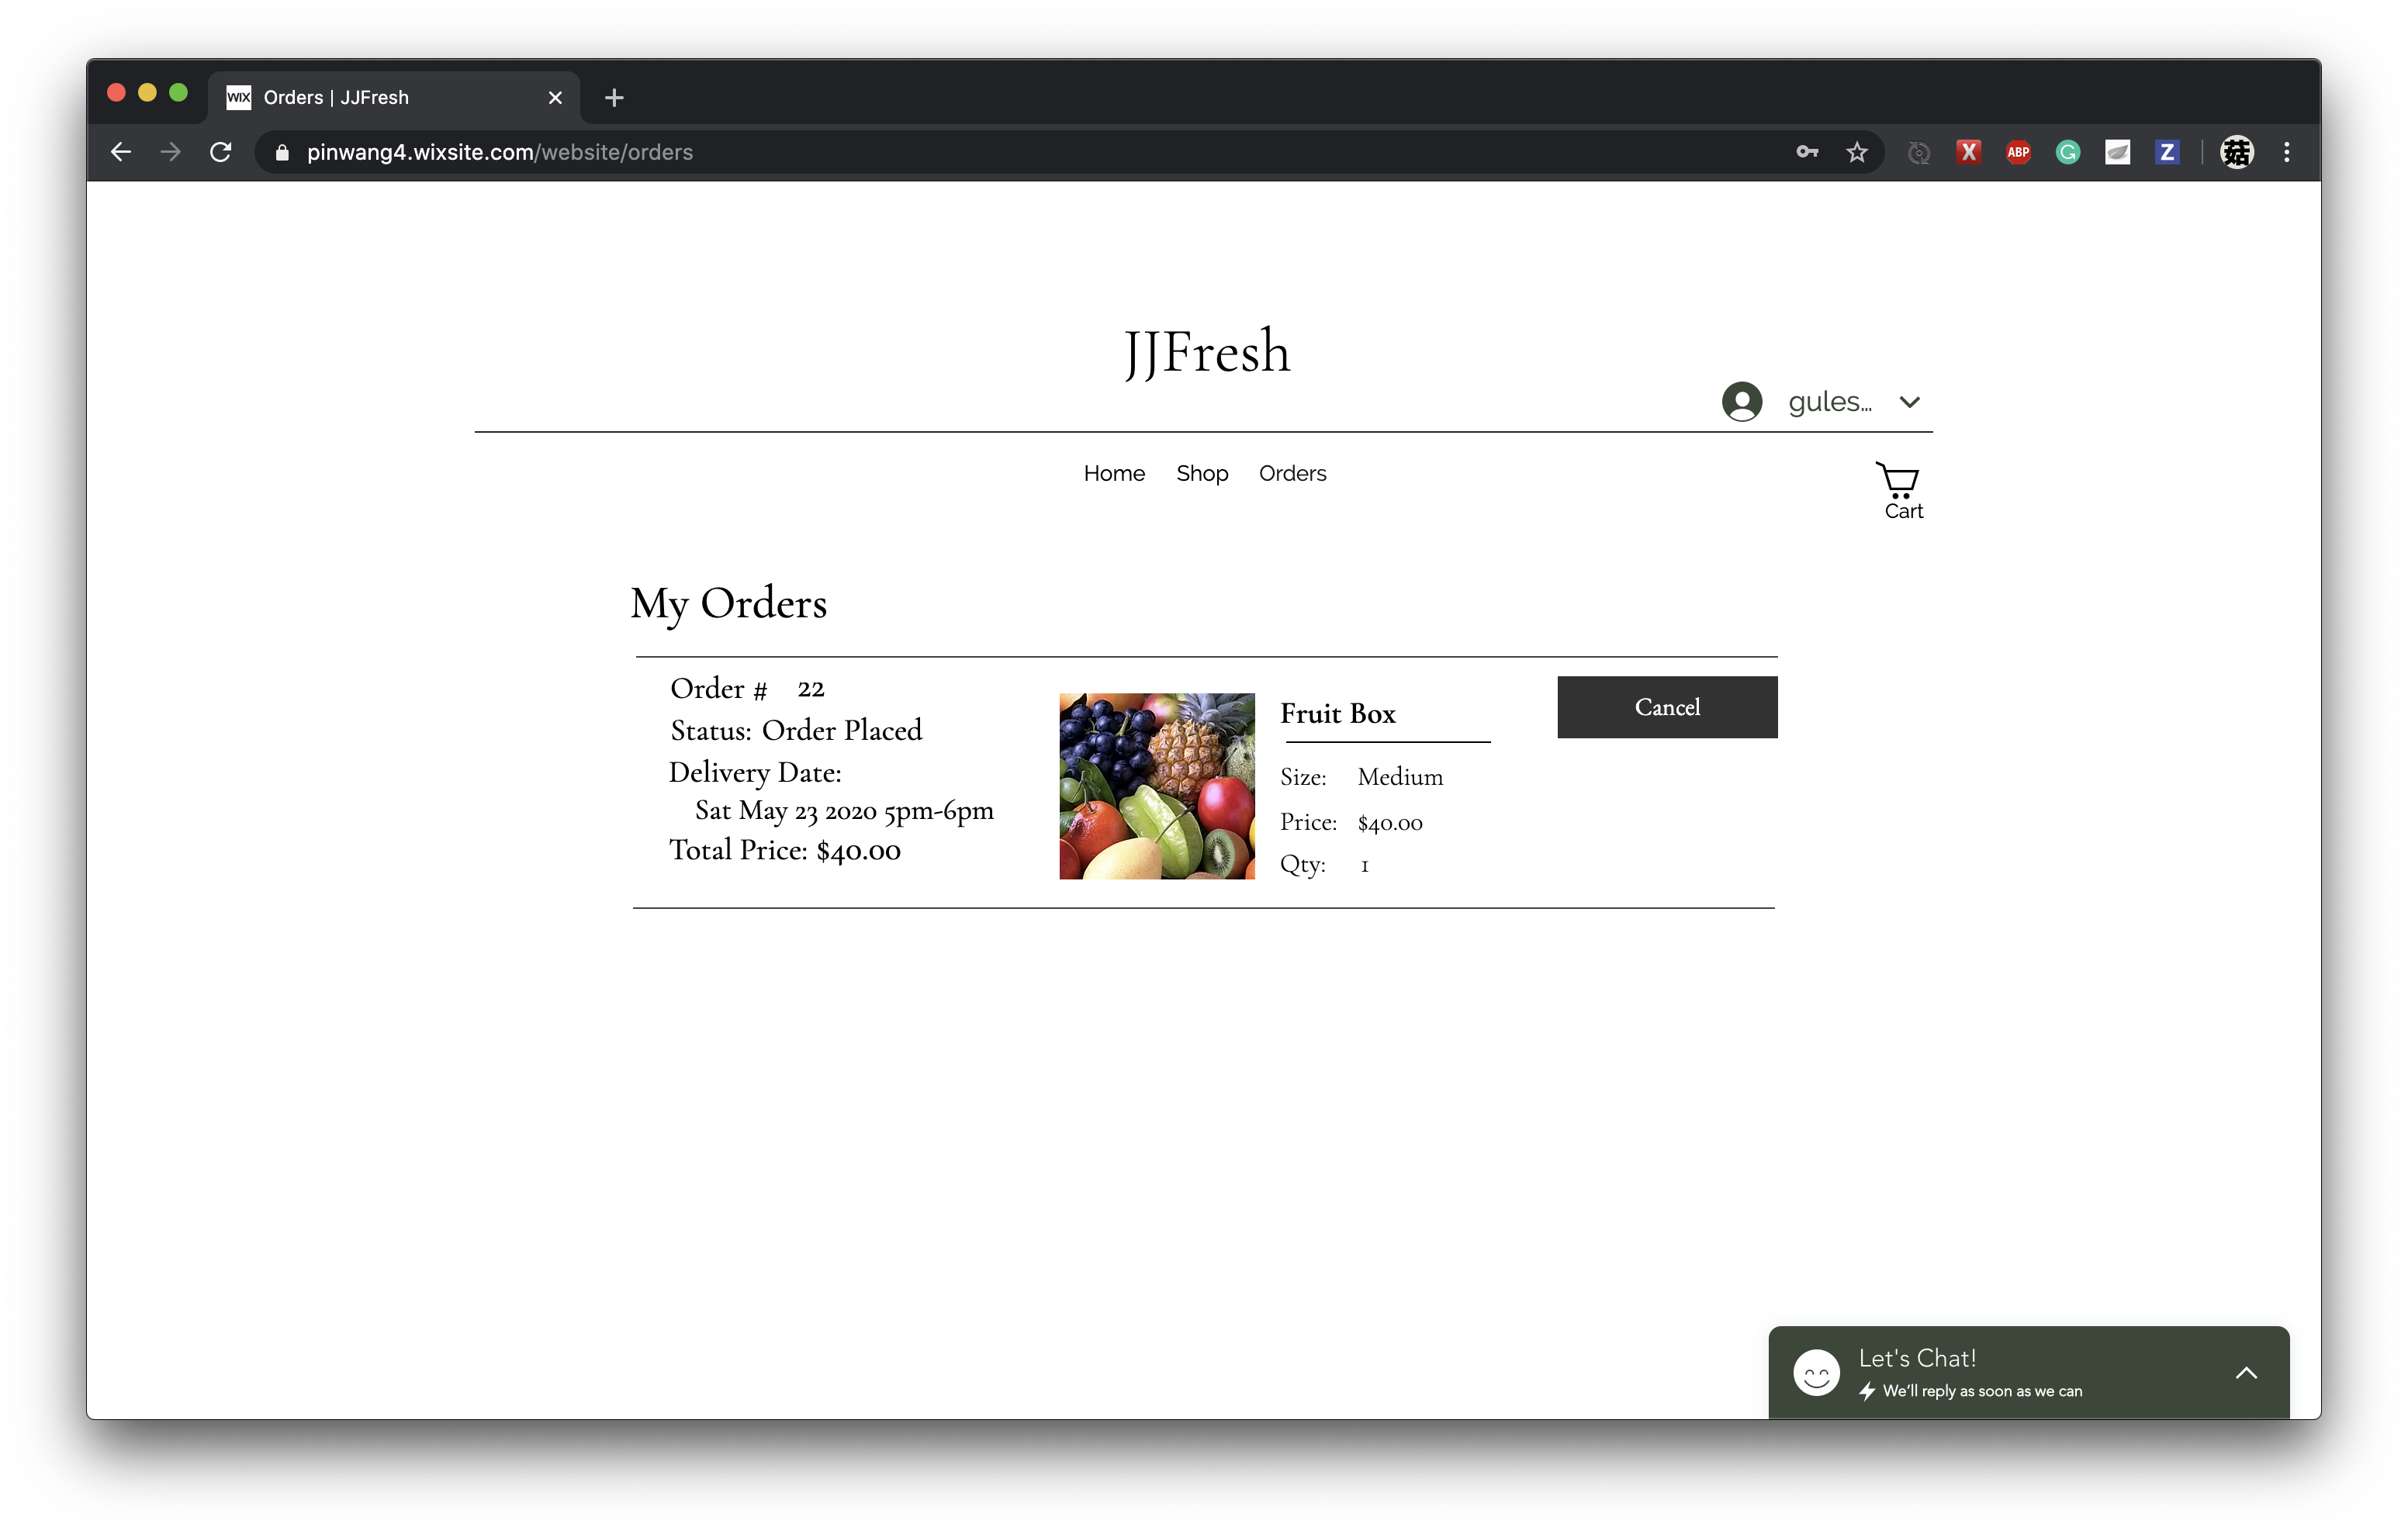
\includegraphics[width=\textwidth]{Figures/customerOrder.png}
\caption{Screenshot of Customers order management page}
\label{fig:customerOrder}
\end{figure}

\clearpage
\textbf{Confirmed email}
\begin{figure}[htp]
\centering
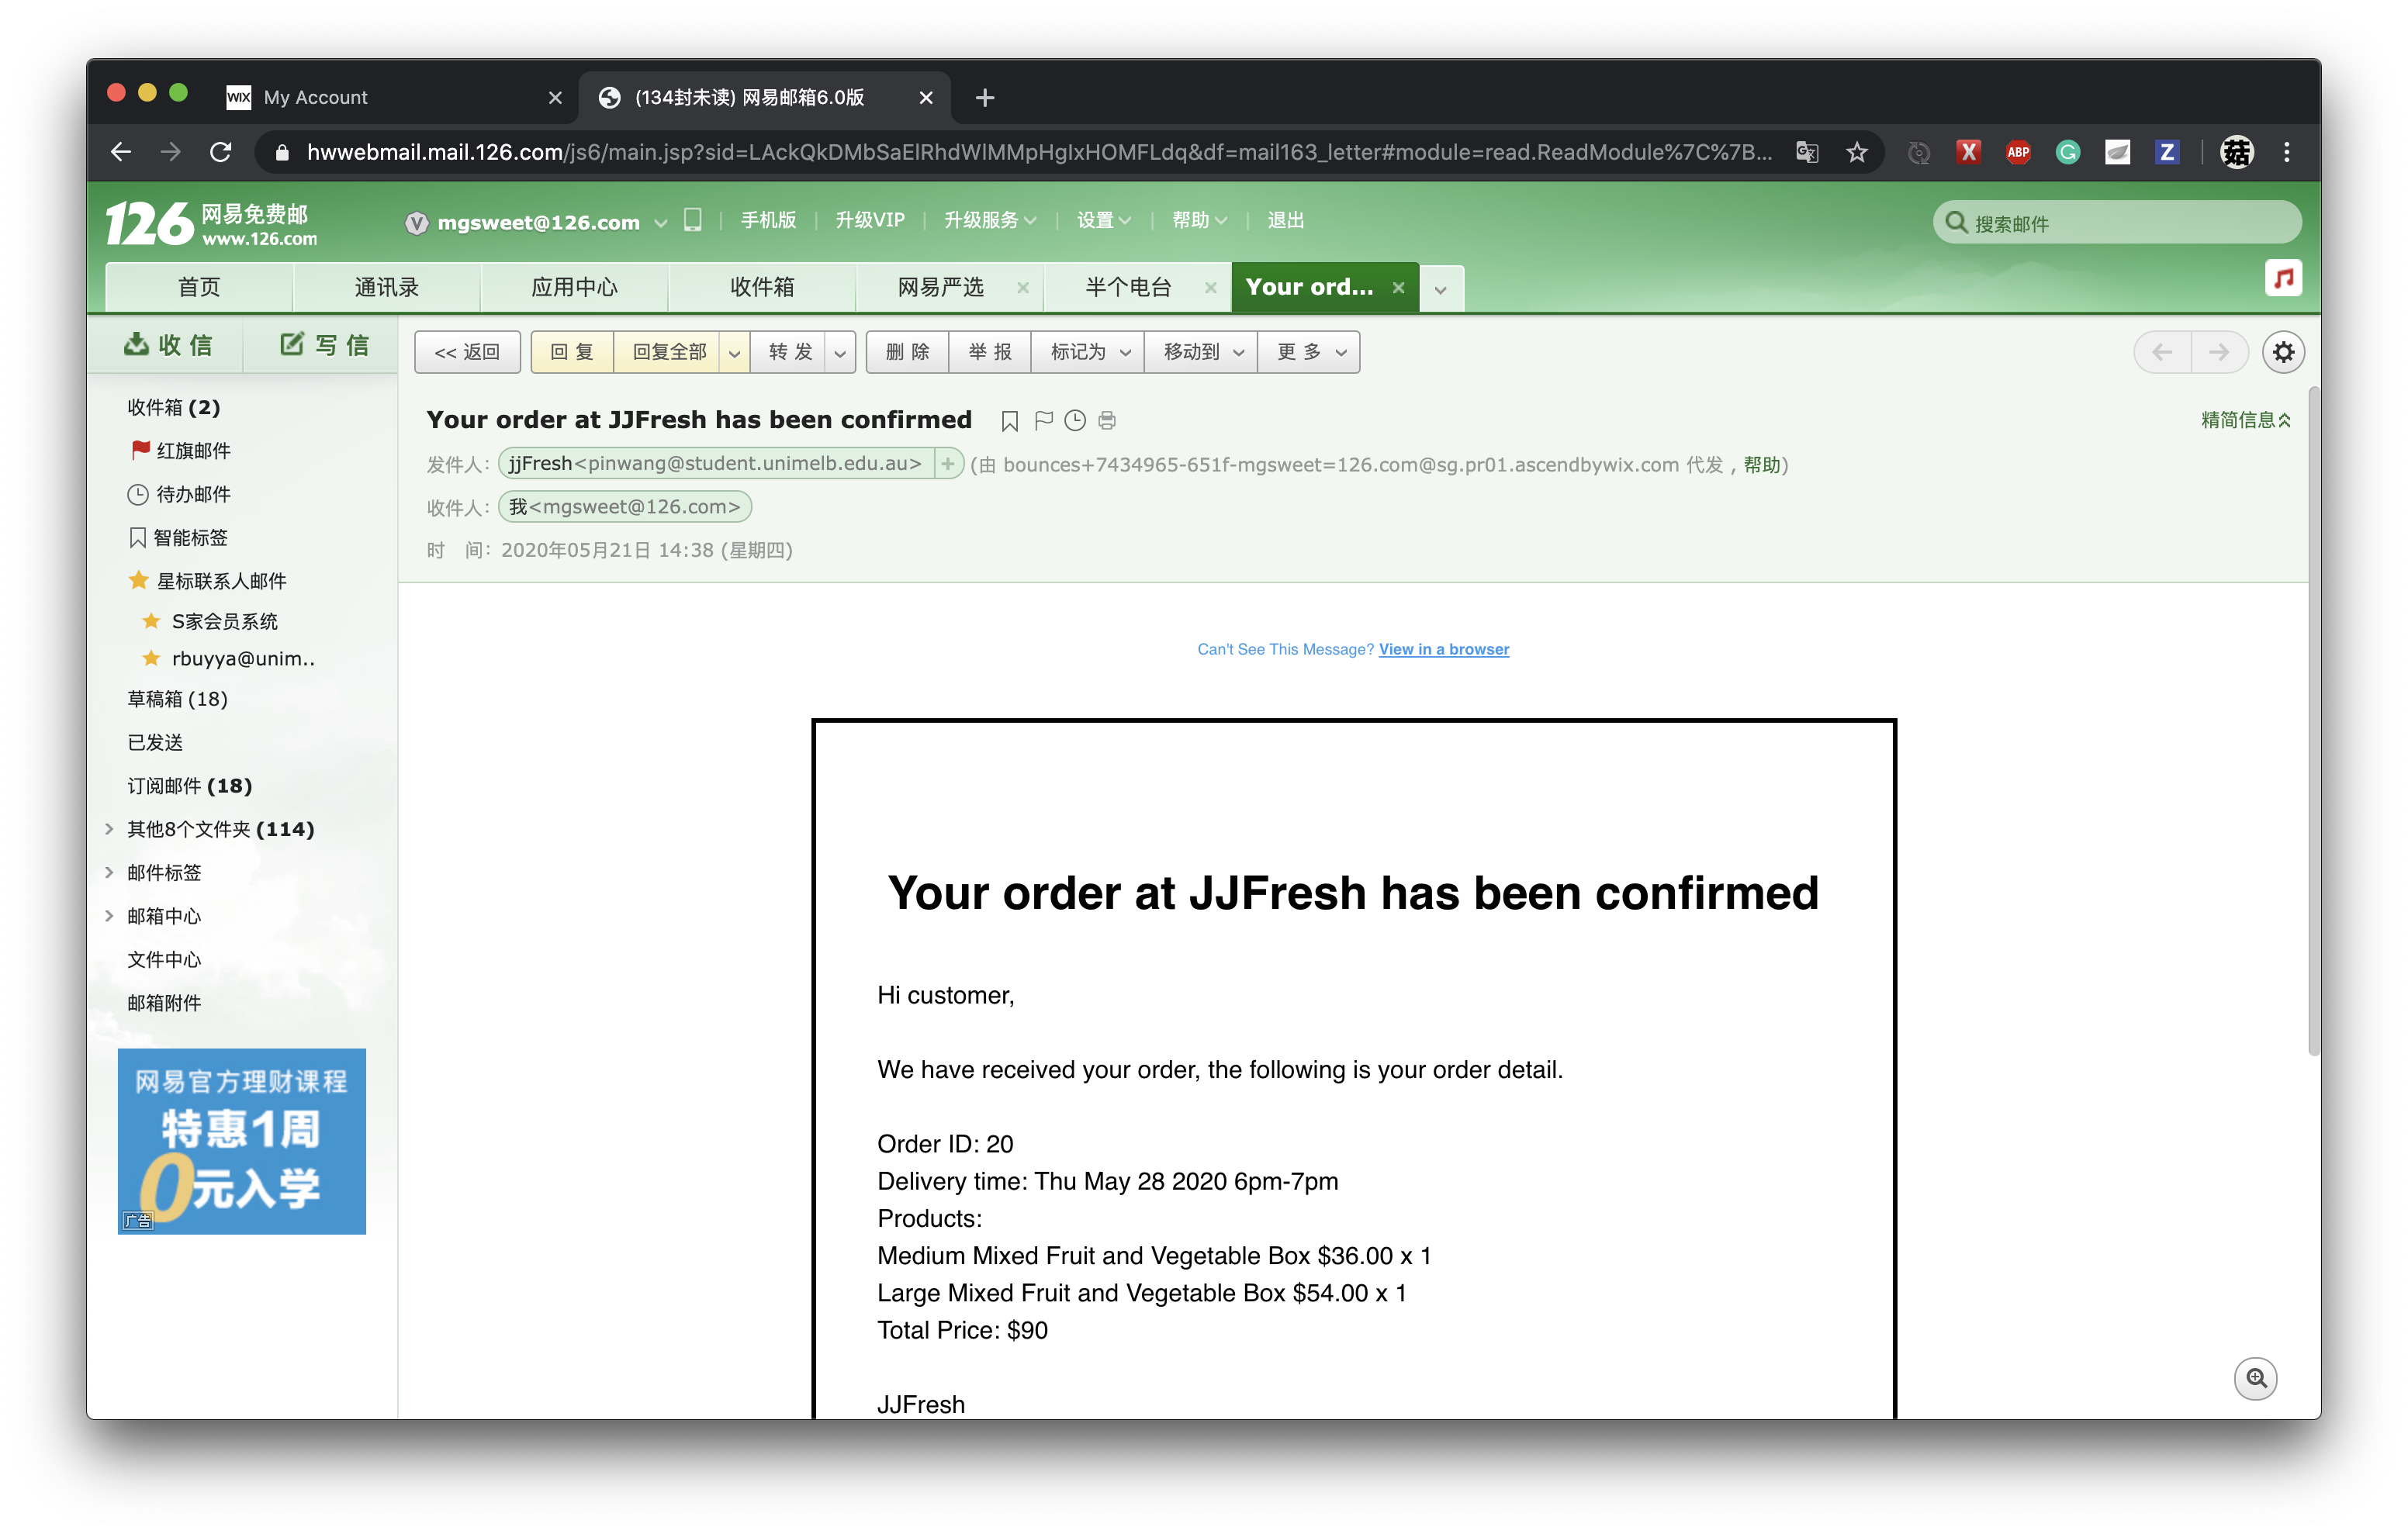
\includegraphics[width=\textwidth]{Figures/confirmedEmail.png}
\caption{Screenshot of confirmed email}
\label{fig:confirmedEmail}
\end{figure}

\clearpage
\textbf{Admin can manage the products}
\begin{figure}[htp]
\centering
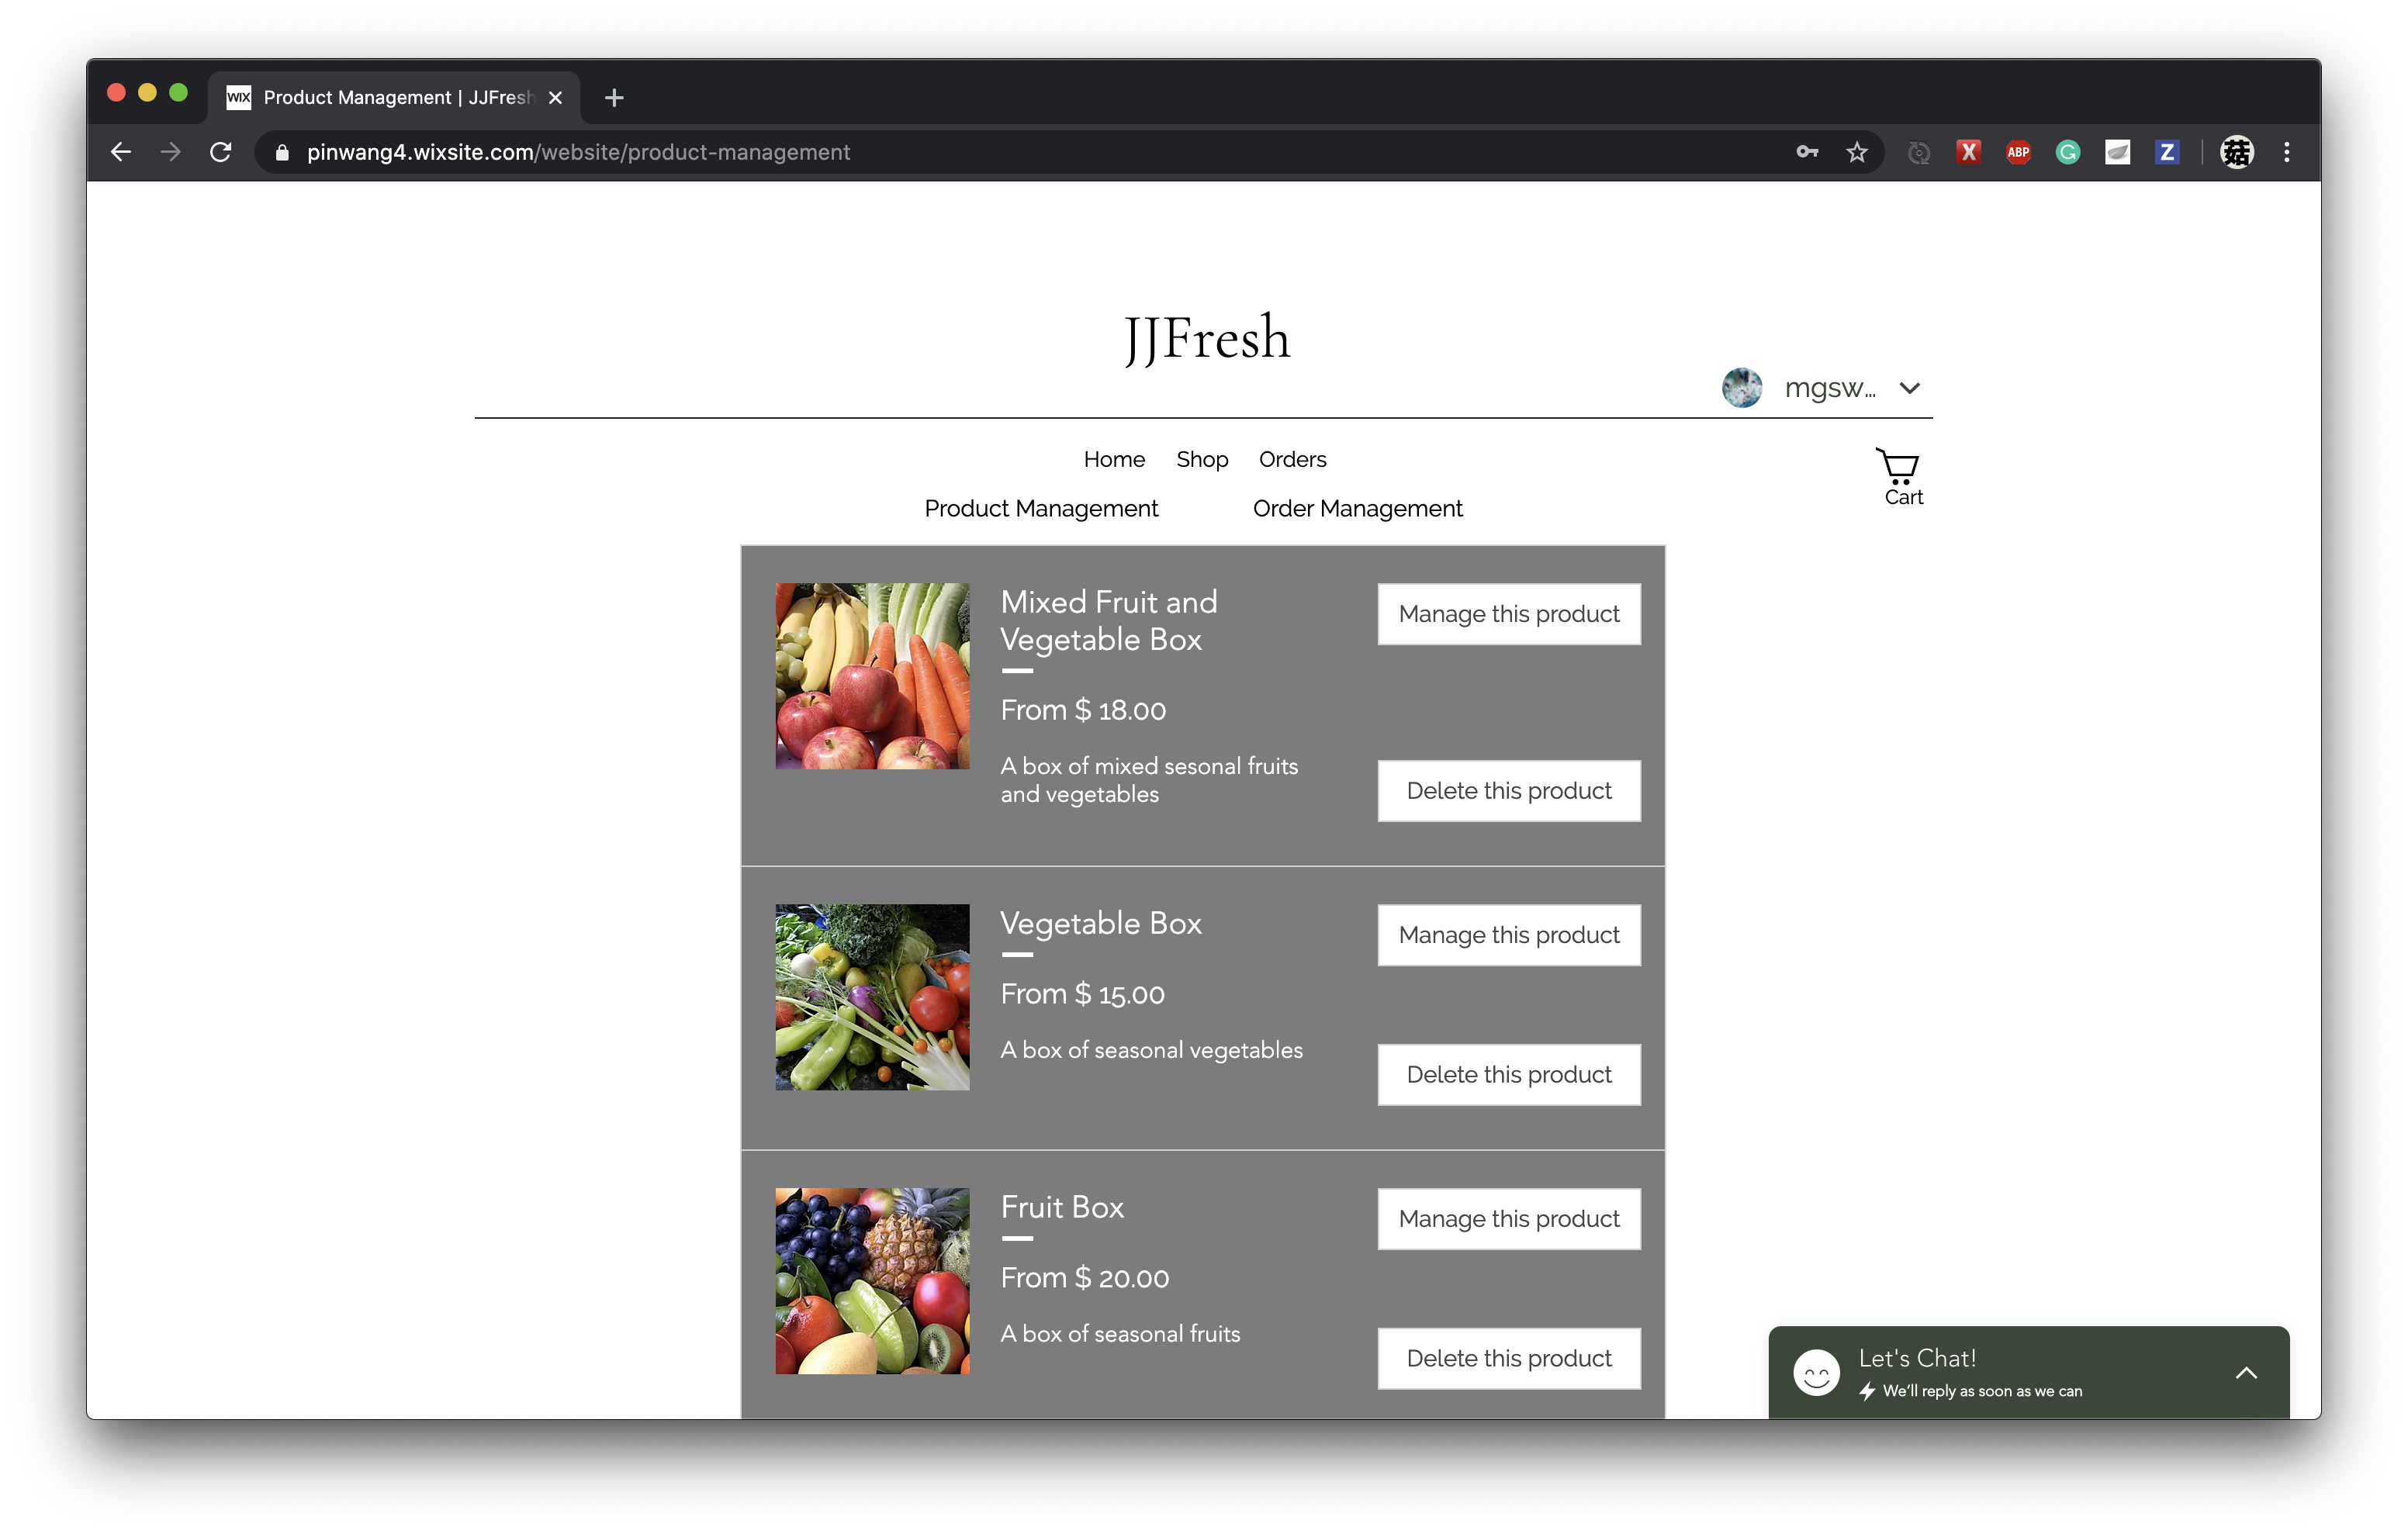
\includegraphics[width=\textwidth]{Figures/adminProduct.png}
\caption{Screenshot of product management}
\label{fig:adminProduct}
\end{figure}

\clearpage
\textbf{Admin can manage the orders}
\begin{figure}[htp]
\centering
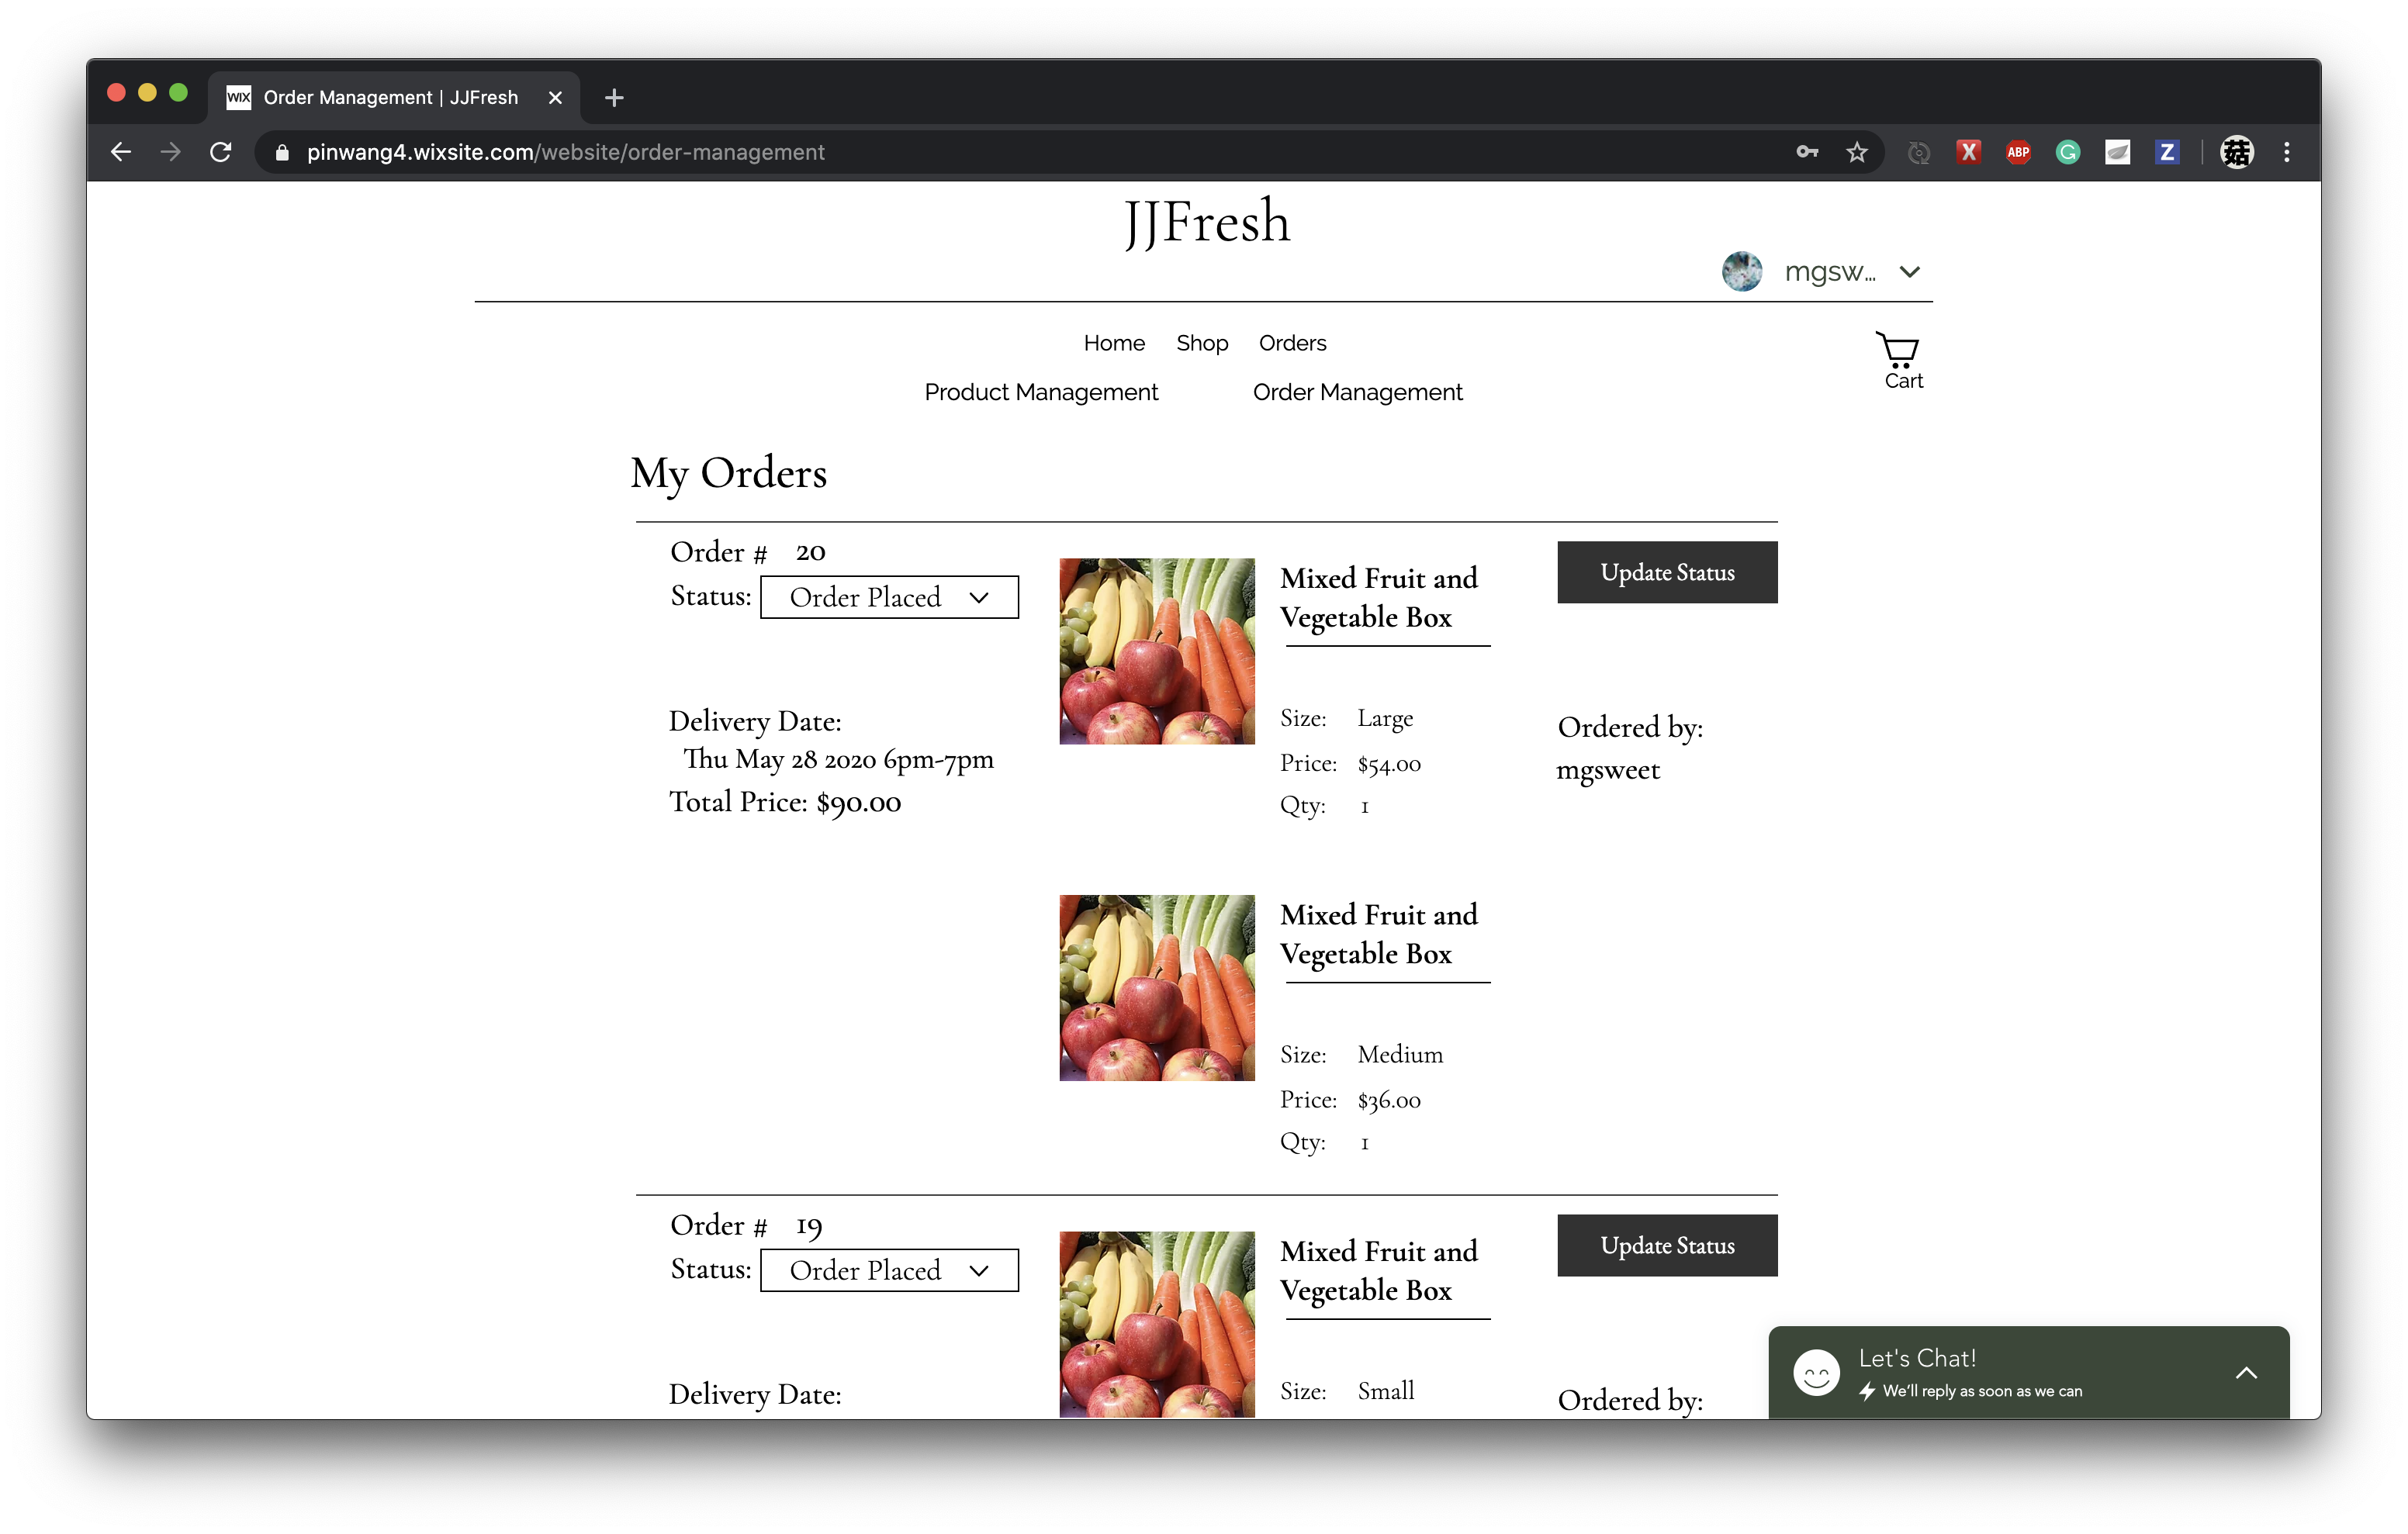
\includegraphics[width=\textwidth]{Figures/adminOrder.png}
\caption{Screenshot of order management}
\label{fig:adminOrder}
\end{figure}

\end{document}